\documentclass[11pt,a4paper]{article}
\usepackage{fontspec,amsmath,amssymb,mathtools}
\providecommand{\mathscr}[1]{\mathcal{#1}}
\DeclareFontFamily{U}{euf}{}
\DeclareFontShape{U}{euf}{m}{n}{<-> eufm10}{}
\usepackage[margin=22mm,headheight=14pt]{geometry}
\usepackage{graphicx,booktabs,longtable,array,calc,enumitem}
\usepackage{needspace,xurl,newunicodechar}
\usepackage[unicode,hidelinks]{hyperref}
\usepackage{bookmark,fancyhdr}
\defaultfontfeatures{Ligatures=TeX}
\usepackage{xeCJK}
\setmainfont{Times New Roman}
\setsansfont{Arial}
\setCJKmainfont[Path=../fonts/,
  BoldFont=NotoSansSC-SemiBold.ttf,
  ItalicFont=NotoSerifSC-Regular.ttf]{NotoSerifSC-Regular.ttf}
\setCJKsansfont[Path=../fonts/,
  BoldFont=NotoSansSC-SemiBold.ttf]{NotoSansSC-SemiBold.ttf}
\setCJKmonofont[Path=../fonts/]{NotoSansSC-SemiBold.ttf}
\xeCJKsetup{PunctStyle=quanjiao,CJKmath=true}
\renewcommand{\figurename}{图}
\XeTeXlinebreaklocale "zh"
\XeTeXlinebreakskip=0pt plus 1pt
\setmonofont{Consolas}[Scale=0.82]
\newfontfamily\extendedlatin{lmroman10-regular.otf}
\newunicodechar{ő}{{\extendedlatin\char"0151}}
\newunicodechar{ű}{{\extendedlatin\char"0171}}
\setlength{\emergencystretch}{4em}
\setlength{\parindent}{1.5em}
\setlength{\parskip}{2.5pt plus 1pt}
\linespread{1.10}
\allowdisplaybreaks[3]
\raggedbottom
\clubpenalty=10000
\widowpenalty=10000
\displaywidowpenalty=10000
\setcounter{secnumdepth}{-1}
\providecommand{\tightlist}{\setlength{\itemsep}{0pt}\setlength{\parskip}{0pt}}
\newcommand{\passthrough}[1]{#1}
\setlist{itemsep=2pt,parsep=0pt}
\makeatletter
\renewcommand\section{\@startsection{section}{1}{\z@}{-2.8ex plus -1ex minus -.2ex}{1.1ex plus .2ex}{\normalfont\large\bfseries}}
\renewcommand\subsection{\@startsection{subsection}{2}{\z@}{-2.1ex plus -.8ex minus -.2ex}{.8ex plus .2ex}{\normalfont\normalsize\bfseries}}
\renewcommand\subsubsection{\@startsection{subsubsection}{3}{\z@}{-1.8ex plus -.5ex minus -.2ex}{.6ex plus .2ex}{\normalfont\normalsize\bfseries}}
\makeatother
\pagestyle{fancy}
\fancyhf{}
\fancyhead[C]{\small 竞赛图中的 Hamilton 计数}
\fancyfoot[C]{\small\thepage}
\renewcommand{\headrulewidth}{0pt}
\hypersetup{pdftitle={竞赛图路径计数的永久式估计（技术补充）},pdfauthor={刘星辰、叶祥宇}}
\begin{document}
\thispagestyle{plain}
\begin{center}
{\Large\bfseries 竞赛图路径计数的永久式估计（技术补充）\par}
\vspace{9pt}
{\normalsize 刘星辰、叶祥宇\par}
\vspace{5pt}
{\small 2026 年 10 月 28 日\par}
\end{center}
\vspace{3pt}
\begin{quote}
\noindent\textbf{摘要.} Divoux--Wang 已证明 \(n\) 阶竞赛图的最大 Hamilton 路径数为 \((L+o(1))n!/2^{n-1}\)，其中 \(L=\cosh1/\cos1\)。本文是配套合稿的技术补充，详述永久式近似、不同的行列删集下的对角缩放，以及路径计数恒等式中的加权求和。这些估计用于合稿对全体竞赛图的 \(O(n^{-1})\) 归一化误差证明。作为应用，本文保留下界 \((L-O(n^{-1}))n!/2^{n-1}\) 与上界 \((C_*+O(n^{-1}))n!/2^{n-1}\) 的推导，其中 \(C_*=(3\pi^4+4\pi^2-32)/(\pi^4+4\pi^2-32)>L\)。此常数因子上界已由 Divoux--Wang 的首项结果涵盖；保留它是为了说明，仅用谱半径和平方频率之和即可完成计数估计的最后一步。
\end{quote}
\Needspace{5\baselineskip}
\section{1. 引言}\label{ux5f15ux8a00}

竞赛图是完全图的一个定向。记 \(H(T)\) 为竞赛图 \(T\) 的有向 Hamilton 路径数，按顶点顺序计数，并令 \(P(n)=\max_{|V(T)|=n}H(T)\)、\(\mu_n=n!/2^{n-1}\)；圈数的随机期望记为 \(\nu_n=(n-1)!/2^n\)（\(n\ge3\)）。

Szele {[}10{]} 用期望的线性性给出了这个问题的第一个下界。在均匀随机竞赛图中，一个给定的顶点排列以概率 \(2^{-(n-1)}\) 形成有向路径，故路径数的期望为 \(\mu_n\)，从而 \(P(n)\ge\mu_n\)。对 \(n\ge3\)，同样的计算给出圈数期望 \(\nu_n\)。Szele 还证明了上界 \(P(n)=O(n!2^{-3n/4})\)，并猜想 \((P(n)/n!)^{1/n}\) 趋于 \(1/2\)。因此，最初的问题是确定路径数的指数增长率。

Alon {[}2{]} 通过永久式解决了这一问题。邻接矩阵 \(A\) 的永久式等于覆盖全部顶点的互不相交有向圈族的数目，因而是 Hamilton 圈数的上界。将 Brégman 不等式用于 \(\operatorname{per}A\)，再利用出度之和为 \(\binom n2\)，可以证明所得上界在出度尽可能均匀时最大。由圈数上界加上一个新顶点的构造，Alon 得到 \(P(n)=O(n^{3/2}\mu_n)\)。Friedgut--Kahn {[}7{]} 以熵方法细化了这一类计数，将圈数上界改进为 \(O(n^\alpha\nu_n)\)，其中 \(\alpha\approx1.249\)；相应的路径上界具有同样的多项式因子。这些结果确定了指数增长率，但上、下界之间仍相差一个随 \(n\) 增长的多项式。

提高下界则需要改变边的随机定向方式。Adler、Alon 和 Ross {[}9{]} 在完全图中选取近乎覆盖全部边的边不交三角形族，再将各三角形独立、均匀地定向为有向三圈。若一个顶点排列中有某个三角形连续出现，该排列形成有向路径的概率便比独立定向模型更大。对均匀随机的顶点排列，他们用 Brun 筛证明这类连续出现的次数趋于均值为一的 Poisson 分布，由此得到下界 \((e-o(1))\mu_n\)；同一构造也改进了圈数下界。Wormald {[}6{]} 进一步考虑固定基图的随机吹胀：块间方向由基图决定，块内分别取均匀随机竞赛图或随机正则竞赛图。沿一个无穷阶数序列，圆环基图给出的圈数下界常数超过 \(2.85588\)，其数值计算又预示了约为 \(2.855958\) 的极限常数。不过，这些构造只给出下界，尚不能排除其他竞赛图具有更多的 Hamilton 圈或路径。

Divoux--Wang {[}12{]} 确定了这个常数，证明全体竞赛图的最大圈数为 \((L+o(1))\nu_n\)，最大路径数为 \((L+o(1))\mu_n\)，其中 \(L=\cosh1/\cos1\)。他们仍从永久式出发，但保留了仅由度数给出的上界无法反映的矩阵信息。对于圈数至少达到随机期望的竞赛图，Brégman 不等式先限制其度差平方和；删去少量度差过大的顶点后，剩余邻接矩阵经标量归一化后接近双随机矩阵。为计入被删顶点，他们按 Hamilton 圈在这些顶点上形成的有向路段分类，将每类路段及其连接端点编码为核心上的加权矩阵。随后利用 Sinkhorn 缩放、McCullagh 型永久式近似以及 Liu 的行列式---永久式恒等式，将圈数归结为反对称矩阵的行列式比值。Fang--Huang {[}11{]} 的矩阵比较定理给出该比值的上界，圆环图及其偶阶删点图达到相同的渐近值。路径结论再由增添顶点的论证得到。

既然最优首项常数已经确定，进一步的问题在于控制有限阶误差。本文为配套合稿详述这部分估计：永久式近似须对矩阵类一致，非主子矩阵的缩放误差须保留对行列删集大小的依赖，最后还须在路径计数恒等式中对所有删集求和。第 7 节将这些估计用于全体竞赛图，第 8 节则对圆环图及其偶阶删点图给出双侧近似。合稿在此基础上调用 Fang--Huang {[}11{]} 的矩阵比较，得到归一化误差为 \(O(n^{-1})\) 的路径计数结论。

为使上述估计的用途在本文内完整呈现，我们在最后一步仅用谱半径界与平方频率之和，得到下列辅助估计。其中 \(C_*>L\)，故其上界在充分大阶数时已由 Divoux--Wang 的 \((L+o(1))\mu_n\) 结果推出。这里保留直接证明，是因为它完整展示了从永久式近似、删除和缩放到路径求和的过程；这些计算也是合稿中更精确上界所用的估计。

\Needspace{7\baselineskip}
\textbf{命题 1.1（辅助估计）。} 存在绝对常数 \(K,n_0\)，使所有 \(n\ge n_0\) 满足

\[(L-K/n)\mu_n\le P(n)\le(C_*+K/n)\mu_n,
\qquad
C_* =\frac{3\pi^4+4\pi^2-32}{\pi^4+4\pi^2-32}.\]

\Needspace{5\baselineskip}
\subsection{1.1 永久式估计与路径计数}\label{ux6c38ux4e45ux5f0fux4f30ux8ba1ux4e0eux8defux5f84ux8ba1ux6570}

McCullagh {[}5{]} 已在适度偏离条件下给出永久式的行列式近似，相对误差为 \(O(n^{-1})\)。Divoux--Wang {[}12{]} 为其计数问题证明了对矩阵类一致的 \(1+o(1)\) 版本；对于本文计数所用的非负矩阵，保留其证明中的定量误差，也可提取 \(O(n^{-1})\) 的误差阶。第 3 节给出这一近似在固定元素界和固定奇异值谱隙下的详细证明，并明确误差常数的依赖。矩阵随竞赛图而变，在同一个图中又随删集而变，误差常数须同时适用于这些矩阵，才能把永久式近似代入计数恒等式后求和。

证明从永久式的系数展开出发，对行指标和列指标的互异性分别作容斥。双中心化使含一度顶点的项消失；二度分量的总和由高斯配对计算，得到行列式主项。其余分量先收缩二度链，再按边数与顶点数之差估计。这样可以控制随矩阵阶数增长的一段系数。尾项另作估计：先用永久式极化化为半正定情形，再用 Han--Niles-Weed {[}3, 引理 4.3--4.4{]} 所用的复高斯矩与 AM--GM 估计控制其模，最后应用 Cauchy 系数估计。两部分合起来给出所需误差，不必将形式级数代入未经证明的收敛区域。

路径部分采用 Irving--Omar {[}1{]} 所讨论的行列式---永久式恒等式的竞赛图特例：

\[H(T)=\sum_{U\subseteq V(T)}\det(I+A[U])\operatorname{per}A[U^c].\]

右端各项均非负，因而可以直接估计每个永久式，再对删集求和。大删集的总贡献由阶乘尾界控制；对其余删集，永久式估计还须经过对角缩放，才能用于原来的邻接矩阵。求和时保留删集大小的原权重，并利用其各阶固定矩可求和的性质；若一律用最大的删集大小代入，就会产生额外的对数因子。

少量度差很大的顶点使这一步较为复杂。我们按异常顶点集及其补集将矩阵分为四块，再按跨块匹配展开永久式。一个匹配在剩余部分占用的行、列可能具有不同的指标，因此只估计主子矩阵不够。第 4 节同时处理不同的行删集与列删集，并估计对角缩放因子和高斯行列式因子的变化。这与 Divoux--Wang 对圈在异常集内形成的有向路径段分类有所区别：这里的求和对象是永久式展开中的行列匹配。

为了得到对所有竞赛图成立的路径上界，只需考虑 \(H(T)\ge\mu_n\) 的图。Brégman 不等式先限制出度的离差平方和；该量过大时可直接给出充分小的上界。若仍有异常顶点，则利用上述跨块展开估计。其余图的缩放计算中，度差产生一个负指数因子。中间某些误差为平方根量级，单独取绝对值会丢失所需精度；将它们与负指数合并估计，最终仍只损失 \(O(n^{-1})\)。此时主项为

\[\rho_n(S)=\frac{\det(I+S/n)}{\det(I+iS/n)},\qquad S=A-A^T.\]

谱半径界限制各个平方频率的大小，Frobenius 范数又确定其总和。将这两个条件用于谱比值的乘积表达式，得到辅助上界常数 \(C_*\)；第 6 节同时说明它与 Fang--Huang 比较定理的关系。下界使用小度差图的双侧近似：奇阶圆环图的度差全为零，其偶阶删点图的度差绝对值全为一，故二者都给出 \(L-O(n^{-1})\) 的归一化路径数。

\Needspace{5\baselineskip}
\subsection{1.2 本文安排}\label{ux672cux6587ux5b89ux6392}

第 2 节约定记号，第 3、4 节证明永久式与缩放估计，第 5 节建立路径卷积，第 6 节给出谱因子的辅助上界，第 7、8 节完成命题 1.1 的证明。附录 A 给出所用标准工具的证明。

\Needspace{9\baselineskip}
\section{2. 预备知识与记号}\label{ux9884ux5907ux77e5ux8bc6ux4e0eux8bb0ux53f7}

\subsection{2.1 随机基准与误差约定}\label{ux968fux673aux57faux51c6ux4e0eux8befux5deeux7ea6ux5b9a}

记 \(\mathfrak S_n\) 为 \([n]\) 的置换群。对 \(\pi\in\mathfrak S_n\)，以 \(I_\pi\) 表示其相邻边全部顺向的示性函数。每个排列使用 \(n-1\) 条互异的无向边，因而

\[H(T)=\sum_{\pi\in\mathfrak S_n}I_\pi(T),\qquad
\mathbb E I_\pi=\prod_{j=1}^{n-1}\frac12=2^{-(n-1)},\]

\[\mathbb EH(T)=\sum_{\pi\in\mathfrak S_n}\mathbb EI_\pi
=n!2^{-(n-1)}=\mu_n.\]

最大值至少等于平均值，所以 \(P(n)\ge\mu_n\)。以 \(\mathcal T_n\) 表示顶点标号为 \([n]\) 的全部竞赛图，本文中``统一 \(O(n^{-1})\)''的含义是

\[\exists K<\infty\ \exists n_0\ \forall n\ge n_0\ \forall T\in\mathcal T_n:
\quad |\mathrm{error}(n,T)|\le K/n.\]

常数 \(K,n_0\) 对竞赛图及删集一致；若另有预先固定的参数 \(b,A_0,B_0\)，则允许依赖这些参数。

令 \(p=\pi^2\)，则

\[\begin{aligned}
C_*&=\frac{1+4/p}{1-4/p}\frac{3/2-4/p}{1/2+4/p}\\
&=\frac{p+4}{p-4}\frac{3p-8}{p+8}
=\frac{3p^2+4p-32}{p^2+4p-32}\\
&=\frac{3\pi^4+4\pi^2-32}{\pi^4+4\pi^2-32}.
\end{aligned}\]

两常数的相对差为

\[100\frac{C_*-L}{L}
=100\left(\frac{C_*\cos1}{\cosh1}-1\right)
=0.0505359379058\ldots\%.\]

\Needspace{11\baselineskip}
\subsection{2.2 符号矩阵与谱因子}\label{ux7b26ux53f7ux77e9ux9635ux4e0eux8c31ux56e0ux5b50}

\textbf{定义 2.1（符号矩阵与度差）。}

邻接矩阵 \(A\) 的对角元为零，且 \(A_{ij}=1\) 当且仅当 \(i\to j\)。定义

\[S=A-A^{\mathsf T},\qquad 2A=J-I+S,\qquad s=S\mathbf1.\]

其中 \(I\) 为同阶单位矩阵，\(J=\mathbf1\mathbf1^{\mathsf T}\)，\(\mathbf1\) 为全一列向量；写成 \(I_p,J_p,\mathbf1_p\) 时下标表示维数 \(p\)。上标 \(\mathsf T\) 表示转置。若 \(d_i^+\) 为出度，则 \(s_i=2d_i^+-(n-1)\) 且 \(\sum_i s_i=0\)。向量的二范数和最大范数分别为

\[\|x\|_2=\left(\sum_i|x_i|^2\right)^{1/2},\quad
\|x\|_\infty=\max_i|x_i|.\]

\Needspace{4\baselineskip}
使用记号

\[\mathcal E=\|s\|_2^2,\qquad d=\|s\|_\infty,\qquad
a=\frac{s}{n-1},\qquad \tau=\|a\|_2^2.\]

标准化度差 \(a\) 与 \(\tau\) 在 \(n\ge2\) 时定义。奇阶正则图指每个顶点的出度都为 \((n-1)/2\)，等价于 \(s=0\)；偶阶平衡图指每个顶点的出度均为 \(n/2\) 或 \(n/2-1\)，等价于 \(s_i\in\{-1,1\}\)。因此，\(d\) 衡量最大的顶点不平衡程度，\(\tau\) 则衡量归一化后的不平衡平方总量。

\Needspace{7\baselineskip}
\textbf{定义 2.2（子矩阵与永久式）。}

对顶点集 \(U\)，\(A[U]=A[U,U]\) 表示主子矩阵。对可能不同的行、列集 \(R,C\)，\(A[R,C]\) 取这些行与列，并始终按原顶点标号递增排列。一般矩阵 \(M[R,C]\) 采用相同约定。\(U^c\) 表示相对于当前顶点全集的补集。空和为零、空积为一，空矩阵的行列式和永久式均为一。对 \(m\) 阶方阵 \(M\)，永久式定义为

\[\operatorname{per}M=\sum_{\pi\in\mathfrak S_m}\prod_{i=1}^m M_{i,\pi(i)}.\]

\Needspace{7\baselineskip}
\textbf{定义 2.3（频率与谱因子）。}

实矩阵 \(M\) 的奇异值是 \(M^{\mathsf T}M\) 的特征值的非负平方根。算子范数 \(\|M\|_{\rm op}=\sup_{\|x\|_2=1}\|Mx\|_2\) 等于最大奇异值；Frobenius 范数 \(\|M\|_F=(\sum_{i,j}|M_{ij}|^2)^{1/2}\) 的平方等于奇异值平方之和。对反对称矩阵 \(S\)，记其非零成对特征值为 \(\pm i\lambda_j\)（\(i^2=-1\)），其中 \(\lambda_j>0\)，必要时补零频率。每个 \(\lambda_j\) 在奇异值中出现两次。定义

\[x_j=\frac{\lambda_j^2}{n^2},\qquad
D_n(S)=\det(I-S^{\mathsf T}S/n^2)^{-1/2},\]

\[\rho_n(S)=D_n(S)\det(I+S/n)=\prod_j\frac{1+x_j}{1-x_j}.\]

反对称奇异值成对出现，且 \(\|S\|_F^2=n(n-1)\)，故

\[\sum_jx_j=\frac{n-1}{2n},\qquad \|S/n\|_{\rm op}^2\le\frac{n-1}{2n}<\frac12.\]

因此 \(D_n\) 与 \(\rho_n\) 都为正，且有绝对常数上界。特别地，

\[D_n(S)=\det(I+iS/n)^{-1}.\]

\Needspace{5\baselineskip}
对每个 \(i\)，

\[s_i=\sum_{j\ne i}(A_{ij}-A_{ji})
=d_i^+-[(n-1)-d_i^+]=2d_i^+-(n-1),\]

\[\sum_i s_i=\sum_{i<j}(S_{ij}+S_{ji})=0,\qquad
\|S\|_F^2=\sum_{i\ne j}1=n(n-1).\]

实反对称矩阵可以在实正交基下化成若干块 \(\left(\begin{smallmatrix}0&\lambda_j\\-\lambda_j&0\end{smallmatrix}\right)\) 和零块。因此

\[\det(I+S/n)=\prod_j(1+\lambda_j^2/n^2)=\prod_j(1+x_j),\]

\[\begin{aligned}
\det(I-S^{\mathsf T}S/n^2)&=\prod_j(1-x_j)^2,\\
D_n(S)&=\prod_j(1-x_j)^{-1},\\
\det(I+iS/n)&=\prod_j(1-\lambda_j/n)(1+\lambda_j/n)
=\prod_j(1-x_j),\\
\rho_n(S)&=\prod_j\frac{1+x_j}{1-x_j}.
\end{aligned}\]

每个频率两次出现在 Frobenius 平方和中，所以

\[2\sum_j\lambda_j^2=n(n-1),\qquad
\sum_jx_j=\frac{n-1}{2n},\qquad
\|S/n\|_{\rm op}^2\le\sum_jx_j<\frac12.\]

当 \(n=1\) 时，\(S=[0]\)，频率和为空和，且 \(D_1(S)=\rho_1(S)=1\)。

以下 \(\log\) 均为自然对数。由 \(-\log(1-x)=\int_0^x(1-u)^{-1}\,du\le2x\)（\(0\le x\le1/2\)），得到

\[0\le\log D_n(S)\le2\sum_jx_j<1,\qquad 1\le D_n(S)<e.\]

同理由 \(\log(1+x)\le x\) 得 \(\log\rho_n(S)<3/2\)。因此，乘以 \(D_n(S)\) 或 \(\rho_n(S)\) 不改变误差的阶。引理 6.1 将给出更精确的上界。

\Needspace{5\baselineskip}
\section{3. 永久式的一致渐近估计}\label{ux6c38ux4e45ux5f0fux7684ux4e00ux81f4ux6e10ux8fd1ux4f30ux8ba1}

本节证明一个关于永久式的统一估计。将行列和均为一的矩阵写成 \((J_n+E)/n\)，其中 \(E\mathbf1=E^{\mathsf T}\mathbf1=0\)。在元素有界且 \(\|E/n\|_{\mathrm{op}}\le q<1\) 的条件下，永久式的主项由一个行列式给出。第 4 节将把这一估计用于缩放后的竞赛图子矩阵。

这一行列式近似及 \(O(n^{-1})\) 的误差阶已有 McCullagh {[}5{]} 的工作。Divoux--Wang {[}12, Proposition 3.1{]} 在固定元素界与固定谱隙下给出矩阵类上一致的 \(1+o(1)\) 估计；在本文所用的非负矩阵情形，其证明也可通过保留定量误差整理为 \(O(n^{-1})\)。以下固定元素界 \(C\) 和谱隙参数 \(q\)，分别控制系数与尾项，给出完整推导。各步均保留误差常数对 \(C,q\) 的依赖，以便在第 4 节中同时处理删除和缩放所产生的矩阵。Li {[}8, Theorem 2.1{]} 的近期相关近似假设中心扰动的最大绝对行和或列和为 \(o(n)\)；这一条件不覆盖相应行列和为 \(n\) 量级的稠密核。

\Needspace{11\baselineskip}
\subsection{3.1 定理与证明思路}\label{ux5b9aux7406ux4e0eux8bc1ux660eux601dux8def}

\textbf{定理 3.1（永久式的一致渐近估计）。}

固定 \(0\le C<\infty\) 和 \(0\le q<1\)。设 \(n\ge1\)，\(E\in\mathbb R^{n\times n}\) 满足

\[E\mathbf1=E^{\mathsf T}\mathbf1=0,\qquad
\max_{i,j}|E_{ij}|\le C,\qquad
\|E/n\|_{\mathrm{op}}\le q.\]

令 \(B=E/n\)。对所有满足上述条件的矩阵，一致地有

\stepcounter{equation}

\begin{equation}
\frac{\operatorname{per}(J_n+E)}{n!}
=\det(I-BB^{\mathsf T})^{-1/2}+O_{C,q}(n^{-1}).
\tag{3.1}
\label{eq-uniform-permanent}
\end{equation}

\hyperref[eq-uniform-permanent]{式 (3.1)}也可写成行列式因子乘以相对误差 \(1+O_{C,q}(n^{-1})\)。下标 \(C,q\) 表示误差常数和起始阶数可依赖这两个预先固定的参数，但须同时适用于所有满足条件的矩阵。

本节所用行列式平方根，在有关实区间上均取正平方根。假设给出 \(\|B\|_{\mathrm F}^2\le C^2\)。因此，行列式因子不小于一，并且被只依赖 \(C,q\) 的常数一致控制。

对行、列指标的互异性分别作容斥，永久式的每个系数可表示为二部多重图之和。中心化消去一度顶点；二度分量对应高斯配对，其总和给出行列式主项。其余分量按超额（边数减顶点数）分类，每单位超额带来一个 \(n^{-1}\) 因子。我们先估计次数不超过 \(\alpha n\) 的系数，再以复分析方法控制其余系数。

证明中使用高斯级数 \(G(t)\)；它与第 7.4 节的数值上限 \(G=100/19\) 是不同对象。令

\[f(t)=\frac{\operatorname{per}(J_n+tE)}{n!},
\qquad G(t)=\det(I-t^2BB^{\mathsf T})^{-1/2}.\]

选取 \(1<\sigma<R<1/q\)；当 \(q=0\) 时不要求上界。例如可取

\[R=\frac{3+q}{2(1+q)},\qquad \sigma=\frac{1+R}{2}.\]

本节另定义控制函数 \(\Gamma(r)\)，不与第 7 节的度差乘积 \(\Gamma\) 混用：

\[\Gamma(r)=\exp\left(\frac{C^2r^2}{2(1-q^2r^2)}\right),
\qquad r\ge0,\ rq<1.\]

本节在 \(q=0\) 时均省去涉及 \(1/q\) 的上界限制。所有常数仅依赖 \(C,q\) 及所选半径。第 3.6 节将它们合并为显式误差界。

对上述半径，

\[R-1=\frac{1-q}{2(1+q)}>0,\qquad
1-Rq=\frac{2-q-q^2}{2(1+q)}=\frac{(1-q)(q+2)}{2(1+q)}>0,\]

\[\sigma-1=(R-1)/2>0,\qquad R-\sigma=(R-1)/2>0.\]

以下以 \(s_i\) 表示 \(B\) 的奇异值。则

\[\sum_i s_i^2=\sum_{i,j}B_{ij}^2\le n^2(C/n)^2=C^2,\qquad
0\le s_i\le q.\]

由 \(-\log(1-u)=\int_0^u(1-v)^{-1}\,dv\le u/(1-u)\)，

\[\begin{aligned}
\log G(r)&=-\frac12\sum_i\log(1-r^2s_i^2)\\
&\le\frac12\sum_i\frac{r^2s_i^2}{1-r^2s_i^2}
\le\frac{r^2\sum_i s_i^2}{2(1-r^2q^2)}
\le\frac{C^2r^2}{2(1-r^2q^2)}.
\end{aligned}\]

因此 \(1\le G(1)\le\Gamma(1)\)。若 \(|f(1)-G(1)|\le K/n\)，则

\[\left|\frac{f(1)}{G(1)}-1\right|
=\frac{|f(1)-G(1)|}{G(1)}\le K/n,\]

因此绝对误差界也给出同阶的相对误差界。

\Needspace{11\baselineskip}
\subsection{3.2 系数与高斯配对}\label{ux7cfbux6570ux4e0eux9ad8ux65afux914dux5bf9}

\textbf{定义 3.1（永久式系数与重标度）。}

写 \(f(t)=\sum_{k=0}^n a_kt^k\)。按永久式中来自 \(E\) 的元素展开，得到

\[a_k=\frac1{(n)_k}
\sum_{\substack{I,J\subseteq[n]\\|I|=|J|=k}}
\operatorname{per}E[I,J],\]

这里 \(0\le k\le n\)，所以分母 \((n)_k\) 非零。对 \(k>n\) 直接令 \(a_k=0\)，不使用含 \(1/(n)_k\) 的表达式。定义

\[F_k=\frac{(n)_k}{n^k}a_k
=\frac1{k!}
\sum_{\substack{i_1,\ldots,i_k\ \mathrm{distinct}\\
j_1,\ldots,j_k\ \mathrm{distinct}}}
\prod_{\ell=1}^kB_{i_\ell j_\ell},
\qquad
F(t)=\sum_{k=0}^nF_kt^k.\]

当 \(k>n\) 时，右侧为空和，按约定取零；以下形式恒等式也采用这一约定。

\Needspace{7\baselineskip}
\textbf{定义 3.2（集合分划与权重）。}

对任意有限集合 \(E\)，记 \(\mathfrak P(E)\) 为将 \(E\) 拆成互不相交非空块的全部集合分划，并记 \(\mathfrak P_k=\mathfrak P([k])\)。``\(k\) 个坐标互异''的示性函数具有标准的分划格容斥展开。{[}5, Section 8{]} 的永久式计算也使用成对分划展开。其中，大小为 \(d\) 的块带 Möbius 权重 \((-1)^{d-1}(d-1)!\)；整个分划的权重在此定义为 \(\mu(\pi)=\prod_{D\in\pi}(-1)^{|D|-1}(|D|-1)!\)。分别对 \(F_k\) 的行坐标和列坐标应用这一展开。每对分划对应一个二部多重图：边带互异标号 \(1,\ldots,k\)，两侧的顶点分别为行、列分划的块，每个大小为 \(d\) 的块带上述权重。

每个顶点的数值标签独立地在 \([n]\) 中求和；不同顶点的数值标签允许相同。如果某个行顶点的度数为一，对其标签求和得到 \(B\) 的一个列和，因而为零。度数为一的列顶点同样给出零行和。因此，只有所有顶点度数至少为二的图留下贡献。

例如，在二次和三次项中，保留下来的行、列分划各自都只有一个块。两侧 Möbius 权重的乘积分别为 \(1\) 和 \(4\)，再除以 \(k!\)，得到

\[F_2=\frac12\sum_{i,j}B_{ij}^2,
\qquad
F_3=\frac23\sum_{i,j}B_{ij}^3,
\qquad |F_3|\le\frac{2C^3}{3n}.\]

其中二次项是高斯主项的一部分，三次项则具有 \(O(n^{-1})\) 的界。

所有顶点度数均为二的连通分量称为纯二度分量，其总指数生成函数为 \(G(t)\)。可用两个独立标准实高斯向量 \(X,Y\) 直接验证：由 Wick 公式，

\[\mathbb E\exp(tX^{\mathsf T}BY)\]

中 \(t^k\) 的系数恰等于边标号两侧的配对分划之和，而这些正是所有顶点均为二度的图。先对条件高斯分布积分，再将 \(BB^{\mathsf T}\) 对角化，得到

\[\mathbb E\exp(tX^{\mathsf T}BY)
=\mathbb E\exp\!\left(\frac{t^2}{2}X^{\mathsf T}BB^{\mathsf T}X\right)
=\det(I-t^2BB^{\mathsf T})^{-1/2}.\]

该解析恒等式在 \(|t|\|B\|_{\mathrm{op}}<1\) 时成立，并确定全部形式系数。特别地，\(G\) 的系数非负，且

\[G(r)\le\Gamma(r)\qquad(r\ge0,\ rq<1),\]

因为 \(-\log(1-x)\le x/(1-x)\)，且 \(\sum_i s_i^2=\|B\|_{\mathrm F}^2\le C^2\)；这里 \(s_i\) 为 \(B\) 的奇异值。

从每个留下贡献的图中删除全部纯二度分量，称剩余部分为核心。核心可以不连通。如果核心有 \(h\) 条边、\(v\) 个顶点，定义其超额为 \(j=h-v\)。非空核心满足 \(j\ge1\)。带边标号的分量分解给出逐系数恒等式

\[F(t)=G(t)\left(1+\sum_{j\ge1}C_j(t)\right),\]

其中 \(C_j\) 是超额为 \(j\) 的核心生成级数，系数包括 Möbius 符号和矩阵收缩。该等式在形式级数意义下成立：固定次数 \(k\) 只涉及有限多个 \(j<k\)，无须假设关于 \(j\) 的级数在非零 \(t\) 处收敛。由 \(F_k\) 的互异指标定义，所有高于 \(n\) 次的系数均为零。

\Needspace{7\baselineskip}
\textbf{定义 3.3（核心级数）。}

对 \(\pi,\sigma\in\mathfrak P_h\)，以 \(D_\pi(a)\)、\(D_\sigma(a)\) 表示含边标号 \(a\) 的两个分划块。令行块标签为 \(x_D\in[n]\)，列块标签为 \(y_E\in[n]\)，定义收缩

\[\mathcal W_B(\pi,\sigma)
=\sum_{x:\pi\to[n]}\sum_{y:\sigma\to[n]}
\prod_{a=1}^hB_{x_{D_\pi(a)},y_{D_\sigma(a)}}.\]

两个求和遍历全部函数，不要求单射。定义 \(\mathcal K_{j,h}\) 为满足下列条件的分划对：每个块大小至少为二；对应二部多重图的每个连通分量至少含一个大小不小于三的块；\(h-|\pi|-|\sigma|=j\)。其中 \(|\pi|\) 是块数，不是原集合大小。连通分量指能通过边依次相接到达的顶点组成的极大集合；度数按入射半边数计，重边分别计数，压缩后自环向其顶点贡献二度。核心级数定义为

\[C_j(t)=\sum_{h=0}^{\infty}c_{j,h}t^h,\qquad
c_{j,h}=\frac1{h!}\sum_{(\pi,\sigma)\in\mathcal K_{j,h}}
\mu(\pi)\mu(\sigma)\mathcal W_B(\pi,\sigma).\]

对固定 \(h\)，上述和为有限和。非空核心两侧至少各含一个块，故 \(j\le h-2\)，从而 \(h\le j+1\) 时 \(c_{j,h}=0\)。以下也使用较弱的条件 \(j<h\)。空图的贡献为 \(F_0=G(0)=1\)，不计入 \(C_j\)。

记 \(g_k=[t^k]G(t)\)，\(k\ge0\)，其中 \([t^k]\) 表示系数提取。于是 \(g_0=1\)，且奇数 \(k\) 时 \(g_k=0\)。引理 3.2 将证明加权范数 \(\|C_j\|_R=\sum_h|c_{j,h}|R^h\) 有限。

固定从 \(E\) 中选出的行集 \(I\)、像集 \(J\)，大小均为 \(k\)。在这些位置上选择双射的总权重是 \(\operatorname{per}E[I,J]\)；其余 \(n-k\) 行可以任意双射到其余列，总共有 \((n-k)!\) 种。因此

\[[t^k]\operatorname{per}(J+tE)
=(n-k)!\sum_{|I|=|J|=k}\operatorname{per}E[I,J],\]

\[a_k=\frac{(n-k)!}{n!}\sum_{|I|=|J|=k}\operatorname{per}E[I,J]
=\frac1{(n)_k}\sum_{|I|=|J|=k}\operatorname{per}E[I,J].\]

给定行集、列集及一个双射，将这 \(k\) 条匹配边依次编为 \(1,\ldots,k\) 有 \(k!\) 种方式；故

\[\sum_{\boldsymbol i,\boldsymbol j\ \mathrm{distinct}}\prod_{h=1}^kB_{i_hj_h}
=k!\sum_{|I|=|J|=k}\operatorname{per}B[I,J]
=\frac{k!}{n^k}\sum_{|I|=|J|=k}\operatorname{per}E[I,J].\]

对任一条件 \(\mathcal A\)，\(\mathbf1\{\mathcal A\}\) 在条件成立时为一，否则为零；它是标量示性函数，和全一向量 \(\mathbf1_p\) 不同。对分划 \(\pi\) 定义

\[\mu(\pi)=\prod_{D\in\pi}(-1)^{|D|-1}(|D|-1)!,\quad
\mathbf1_\pi(\boldsymbol i)=\prod_{D\in\pi}\mathbf1\{i_h\text{ 在 }D\text{ 上相等}\}.\]

则

\[\mathbf1\{i_1,\ldots,i_k\text{ 互异}\}
=\sum_{\pi\in\mathfrak P_k}\mu(\pi)\mathbf1_\pi(\boldsymbol i).\]

验证方式如下。设给定坐标的相等类为 \(D_1,\ldots,D_r\)，则右端分解为

\[\prod_{a=1}^r\left(\sum_{\pi\in\mathfrak P(D_a)}\mu(\pi)\right).\]

置换符号 \(\operatorname{sgn}(\pi)=(-1)^{\#\{(i,j):i<j,\ \pi(i)>\pi(j)\}}\)，即逆序对数为偶数时取一、奇数时取负一。大小为 \(d\) 的块可以放成一个有向循环的方式为 \((d-1)!\)，循环的置换符号为 \((-1)^{d-1}\)。因此括号内等于该集合上全部置换的符号和：大小一时为一，大小至少二时用乘一个固定换位的双射使正负项成对抵消，值为零。

两侧代入得

\[F_k=\frac1{k!}\sum_{\pi,\sigma\in\mathfrak P_k}\mu(\pi)\mu(\sigma)
\sum_{\boldsymbol i,\boldsymbol j}\mathbf1_\pi(\boldsymbol i)\mathbf1_\sigma(\boldsymbol j)
\prod_{h=1}^kB_{i_hj_h}.\]

若 \(\pi\) 有单元素块 \(\{h\}\)，对仅出现一次的标签 \(i_h\) 求和便得到 \(\sum_iB_{ij_h}=0\)。列侧同理。对于 \(k=2\)，只剩一对二元素块，权重 \((-1)(-1)=1\)；对于 \(k=3\)，只剩一对三元素块，权重 \(2\cdot2=4\)。故

\[F_2=\frac1{2!}\sum_{i,j}B_{ij}^2,\quad
F_3=\frac4{3!}\sum_{i,j}B_{ij}^3,\quad
|F_3|\le\frac23n^2(C/n)^3=\frac{2C^3}{3n}.\]

令 \(K=BB^{\mathsf T}\)、\(Q=B^{\mathsf T}B\)。四次项为

\[\begin{aligned}
F_4={}&\frac18(\operatorname{tr}K)^2+\frac14\operatorname{tr}(K^2)\\
&-\frac34\sum_i\left(\sum_jB_{ij}^2\right)^2
-\frac34\sum_j\left(\sum_iB_{ij}^2\right)^2
+\frac32\sum_{i,j}B_{ij}^4.
\end{aligned}\]

前三类分划配对分别为：两侧都是 \(2+2\)（\(3\cdot3=9\) 对）；一侧为 \(4\)、另一侧为 \(2+2\)（每个方向三对，块权重 \(-6\)）；两侧都是 \(4\)（权重 \(36\)）。除以 \(4!=24\) 后得到上述系数。两侧配对相同的三对给 \(3/24=1/8\)；配对不同的六对给 \(6/24=1/4\)。其中 \(g_4\) 为高斯主项，其余为非高斯修正。

标准实高斯变量 \(X\) 的密度为 \((2\pi)^{-1/2}e^{-x^2/2}\)。先设 \(u\in\mathbb R\)，配方得

\[\mathbb Ee^{uX}=\frac1{\sqrt{2\pi}}\int_{\mathbb R}e^{-x^2/2+ux}\,dx
=e^{u^2/2}\frac1{\sqrt{2\pi}}\int_{\mathbb R}e^{-(x-u)^2/2}\,dx=e^{u^2/2}.\]

对 \(v\in\mathbb R^n\)，独立标准向量的多元母函数为 \(\mathbb Ee^{v^{\mathsf T}X}=e^{\|v\|^2/2}\)。对坐标求导得到

\[\mathbb E\prod_{h=1}^{2r}X_{i_h}
=\sum_{\mathcal P\text{ 为配对}}\prod_{\{a,b\}\in\mathcal P}\mathbf1\{i_a=i_b\},
\qquad \mathbb E\prod_{h=1}^{2r+1}X_{i_h}=0.\]

实高斯矩可由一维积分计算。标准实高斯向量的坐标相互独立，密度均为 \((2\pi)^{-1/2}e^{-x^2/2}\)。令

\[m_r=\frac1{\sqrt{2\pi}}\int_{\mathbb R}x^re^{-x^2/2}\,dx.\]

归一化给出 \(m_0=1\)。奇函数对称积分给出 \(m_{2r+1}=0\)。对 \(r\ge1\) 分部积分：

\[\begin{aligned}
m_{2r}
&=-\frac1{\sqrt{2\pi}}\int_{\mathbb R}x^{2r-1}\,d(e^{-x^2/2})\\
&=\frac{2r-1}{\sqrt{2\pi}}\int_{\mathbb R}x^{2r-2}e^{-x^2/2}\,dx\\
&=(2r-1)m_{2r-2}
=(2r-1)(2r-3)\cdots1.
\end{aligned}\]

这里边界项为零，因为 \(|x|^ae^{-x^2/2}\to0\) 对每个固定整数 \(a\ge0\) 成立。记 \((-1)!!=1\)，于是统一写成 \(m_{2r}=(2r-1)!!\)，包括 \(r=0\)。

对指标列 \(i_1,\ldots,i_k\)，定义重数 \(c_a=\#\{h:i_h=a\}\)。独立性给出有限乘积

\[\mathbb E\prod_{h=1}^kX_{i_h}=\prod_{a=1}^n m_{c_a}.\]

任一 \(c_a\) 为奇数时右侧为零。若全部 \(c_a\) 为偶数，所有允许配对必须把相同指标的位置配在一起。\(c_a\) 个位置的配对数满足

\[p_0=1,\qquad p_{2r}=(2r-1)p_{2r-2}
=(2r-1)!!.\]

所以允许配对的总数是 \(\prod_a(c_a-1)!!\)，与前面算得的矩相同。定义 Kronecker 符号 \(\delta_{ab}=\mathbf1\{a=b\}\)，便得到

\[\mathbb E\prod_{h=1}^{2r}X_{i_h}
=\sum_{\mathcal P}\prod_{\{a,b\}\in\mathcal P}\delta_{i_ai_b}.\]

这里 \(\mathcal P\) 遍历 \([2r]\) 的配对；\(r=0\) 时空配对贡献一，奇数阶矩为零。

先取实数 \(t\) 满足 \(|t|q<1\)，对 \(Y\) 积分，然后对 \(BB^{\mathsf T}\) 作正交对角化。标准向量密度为 \((2\pi)^{-n/2}e^{-\|x\|_2^2/2}\)；正交变换保持 \(\|x\|_2\) 和 Jacobian 绝对值一，故变换后的密度相同且仍为各坐标密度的乘积。因此：

\[\begin{aligned}
\mathbb Ee^{tX^{\mathsf T}BY}
&=\mathbb E_Xe^{t^2\|B^{\mathsf T}X\|^2/2}\\
&=\prod_i\frac1{\sqrt{2\pi}}\int_{\mathbb R}
e^{-(1-t^2s_i^2)x^2/2}\,dx\\
&=\prod_i(1-t^2s_i^2)^{-1/2}=G(t).
\end{aligned}\]

为将等式推广到复圆盘，令 \(U=X^{\mathsf T}BY\)，并取实数 \(r\) 满足 \(|t|<r<1/q\)。当 \(q=0\) 时 \(B=0\)，结论直接成立。对实数 \(u\)，有

\[e^{r|u|}\le e^{ru}+e^{-ru}.\]

由于 \(Y\) 与 \(-Y\) 同分布，\(U\) 与 \(-U\) 同分布，所以

\[\mathbb E e^{r|U|}
\le\mathbb E e^{rU}+\mathbb E e^{-rU}
=2G(r)<\infty.\]

由指数级数各项非负，对 \(k\ge0\) 有

\[\frac{r^k|U|^k}{k!}\le e^{r|U|}
\quad\Longrightarrow\quad
\mathbb E|U|^k\le\frac{k!}{r^k}\mathbb Ee^{r|U|}
\le\frac{2k!}{r^k}G(r)<\infty.\]

因此对每个整数 \(N\ge0\) 都可以对有限和逐项取期望：

\[\sum_{k=0}^{N}\frac{r^k}{k!}\mathbb E|U|^k
=\mathbb E\sum_{k=0}^{N}\frac{r^k|U|^k}{k!}
\le\mathbb Ee^{r|U|}\le2G(r).\]

再令 \(s=|t|/r<1\)。逐点控制指数级数的余项：

\[\left|e^{tU}-\sum_{k=0}^{N}\frac{t^kU^k}{k!}\right|
\le\sum_{k>N}s^k\frac{r^k|U|^k}{k!}
\le s^{N+1}e^{r|U|}.\]

取期望后得到显式误差

\[\left|\mathbb Ee^{tU}-\sum_{k=0}^{N}\frac{t^k}{k!}\mathbb EU^k\right|
\le2G(r)s^{N+1}\longrightarrow0.\]

因此，对任意满足 \(|t|<1/q\) 的复数 \(t\)，有

\[\mathbb E e^{tU}
=\sum_{k=0}^{\infty}\frac{t^k}{k!}\mathbb E U^k,
\qquad
\sum_{k=0}^{\infty}\frac{|t|^k}{k!}|\mathbb E U^k|
\le2G(r)<\infty.\]

现将所得系数与 \(G(t)\) 比较。令 \(s_i\) 为 \(B\) 的奇异值。每个因子的级数由 \(c_0=1\) 及以下递推确定：

\[c_{m+1}=\frac{2m+1}{2m+2}c_m,
\qquad
c_m=\frac{(2m)!}{4^m(m!)^2},
\qquad
(1-z)^{-1/2}=\sum_{m\ge0}c_mz^m\quad(|z|<1).\]

这里递推来自 \((1-z)f'(z)=f(z)/2\) 的逐项系数比较；由 \(c_{m+1}/c_m<1\)，右边在 \(|z|<1\) 绝对收敛。再计算

\[\frac{d}{dz}\bigl[(1-z)f(z)^2\bigr]
=-f(z)^2+2(1-z)f(z)f'(z)
=-f(z)^2+f(z)^2=0.\]

在零处其值为一，所以 \((1-z)f(z)^2=1\)；因而确定了零处取值为一的分支。有限个因子相乘得到

\[G(t)=\prod_i\left(\sum_{m\ge0}c_m s_i^{2m}t^{2m}\right),
\qquad |t|q<1.\]

实区间内，上式和已算出的高斯积分相等。如果它的某个系数与 \(\mathbb E U^k/k!\) 不同，取最小的不同次数 \(k_0\)，两级数之差除以 \(t^{k_0}\) 后沿实数 \(t\to0\) 便得到

\[0=\lim_{t\to0}\frac{\mathbb Ee^{tU}-G(t)}{t^{k_0}}
=\frac{\mathbb E U^{k_0}}{k_0!}-[t^{k_0}]G(t)\ne0,\]

矛盾。因此全部系数相同；两侧在所述复圆盘内都由绝对收敛的级数给出，等式在那里也成立。指数的 \(1/k!\) 与带边标号的指数生成函数的 \(1/k!\) 一致；Wick 配对对应两侧所有块均为二元素的分划。这里仅在固定谱隙圆盘内交换收敛级数；对核心超额 \(j\) 的无穷和仍只使用形式系数恒等式。

对于任意留下贡献的图，所有度数至少二，故

\[2(h-v)=\sum_{u}(\deg u-2)\ge0.\]

若 \(h-v=0\)，所有顶点度数恰为二，每个连通分量都是纯二度分量。删除这些分量后，非空核心必有 \(j=h-v\ge1\)。将边标号集合分成纯二度部分与核心部分的 \(\binom kh\) 因子，和 \(1/k!\) 相乘为 \(1/[h!(k-h)!]\)，因此生成函数正好相乘。

置 \(K=BB^{\mathsf T}\)。由矩阵特征值分解和 \(-\log(1-u)=\sum_{r\ge1}u^r/r\)，

\[\log G(t)=\frac12\sum_{r=1}^{\infty}\frac{t^{2r}}r\operatorname{tr}(K^r)
=A_st^2+B_st^4+C_st^6+O(t^8),\]

记 \(A_s=\operatorname{tr}K/2\)、\(B_s=\operatorname{tr}(K^2)/4\)、\(C_s=\operatorname{tr}(K^3)/6\)。将指数函数按幂展开：

\[\begin{aligned}
G(t)
&=1+(A_st^2+B_st^4+C_st^6)
+\frac12(A_st^2+B_st^4)^2+\frac16(A_st^2)^3+O(t^8)\\
&=1+A_st^2+(B_s+A_s^2/2)t^4
+(C_s+A_sB_s+A_s^3/6)t^6+O(t^8).
\end{aligned}\]

所以

\[\begin{aligned}
g_2&=\tfrac12\operatorname{tr}K,\\
g_4&=\tfrac14\operatorname{tr}(K^2)+\tfrac18(\operatorname{tr}K)^2,\\
g_6&=\tfrac16\operatorname{tr}(K^3)
+\tfrac18\operatorname{tr}K\operatorname{tr}(K^2)
+\tfrac1{48}(\operatorname{tr}K)^3.
\end{aligned}\]

所有奇次系数为零，因为 \(G(t)\) 仅含 \(t^2\)。标量 \(A_s,B_s,C_s\) 仅在本段指数展开中使用。

二元素分划 \(12|34,13|24,14|23\) 共三种。两侧各选一种，共九对；其中三对相同、六对不同。相同配对时矩阵标签和为 \((\sum_{ij}B_{ij}^2)^2=(\operatorname{tr}K)^2\)；不同配对时标签和为 \(\operatorname{tr}(K^2)\)。所以纯二度贡献为

\[\frac3{4!}(\operatorname{tr}K)^2+\frac6{4!}\operatorname{tr}(K^2)=g_4.\]

一侧是四元素块，其 Möbius 权重为 \(-6\)；另一侧选二元素配对，有三种，每种权重为 \((-1)^2=1\)。所以行色四度项为

\[\frac{3(-6)}{24}\sum_i\sum_{j,k}B_{ij}^2B_{ik}^2
=-\frac34\sum_i\left(\sum_jB_{ij}^2\right)^2.\]

交换行列颜色后得到列色四度项

\[-\frac34\sum_j\sum_{i,k}B_{ij}^2B_{kj}^2
=-\frac34\sum_j\left(\sum_iB_{ij}^2\right)^2.\]

两侧都是四元素块，权重乘积为 \((-6)^2=36\)，故最后一项为

\[\frac{36}{24}\sum_{i,j}B_{ij}^4=\frac32\sum_{i,j}B_{ij}^4.\]

这四类相加得到前面的 \(F_4\)；含一度顶点的分划均因中心化而无贡献。

\Needspace{5\baselineskip}
\subsection{3.3 非高斯核心的估计}\label{ux975eux9ad8ux65afux6838ux5fc3ux7684ux4f30ux8ba1}

我们先对每条二度链的内部指标求和，再用算子范数控制所得矩阵乘积。压缩这些链后，超额为 \(j\) 的图至多有 \(2j\) 个顶点。令

\[W=\max\left\{1,CR+\frac{C^2R^2}{1-Rq}\right\},
\qquad D=710W^3,\qquad
T_1=\frac32W^2+\frac{10}{3}W^3.\]

\Needspace{7\baselineskip}
\textbf{引理 3.2（压缩核心活动量）。}

在上述记号下，

\stepcounter{equation}

\begin{equation}
\|C_j\|_R\le(Dj/n)^j\qquad(j\ge1),
\tag{3.2}
\label{eq-core-activity}
\end{equation}

且首超额满足更精确的界

\[\|C_1\|_R\le T_1/n.\]

其中 \(\|H\|_R=\sum_{k\ge0}|[t^k]H|R^k\)。

\Needspace{4\baselineskip}
\textbf{证明。}

压缩所有内部顶点均为二度的极大路径。每条压缩边对应一条两端度数至少为三、长度为正的链。允许自环、重边和非连通压缩图。若 \(b\) 为度数至少为三的顶点数，\(e\) 为压缩边数，则压缩不改变超额，并给出

\[e=b+j,\qquad
2j=\sum_{i=1}^b(d_i-2),\qquad
1\le b\le2j,\qquad e\le3j.\]

\textbf{增饰计数恒等式。} 固定超额及原始边数，对所有有序度数序列 \((d_1,\ldots,d_b)\)、顶点的两种颜色配置、带标号半边配对及与颜色相容的正链长求和。除去临时标号后的绝对 Möbius 补偿为 \(1/(b!\prod_i d_i)\)。链收缩应先对内部数值指标求和，再取绝对值。

这里的结构顶点是两个边标号分拆的块，其数值指标取自 \([n]\)。具有相同数值指标的不同块仍视为不同顶点。原始互异性约束已由 Möbius 反演处理，因此以下直接对分拆对计数。临时为 \(b\) 个高度数顶点及每个顶点的 \(d_i\) 个半边分别加标号，并用这些标号为每条链选择唯一读取方向。遍历全部有序度数序列后，每个原始带边标号的核心有 \(b!\prod_i d_i!\) 种增饰。对一个固定的度数序列，只有与之相容的顶点标号出现；对所有序列求和才恰好产生完整的 \(b!\) 因子。每个结构顶点都能由其颜色及入射原始边标号辨认，每个入射半边则由其原始边标号辨认，故没有额外的自同构稳定子。反过来，给定增饰后的半边配对及全部正链长，所有链位置均被确定，原始 \(h\) 个边标号可以按 \(h!\) 种方式分配到这些位置。在满足二部颜色奇偶条件时，内部顶点及其颜色也随之确定。

除去原始指数生成函数的 \(h!\) 因子及临时增饰，再乘回高度数顶点的绝对 Möbius 权重 \(\prod_i(d_i-1)!\)，补偿为

\[\frac1{b!\prod_i d_i}.\]

这一步包含自环和链反转：将每一对不同的带标号半边排序，从较小者开始读取该链。链的反转只改变这些位置上的原始边标号次序，不另产生因子二；自环的两个半边也使用同一约定。内部二度顶点的绝对 Möbius 权重为一，也没有额外的链长阶乘。异色端点之间的链长为奇数，同色端点之间为偶数；尤其自环的长度至少为二且为偶数。计数时仍须满足这些颜色与链长条件。

例如，取一个行色四度顶点，以及两个长度为二的自环，各经过一个单独的列色二度顶点。此时 \(j=b=1\)、\(h=4\)。四个原始边标号分成两对共有三种方式，四度顶点的 Möbius 权重为 \((-1)^3 3!=-6\)，而两个二度顶点的权重相乘为 \(+1\)；除以 \(4!\) 后，其带符号贡献为

\[-\frac34\sum_i\left(\sum_k B_{ik}^2\right)^2.\]

即使某些求和项中数值指标相等，两个结构列顶点仍然不同。交换两种颜色得到 \(-\tfrac34\sum_k(\sum_i B_{ik}^2)^2\)。绝对补偿界使用的是这些项的绝对值。重边的例子是一个行顶点和一个列顶点之间的三条长度为一的链，其贡献为 \(\tfrac{(2!)^2}{3!}\sum_{i,k}B_{ik}^3=\tfrac23\sum_{i,k}B_{ik}^3\)，恰为前述三次项。上述自环和平行边的计数均遵守反转约定，压缩前的图仍为二部图。

仅在取上界时忽略颜色限制。固定 \(j,b\) 后，所得总补偿为

\[U_{j,b}=
\frac{2^b}{b!}\frac{(2e)!}{2^e e!}
\sum_{\substack{d_1+\cdots+d_b=2e\\d_i\ge3}}
\frac1{d_1\cdots d_b},
\qquad e=b+j.\]

以下估计须先对每条链的内部数值指标求和，再取绝对值；若先逐项将 \(B\) 换成 \(|B|\)，便无法保留算子谱隙的控制。长度为一的链对应矩阵元素，绝对值不超过 \(C/n\)。对于长度 \(\ell\ge2\) 的链，先求和内部标签，其收缩是由 \(B,B^{\mathsf T}\) 交替相乘所得矩阵的一个元素。两端行或列的二范数不超过 \(C/\sqrt n\)，中间因子的算子范数不超过 \(q\)。因此，收缩的绝对值不超过

\[\frac{C^2}{n}q^{\ell-2}.\]

按 \(R\) 加权对长度求和，每条链的总活动量不超过 \(W/n\)。对 \(b\) 个高度数顶点标签求和至多给出 \(n^b\)，故

\[\|C_j\|_R\le n^{-j}
\sum_{b=1}^{2j}U_{j,b}W^{b+j}.\]

度数组合数为 \(\binom{2j-1}{b-1}\le4^j\)：写 \(d_i=3+x_i\)，则 \(\sum_i x_i=2j-b\)。此外，\(\prod_i d_i^{-1}\le3^{-b}\)，半边配对数不超过 \((6j)^{b+j}\)。于是

\[\sum_{b=1}^{2j}U_{j,b}W^{b+j}
\le(24jW)^j
\sum_{b=1}^{2j}\frac{(4jW)^b}{b!}.\]

取 \(\theta=1/(2W)\le1/2\)，则

\[\sum_{b=0}^{2j}\frac{(4jW)^b}{b!}
\le\theta^{-2j}\exp(4jW\theta)
=(2\mathrm e W)^{2j}.\]

因此，活动量至多为 \((96\mathrm e^2W^3j)^j\le(710W^3j)^j\)。后一不等式使用 \(\mathrm e<87/32\)；将指数级数求和至六次，再以 \(8/(7\cdot7!)\) 控制尾项，即得此界。

当 \(j=1\) 时仅有 \(b=1,2\)。补偿公式分别给出

\[U_{1,1}=\frac32,\qquad U_{1,2}=\frac{10}{3}.\]

结合链界即有 \(\|C_1\|_R\le T_1/n\)。

压去一个二度顶点同时减少一条边和一个顶点，故 \(h-v\) 不变。压缩图满足

\[2e=\sum_{i=1}^bd_i,\quad e-b=j,\quad
2j=\sum_{i=1}^b(d_i-2)\ge b,\]

因此 \(b\le2j\)、\(e=b+j\le3j\)。除去临时标号并计入 Möbius 权重后，所得系数为

\[\frac1{h!}\cdot\frac{h!}{b!\prod_i d_i!}\cdot\prod_i(d_i-1)!
=\frac1{b!}\prod_i\frac{(d_i-1)!}{d_i!}
=\frac1{b!\prod_i d_i}.\]

对 \(2e\) 个半边，配对数由递推 \(p_{2e}=(2e-1)p_{2e-2}\)、\(p_0=1\) 得

\[p_{2e}=(2e-1)(2e-3)\cdots1=\frac{(2e)!}{2^ee!}.\]

颜色配置数为 \(2^b\)；故在忽略不相容颜色和链长后得到 \(U_{j,b}\)。链长一的收缩为 \(B_{ij}\)。若长度 \(\ell\ge2\)，写收缩为 \(r^{\mathsf T}M_1\cdots M_{\ell-2}c\)，其中 \(r,c\) 是 \(B\) 的行或列，则

\[\|r\|_2^2,\|c\|_2^2\le n(C/n)^2=C^2/n,\]

\[|r^{\mathsf T}M_1\cdots M_{\ell-2}c|
\le\|r\|_2\prod_a\|M_a\|_{\rm op}\|c\|_2
\le(C^2/n)q^{\ell-2}.\]

按长度加权后

\[R\frac Cn+\sum_{\ell=2}^{\infty}R^\ell\frac{C^2}nq^{\ell-2}
=\frac1n\left(CR+\frac{C^2R^2}{1-Rq}\right)\le W/n.\]

剩余 \(b\) 个顶点的数值标签至多有 \(n^b\) 种选择，故 \(n^b(W/n)^e=n^{-j}W^{b+j}\)。链的内部求和保留了因子 \(q^{\ell-2}\)。

度数组合计数：置 \(x_i=d_i-3\ge0\)，则 \(\sum_ix_i=2j-b\)，所以

\[\#\{(d_1,\ldots,d_b)\}=\binom{(2j-b)+b-1}{b-1}
=\binom{2j-1}{b-1}\le2^{2j-1}\le4^j.\]

并且 \(\prod_i1/d_i\le3^{-b}\)，配对数至多为 \((2e)^e\le(6j)^{b+j}\)。于是

\[\begin{aligned}
U_{j,b}W^{b+j}
&\le\frac{2^b}{b!}(6j)^{b+j}4^j3^{-b}W^{b+j}\\
&=(24jW)^j\frac{(4jW)^b}{b!}.
\end{aligned}\]

若 \(0<\theta\le1\) 且 \(b\le2j\)，则 \(\theta^b\ge\theta^{2j}\)，故

\[\sum_{b=0}^{2j}\frac{(4jW)^b}{b!}
\le\theta^{-2j}\sum_{b=0}^{\infty}\frac{(4jW\theta)^b}{b!}
=\theta^{-2j}e^{4jW\theta}.\]

取 \(\theta=1/(2W)\) 后，上式为 \((2W)^{2j}e^{2j}\)。乘以 \((24jW)^j\)，即得 \((96e^2W^3j)^j\)。这里用到的有理数界为

\[e<\sum_{h=0}^6\frac1{h!}+\frac1{7!}\sum_{r=0}^{\infty}8^{-r}
=\frac{1957}{720}+\frac1{4410}<\frac{87}{32},\]

\[96(87/32)^2=\frac{22707}{32}=709.59375<710.\]

当 \(j=1\)：\(b=1,e=2,d_1=4\)，所以

\[U_{1,1}=\frac2{1!}\frac{4!}{2^2\,2!}\frac14=\frac32.\]

当 \(b=2,e=3\)，唯一度数列为 \((3,3)\)，故

\[U_{1,2}=\frac{2^2}{2!}\frac{6!}{2^3\,3!}\frac1{3\cdot3}=\frac{10}{3}.\]

合并两种情形，得 \(T_1=(3/2)W^2+(10/3)W^3\)。

固定一个压缩核心，给剩下的 \(b\) 个高度数顶点指定数值标签。设其 \(e\) 条压缩边对应的内部结构顶点集合分别为 \(V_1,\ldots,V_e\)；这些集合互不相交。数值标签可以相等，但每个结构顶点对应独立求和变量。因此有限和的分配律给出

\[\sum_{\text{全部内部标签}}\prod_{r=1}^e
\left(\prod_{a\in\mathrm{chain}_r}B_{i_aj_a}\right)
=\prod_{r=1}^e\left[
\sum_{\text{链 }r\text{ 的内部标签}}
\prod_{a\in\mathrm{chain}_r}B_{i_aj_a}\right].\]

每个中括号是一个交替矩阵乘积的单个元素；现在才对它取绝对值。正链长的求和也分离为 \(e\) 个几何级数。因此固定高度数标签后的总绝对活动量至多为 \((W/n)^e\)。再对 \(n^b\) 种高度数标签求和，得到

\[n^b(W/n)^e=W^en^{b-e}=W^{b+j}n^{-j}.\]

这里各链的内部结构顶点集互不相交，故求和变量独立；数值标签仍可相同。

当 \(j=1,b=1\) 时，有一个四度顶点、四个半边。配对只能为

\[(12)(34),\quad(13)(24),\quad(14)(23).\]

每个配对给两个自环，颜色有两种，补偿分母 \(b!d_1=4\)；总数 \(2\cdot3/4=3/2\)。

当 \(j=1,b=2\) 时，两顶点各三度。半边配对分成两类：全部三条边连接两个顶点，数目为 \(3!=6\)；每个顶点各有一个自环，剩下的两个半边连成一条边，数目为 \(3\cdot3=9\)。两类和为十五。顶点颜色四种，补偿分母为 \(2!\cdot3\cdot3=18\)，所以

\[\frac4{18}(6+9)=\frac{10}{3}.\]

忽略颜色与链长的相容条件给出上界，两个情形分别产生 \(T_1\) 的两项。 \(\square\)

\Needspace{5\baselineskip}
\subsection{3.4 线性系数窗口与阶乘恢复}\label{ux7ebfux6027ux7cfbux6570ux7a97ux53e3ux4e0eux9636ux4e58ux6062ux590d}

活动量界\hyperref[eq-core-activity]{式 (3.2)}在 \(j/n\) 较小时有效。取

\[\alpha=\min\left\{\frac14,\frac1{16D},\frac{\log\sigma}{2}\right\},
\qquad M=\lfloor\alpha n\rfloor.\]

并令 \(v_j=(Dj/n)^j\)。当 \(j+1\le M\) 时，

\[\frac{v_{j+1}}{v_j}
=\frac{D(j+1)}n\left(1+\frac1j\right)^j
\le\frac{\mathrm e D(j+1)}n
\le3D\alpha<\frac12.\]

故对 \(n\ge4/\alpha\)，

\[\sum_{j=2}^{M}v_j\le2v_2=\frac{8D^2}{n^2}.\]

形式核心恒等式中，次数不超过 \(M\) 的贡献只能来自超额 \(j\le M\)。结合 \(G\) 系数非负、活动量引理及加权系数和的卷积不等式，得到

\[\sum_{k=0}^{M}|F_k-[t^k]G|R^k
\le\Gamma(R)\left(\frac{T_1}n+\frac{8D^2}{n^2}\right).\]

该估计仅涉及次数不超过 \(M\) 的系数。

记 \(g_k=[t^k]G\)，并在 \(0\le k\le M\) 时令 \(r_k=n^k/(n)_k\)。由于 \(\alpha\le1/4\)，

\[\log r_k
=\sum_{\ell=0}^{k-1}-\log(1-\ell/n)
\le\frac{k(k-1)}{2n(1-\alpha)}
\le\frac{k^2}n
\le\alpha k.\]

由 \(\alpha\le(\log\sigma)/2\) 可知 \(r_k\le\sigma^k\)，并且

\[0\le r_k-1
\le\frac{k(k-1)}{2n(1-\alpha)}r_k.\]

因为 \(a_k=r_kF_k\)，可以分解为

\[a_k-g_k=r_k(F_k-g_k)+(r_k-1)g_k.\]

第一部分由上述 \(R\) 加权估计控制。对第二部分，使用高斯系数的二阶矩：

\[\sum_{k\ge0}k(k-1)g_k\sigma^k
=\left((t\partial_t)^2-t\partial_t\right)G(t)\big|_{t=\sigma}.\]

令 \(a_i=\sigma^2s_i^2\)。对 \(G(t)=\prod_i(1-t^2s_i^2)^{-1/2}\) 求导，得到

\[\frac{\left((t\partial_t)^2-t\partial_t\right)G(t)}{G(t)}
\bigg|_{t=\sigma}
=\left(\sum_i\frac{a_i}{1-a_i}\right)^2
+\sum_i\frac{a_i(1+a_i)}{(1-a_i)^2}.\]

定义

\[u_\sigma=\frac{\sigma^2C^2}{1-\sigma^2q^2},
\qquad
v_\sigma=\frac{\sigma^2C^2(1+\sigma^2q^2)}
{(1-\sigma^2q^2)^2},\]

\[K_G=\frac{\Gamma(\sigma)}{2(1-\alpha)}
\left(u_\sigma^2+v_\sigma\right).\]

导数公式中的两项分别不超过 \(u_\sigma^2\) 与 \(v_\sigma\)。因此，

\[\sum_{k=0}^{M}(r_k-1)g_k\le K_G/n.\]

这给出误差界的前两项。

由 \(e<3\)、\(\alpha\le1/(16D)\)，

\[\frac{v_{j+1}}{v_j}\le3D\alpha\le3/16<1/2,
\quad
\sum_{j=2}^Mv_j\le v_2\sum_{r=0}^{\infty}2^{-r}
=2(2D/n)^2=8D^2/n^2.\]

若 \(H(t)=\sum h_kt^k\)、\(K(t)=\sum k_kt^k\)，则

\[\sum_{r=0}^M|[t^r](HK)|R^r
\le\sum_{a,b\ge0}|h_a||k_b|R^{a+b}
=\|H\|_R\|K\|_R.\]

在 \(r\le M\) 的系数中只需 \(j\le M\)；所以先截取有限超额和再使用这个不等式，没有计算 \(\sum_{j\ge1}C_j(R)\)。

阶乘恢复中的积分界为

\[-\log(1-u)=\int_0^u\frac{dv}{1-v}\le\frac{u}{1-\alpha}
\quad(0\le u\le\alpha).\]

累加 \(u=0,1/n,\ldots,(k-1)/n\) 得

\[\log r_k\le\frac{k(k-1)}{2n(1-\alpha)}\le k^2/n\le\alpha k,
\quad r_k\le e^{\alpha k}\le\sigma^k.\]

由 \(e^x-1\le xe^x\) 得 \(r_k-1\le[k(k-1)/(2n(1-\alpha))]r_k\)。因此

\[\begin{aligned}
\sum_{k=0}^M|a_k-g_k|
&\le\sum_{k=0}^Mr_k|F_k-g_k|+\sum_{k=0}^M(r_k-1)g_k\\
&\le\sum_{k=0}^MR^k|F_k-g_k|
+\frac1{2n(1-\alpha)}\sum_{k\ge0}k(k-1)g_k\sigma^k.
\end{aligned}\]

令 \(D_t=t\partial_t\)、\(a_i(t)=t^2s_i^2\)。逐次微分为

\[\begin{aligned}
D_t\log G&=\sum_i\frac{a_i}{1-a_i}=:A(t),\\
D_tA&=\sum_i\frac{2a_i}{(1-a_i)^2},\\
D_tG&=GA,\\
D_t^2G&=G\left[A^2+\sum_i\frac{2a_i}{(1-a_i)^2}\right],\\
\frac{(D_t^2-D_t)G}{G}
&=A^2+\sum_i\left[\frac{2a_i}{(1-a_i)^2}-\frac{a_i}{1-a_i}\right]\\
&=A^2+\sum_i\frac{a_i(1+a_i)}{(1-a_i)^2}.
\end{aligned}\]

在 \(t=\sigma\)，\(a_i\le\sigma^2q^2\)，故

\[A(\sigma)\le\frac{\sigma^2C^2}{1-\sigma^2q^2}=u_\sigma,
\quad
\sum_i\frac{a_i(1+a_i)}{(1-a_i)^2}
\le\frac{\sigma^2C^2(1+\sigma^2q^2)}{(1-\sigma^2q^2)^2}=v_\sigma.\]

结合 \(G(\sigma)\le\Gamma(\sigma)\)，恰得到 \(K_G/n\)。

定义投影 \(\mathcal P_M\sum_kh_kt^k=\sum_{k=0}^Mh_kt^k\)。因为超额 \(j\) 的非空核心至少有 \(j+1\) 条原始边，次数不超过 \(M\) 时不会出现 \(j>M\)，故有

\[\mathcal P_M(F-G)=\mathcal P_M\left(G\sum_{j=1}^MC_j\right).\]

这右边是有限个核心级数之和，因而加权范数合法。由三角不等式和卷积估计，

\[\begin{aligned}
\sum_{k=0}^M|F_k-g_k|R^k
&=\|\mathcal P_M(F-G)\|_R\\
&\le\left\|G\sum_{j=1}^MC_j\right\|_R\\
&\le\|G\|_R\sum_{j=1}^M\|C_j\|_R\\
&\le\Gamma(R)\left[T_1/n+\sum_{j=2}^M(Dj/n)^j\right]\\
&\le\Gamma(R)(T_1/n+8D^2/n^2).
\end{aligned}\]

此处只用有限个 \(C_j\) 的加权范数。恢复 \(a_k\) 时，第一部分满足

\[\sum_{k=0}^Mr_k|F_k-g_k|
\le\sum_{k=0}^M\sigma^k|F_k-g_k|
\le\sum_{k=0}^MR^k|F_k-g_k|.\]

第二部分 \((r_k-1)g_k\) 由前述高斯导数矩估计。

\Needspace{5\baselineskip}
\subsection{3.5 控制剩余系数}\label{ux63a7ux5236ux5269ux4f59ux7cfbux6570}

前一节已估计次数不超过 \(M\) 的系数，且 \(M\) 与 \(n\) 成正比。为用 Cauchy 不等式估计更高次系数，只需在固定圆周 \(|t|=R>1\) 上将 \(f\) 控制为 \(\exp(O(\sqrt n))\)。以下两个引理给出这一上界，并保留归一化因子 \(n!/n^n\)。

\Needspace{7\baselineskip}
\textbf{引理 3.3（永久式极化）。}

对复方阵 \(Z\)，其奇异值取 \(Z^*Z\) 的特征值的非负平方根，相应范数仍按定义 2.3 计算。记 \(|Z|=(Z^*Z)^{1/2}\) 为算子绝对值，其中平方根取 Hermitian 半正定平方根，而非逐元素取绝对值。对 Hermitian 矩阵写 \(H\ge0\)，意思是每个向量均满足 \(x^*Hx\ge0\)。则

\[|\operatorname{per}Z|
\le\sqrt{\operatorname{per}|Z|\,
\operatorname{per}|Z^*|}.\]

\Needspace{4\baselineskip}
\textbf{证明。}

在复向量空间采用内积 \(\langle x,y\rangle=x^*y\)。在 \((\mathbb C^n)^{\otimes n}\) 中令

\[\xi=(n!)^{-1/2}
\sum_{\pi\in \mathfrak S_n}
e_{\pi(1)}\otimes\cdots\otimes e_{\pi(n)}.\]

则 \(\|\xi\|=1\)，且 \(\langle\xi,Z^{\otimes n}\xi\rangle=\operatorname{per}Z\)。 作极分解 \(Z=U|Z|\)；若 \(Z\) 奇异，将极分解的部分等距因子延拓为酉矩阵 \(U\)。记 \(T=|Z|^{\otimes n}\)，\(V=U^{\otimes n}\)。在由半正定算子 \(T\) 诱导的半内积中应用 Cauchy--Schwarz 不等式，得到

\[|\langle\xi,VT\xi\rangle|
\le\sqrt{\langle V^*\xi,TV^*\xi\rangle
\langle\xi,T\xi\rangle}.\]

两个因子分别为 \(\operatorname{per}(U|Z|U^*)=\operatorname{per}|Z^*|\) 与 \(\operatorname{per}|Z|\)。由于它们是半正定张量幂的对角矩阵元，均非负。\(\square\)

\Needspace{7\baselineskip}
\textbf{引理 3.4（半正定永久式界）。}

设 \(n\ge1\)，\(H\) 为 \(n\times n\) 的 Hermitian 半正定矩阵，特征值为 \(\lambda_1,\ldots,\lambda_n\)。则

\[\operatorname{per}H\le\frac{n!}{n^n}h_n(\lambda_1,\ldots,\lambda_n),\]

其中 \(h_n\) 为 \(n\) 次完全齐次对称多项式，定义为

\[h_n(\lambda_1,\ldots,\lambda_n)
=\sum_{\substack{k_1,\ldots,k_n\ge0\\k_1+\cdots+k_n=n}}
\prod_{i=1}^n\lambda_i^{k_i}.\]

各 \(k_i\) 为整数；多项式中的零次幂恒为一，包括 \(\lambda_i=0\) 时的 \(\lambda_i^0\)。这个多项式与第 2 节标量权重 \(h_k=((k+1)/2)^{k/2}\) 是不同对象。若 \(\lambda_1=1\) 且 \(0\le\lambda_i<1\)（\(i\ge2\)），则

\[\operatorname{per}H\le\frac{n!}{n^n}
\prod_{i=2}^n(1-\lambda_i)^{-1}.\]

\Needspace{4\baselineskip}
\textbf{证明。}

令 \(Z\) 为协方差矩阵为 \(H\) 的圆对称复高斯向量。复 Wick 公式给出 \(\operatorname{per}H=\mathbb E\prod_i|Z_i|^2\)。 逐点 AM--GM 不等式把该乘积控制为 \(n^{-n}\|Z\|^{2n}\)。酉对角化后，\(\|Z\|^2\) 与 \(\sum_i\lambda_i|\zeta_i|^2\) 同分布，其中 \(\zeta_i\) 为独立标准圆对称复高斯变量，其矩为 \(\mathbb E|\zeta_i|^{2k}=k!\)。于是，多项式展开给出

\[\mathbb E\left(\sum_i\lambda_i|\zeta_i|^2\right)^n
=n!h_n(\lambda_1,\ldots,\lambda_n).\]

最后，\(h_n(1,\lambda_2,\ldots,\lambda_n)\) 是关于 \(\lambda_2,\ldots,\lambda_n\)、总次数不超过 \(n\) 的全部单项式之和，不超过各自无穷几何级数的乘积。\(\square\)

引理 3.4 中的高斯恒等式和 AM--GM 比较，是 Han--Niles-Weed {[}3，arXiv v2，引理 4.3--4.4{]} 用于半正定输入的工具。引理 3.3 将它们连接到这里需要的一般矩阵。

令 \(\beta=RC/(1-Rq)\)，并记 \(P_n=J_n/n\)，它是到全一向量方向的正交投影。一般写 \(u^\perp=\{v:u^*v=0\}\) 表示向量 \(u\) 的正交补。双中心化假设给出 \(P_nB=BP_n=0\)。在 \(|t|=R\) 上，因而有

\[|P_n+tB|=P_n+R(B^{\mathsf T}B)^{1/2},
\qquad
|(P_n+tB)^*|=P_n+R(BB^{\mathsf T})^{1/2}.\]

两者的特征值均为全一方向上的 \(1\)，以及 \(\mathbf1^\perp\) 上的 \(Rs_i\)，必要时包含零奇异值。由于 \(Rq<1\)，两个引理结合精确恒等式 \(f(t)=(n^n/n!)\operatorname{per}(P_n+tB)\)，给出

\[|f(t)|\le\prod_i(1-Rs_i)^{-1}
\le\exp\!\left(\frac{R}{1-Rq}\sum_i s_i\right)
\le\exp(\beta\sqrt n).\]

最后一步使用 \(\sum_i s_i\le\sqrt n\,\|B\|_{\mathrm F}\le C\sqrt n\)。因此，Cauchy 系数估计给出

\[\sum_{k>M}|a_k|
\le\frac{R}{R-1}
\exp\!\left(\beta\sqrt n-\alpha n\log R\right).\]

对于高斯尾部，利用其系数非负，可用稍松但便利的界

\[\sum_{k>M}g_k
\le \Gamma(\sigma)\sigma^{-M}
\le\sigma\Gamma(\sigma)\exp\!\left(-\alpha n\log\sigma\right).\]

两个尾项均随 \(n\) 指数衰减。将它们与有限窗口中的 \(O(n^{-1})\) 估计合并，即证明定理 3.1。

对任意 \(M\)，

\[\begin{aligned}
\langle\xi,M^{\otimes n}\xi\rangle
&=\frac1{n!}\sum_{\pi,\sigma\in \mathfrak S_n}\prod_{h=1}^nM_{\pi(h),\sigma(h)}\\
&=\frac1{n!}\sum_{\pi\in \mathfrak S_n}\sum_{\tau\in \mathfrak S_n}\prod_{i=1}^nM_{i,\tau(i)}
=\operatorname{per}M.
\end{aligned}\]

这里 \(\tau=\sigma\circ\pi^{-1}\)；固定 \(\pi\) 时 \(\sigma\mapsto\tau\) 是双射。\(n!\) 个基张量相互正交，故 \(\|\xi\|^2=(n!)^{-1}n!=1\)。若 \(T\ge0\)，

\[|\langle a,Tb\rangle|^2
=|\langle T^{1/2}a,T^{1/2}b\rangle|^2
\le\langle a,Ta\rangle\langle b,Tb\rangle.\]

取 \(a=V^*\xi,b=\xi\)，利用 \(VTV^*=(U|Z|U^*)^{\otimes n}=|Z^*|^{\otimes n}\)，得到引理 3.3。

标准圆对称复变量 \(\zeta=x+iy\) 的密度为 \(\pi^{-1}e^{-|z|^2}\)。极坐标积分给出

\[\begin{aligned}
\mathbb E|\zeta|^{2k}
&=\pi^{-1}\int_0^{2\pi}\!d\theta\int_0^{\infty}r^{2k}e^{-r^2}r\,dr\\
&=\int_0^{\infty}u^ke^{-u}\,du=k!.
\end{aligned}\]

记 \(I_k=\int_0^\infty u^ke^{-u}\,du\)，分部积分给出 \(I_k=kI_{k-1}\)、\(I_0=1\)。

对整数 \(a,b\ge0\)，极坐标积分给出一维混合矩

\[\begin{aligned}
\mathbb E[\zeta^a(\overline\zeta)^b]
&=\frac1\pi\int_0^\infty r^{a+b+1}e^{-r^2}\,dr
\int_0^{2\pi}e^{i(a-b)\theta}\,d\theta\\
&=\begin{cases}a!,&a=b,\\0,&a\ne b.\end{cases}
\end{aligned}\]

若 \(a\ne b\)，角积分为 \([e^{i(a-b)\theta}/(i(a-b))]_0^{2\pi}=0\)；若 \(a=b\)，角积分为 \(2\pi\)，再用 \(u=r^2\) 得 \(\int_0^\infty u^ae^{-u}\,du=a!\)。

令 \(\zeta_1,\ldots,\zeta_n\) 独立，\(Z=L\zeta\)、\(H=LL^*\)。对指标列 \(\boldsymbol a,\boldsymbol b\in[n]^n\)，上式和独立性表明：当某个数值指标在两列中的重数不同时，混合矩为零；重数均相同且为 \(c_j\) 时，混合矩为 \(\prod_jc_j!\)。这正好等于把第一列的每个位置与第二列的同值位置双射配对的方法数。因此

\[\mathbb E\prod_{i=1}^n\zeta_{a_i}\prod_{j=1}^n\overline\zeta_{b_j}
=\sum_{\sigma\in \mathfrak S_n}\prod_{i=1}^n\delta_{a_i,b_{\sigma(i)}}.\]

展开乘积并交换有限求和，得到

\[\begin{aligned}
\mathbb E\prod_{i=1}^n|Z_i|^2
&=\sum_{\boldsymbol a,\boldsymbol b}
\prod_iL_{i,a_i}\prod_j\overline L_{j,b_j}
\sum_{\sigma\in \mathfrak S_n}\prod_i\delta_{a_i,b_{\sigma(i)}}\\
&=\sum_{\sigma\in \mathfrak S_n}\sum_{\boldsymbol a}
\prod_i L_{i,a_i}\overline L_{\sigma(i),a_i}\\
&=\sum_{\sigma\in \mathfrak S_n}\prod_i
\left(\sum_{a=1}^nL_{i,a}\overline L_{\sigma(i),a}\right)\\
&=\sum_{\sigma\in \mathfrak S_n}\prod_iH_{i,\sigma(i)}
=\operatorname{per}H.
\end{aligned}\]

第二行使用 \(b_{\sigma(i)}=a_i\) 消去全部 \(b\) 指标，第三行使用各个 \(a_i\) 独立求和。\(L\) 可以奇异；取 \(L=H^{1/2}\) 即可，因此本证明涵盖半正定矩阵有零特征值的情形。协方差的含义也由同样的二次矩计算确定：\(\mathbb EZ_i\overline Z_j=H_{ij}\)，\(\mathbb EZ_iZ_j=0\)。

对每个样本，\(|Z_i|^2\ge0\)；AM--GM 给出

\[\prod_i|Z_i|^2\le\left(\frac{\sum_i|Z_i|^2}{n}\right)^n,
\qquad \operatorname{per}H\le n^{-n}\mathbb E\|Z\|_2^{2n}.\]

酉变换保持 \(\|Z\|\)，再由多项式定理，

\[\begin{aligned}
\mathbb E\left(\sum_i\lambda_i|\zeta_i|^2\right)^n
&=\sum_{k_1+\cdots+k_n=n}\frac{n!}{\prod_i k_i!}
\prod_i\lambda_i^{k_i}\mathbb E|\zeta_i|^{2k_i}\\
&=n!\sum_{k_1+\cdots+k_n=n}\prod_i\lambda_i^{k_i}
=n!h_n(\lambda).
\end{aligned}\]

若 \(\lambda_1=1\)，以 \(k_1=n-\sum_{i\ge2}k_i\) 消去第一变量，

\[h_n(1,\lambda_2,\ldots,\lambda_n)
=\sum_{\substack{k_2,\ldots,k_n\ge0\\\sum k_i\le n}}\prod_{i\ge2}\lambda_i^{k_i}
\le\prod_{i=2}^n\sum_{k_i=0}^{\infty}\lambda_i^{k_i}
=\prod_{i=2}^n(1-\lambda_i)^{-1}.\]

记 \(P=P_n\)。因 \(P^2=P\)、\(PB=B^{\mathsf T}P=BP=PB^{\mathsf T}=0\)，

\[(P+tB)^*(P+tB)=P+R^2B^{\mathsf T}B
\quad(|t|=R).\]

这两个部分作用在正交子空间上，故平方根为 \(P+R(B^{\mathsf T}B)^{1/2}\)。两个极化因子具有相同特征值 \(1,Rs_1,\ldots\)；全一方向对应的零奇异值可从乘积中省去，因为相应因子为一。定义 \(A_R=\prod_i(1-Rs_i)^{-1}>0\)。只对这个正上界取对数，避免 \(f(t)=0\) 时出现未定义的 \(\log|f(t)|\)。代入归一化因子，得

\[\begin{aligned}
|f(t)|&=\frac{n^n}{n!}|\operatorname{per}(P+tB)|
\le\prod_i(1-Rs_i)^{-1},\\
\log A_R&=-\sum_i\log(1-Rs_i)\le\sum_i\frac{Rs_i}{1-Rs_i}
\le\frac R{1-Rq}\sum_i s_i
\le\frac{RC}{1-Rq}\sqrt n=\beta\sqrt n.
\end{aligned}\]

所以 \(|f(t)|\le A_R\le e^{\beta\sqrt n}\)，包括 \(f(t)=0\) 的情形。零点并非纯粹假想：取 \(n=3\)、

\[E=\begin{pmatrix}0&1&-1\\-1&0&1\\1&-1&0\end{pmatrix},\qquad B=E/3.\]

此时双侧中心化，且

\[B^{\mathsf T}B=\frac19(3I_3-J_3).\]

在全一方向上 \(J_3\) 的特征值为三，在零和子空间上为零，故 \(B^{\mathsf T}B\) 的特征值为 \(0,1/3,1/3\)。因此 \(\|B\|_{\rm op}=1/\sqrt3\le3/5=:q<1\)。六个永久式项分别来自恒等置换、三个换位和两个三循环，所以

\[\begin{aligned}
6f(t)&=1+3(1-t^2)+(1+t)^3+(1-t)^3\\
&=1+3-3t^2+2+6t^2=6+3t^2,\\
f(i\sqrt2)&=1+(i\sqrt2)^2/2=0.
\end{aligned}\]

取 \(R=\sqrt2<5/3=1/q\) 和 \(\sigma=(1+\sqrt2)/2\)，则 \(f\) 在所取圆周 \(|t|=R\) 上有零点，故 \(\log|f(t)|\) 在该圆周上并非处处有定义。

Cauchy 系数公式沿圆周 \(t=Re^{i\theta}\) 写成

\[a_k=\frac1{2\pi R^k}\int_0^{2\pi}f(Re^{i\theta})e^{-ik\theta}\,d\theta,
\qquad |a_k|\le e^{\beta\sqrt n}R^{-k}.\]

于是

\[\sum_{k>M}|a_k|\le e^{\beta\sqrt n}\frac{R^{-M}}{R-1}
\le\frac R{R-1}e^{\beta\sqrt n-\alpha n\log R}.\]

这里 \(M\ge\alpha n-1\)。另一侧系数非负，所以

\[\sum_{k>M}g_k\le\sigma^{-M}\sum_{k>M}g_k\sigma^k
\le\sigma\Gamma(\sigma)e^{-\alpha n\log\sigma}.\]

令 \(c=\alpha\log R>0\)。若 \(n\ge(2\beta/c)^2\)，则 \(\beta\sqrt n-cn\le-cn/2\)。由 \(ne^{-cn/2}\to0\)，第一个尾项为 \(o(n^{-1})\)，第二个同理。此处用到 \(M=\lfloor\alpha n\rfloor\) 随 \(n\) 线性增长。

\Needspace{11\baselineskip}
\subsection{3.6 合并误差界}\label{ux5408ux5e76ux8befux5deeux754c}

\textbf{命题 3.5（显式误差界）。}

对每个整数 \(n\ge4/\alpha\)，

\[|f(1)-G(1)|
\le \frac{\Gamma(R)T_1+K_G}{n}
+\frac{8\Gamma(R)D^2}{n^2}
+\frac{R}{R-1}\exp\!\left(\beta\sqrt n-\alpha n\log R\right)
+\sigma\Gamma(\sigma)\exp\!\left(-\alpha n\log\sigma\right).\]

前两项来自第 3.4 节的系数窗口及阶乘恢复误差，后两项来自第 3.5 节的尾界。两个指数项均为 \(o(n^{-1})\)，从而得到定理 3.1 的一致误差率。

令 \(c_1=\alpha\log R>0\)、\(c_2=\alpha\log\sigma>0\)、\(\beta=RC/(1-Rq)\ge0\)。对

\[n\ge N_1:=\max\{1,(2\beta/c_1)^2\},\]

有

\[\sqrt n\ge2\beta/c_1
\ \Longrightarrow\ 
\beta\sqrt n\le(c_1/2)n
\ \Longrightarrow\ 
\beta\sqrt n-c_1n\le-c_1n/2.\]

对任意固定 \(c>0\)，函数 \(u(x)=xe^{-cx}\) 在 \(x\ge0\) 上满足

\[u'(x)=e^{-cx}(1-cx),\qquad
\max_{x\ge0}u(x)=u(1/c)=1/(ec).\]

因此，对 \(n\ge N_1\)，

\[\frac R{R-1}\exp(\beta\sqrt n-c_1n)
\le\frac R{R-1}e^{-c_1n/2}
\le\frac{2R}{ec_1(R-1)}\frac1n,\]

\[\sigma\Gamma(\sigma)e^{-c_2n}
\le\frac{\sigma\Gamma(\sigma)}{ec_2}\frac1n.\]

若还要求 \(n\ge4/\alpha\)，命题 3.5 的右边便至多为

\[\frac1n\left[
\Gamma(R)T_1+K_G+8\Gamma(R)D^2
+\frac{2R}{ec_1(R-1)}
+\frac{\sigma\Gamma(\sigma)}{ec_2}\right].\]

括号中的每个量都只依赖先固定的 \(C,q,R,\sigma\)，没有依赖正在估计的矩阵。若要把界写成所有 \(n\ge1\) 都成立的同一个常数，还须覆盖有限个小阶数。由 \(|1+E_{ij}|\le1+C\)，

\[|f(1)|\le\frac1{n!}\sum_{\pi\in \mathfrak S_n}(1+C)^n=(1+C)^n,
\qquad 1\le G(1)\le\Gamma(1).\]

令 \(N=\lceil\max\{N_1,4/\alpha\}\rceil\)，再把统一常数增大到至少

\[\max_{1\le n<N}n\left[(1+C)^n+\Gamma(1)\right]\]

即可覆盖有限个小阶数；若最大值集合为空，约定其值为零。 \(\square\)

\Needspace{5\baselineskip}
\section{4. 对角缩放与非主子矩阵}\label{ux5bf9ux89d2ux7f29ux653eux4e0eux975eux4e3bux5b50ux77e9ux9635}

本节回到图论记号，\(s=S\mathbf1\) 是度差向量，\(a=s/(n-1)\)，并假定 \(n\ge2\)。定理 3.1 适用于经标量归一化后行列和相等的矩阵。竞赛图矩阵通常具有不同的行列和：若 \(C=2A/(n-1)\)，则

\[C\mathbf1=\mathbf1+a,\qquad C^{\mathsf T}\mathbf1=\mathbf1-a.\]

因此，修正边际时还须估计永久式及其高斯因子的变化。先构造局部对角缩放，估计其总对数代价；再用 Gram 矩阵比较控制删行、删列的影响；最后，通过成对度差修正，使竞赛图子矩阵满足局部定理的条件，从而证明引理 4.4。

对一般阶数 \(p\ge1\)，沿用 \(P_p=J_p/p=\mathbf1_p\mathbf1_p^{\mathsf T}/p\)，并令 \(\Pi_p=I_p-P_p\)，即去掉全一方向的正交投影。矩阵的总质量为 \(\mathfrak m(X)=\sum_{i,j}X_{ij}\)。双随机矩阵指元素非负、每行和每列之和均为一的方阵。本节常数在给定稠密度与中心核谱隙参数后统一。

\Needspace{7\baselineskip}
\textbf{定义 4.1（边际误差）。}

对任意实 \(p\times p\) 矩阵 \(Q\)（\(p\ge1\)，此处不要求质量已经为 \(p\)），定义

\[\alpha(Q)=Q\mathbf1_p-\mathbf1_p,\qquad
\beta(Q)=Q^{\mathsf T}\mathbf1_p-\mathbf1_p,\]

\[g(Q)=(\alpha(Q),\beta(Q))\in\mathbb R^{2p},\qquad
\varepsilon(Q)=\|g(Q)\|_\infty,\]

\[\|g(Q)\|_2^2=\sum_i\alpha(Q)_i^2+\sum_j\beta(Q)_j^2.\]

\((x,y)\) 同样指把两个向量首尾拼接，故 \(\|(x,y)\|_\infty=\max(\|x\|_\infty,\|y\|_\infty)\)。质量为 \(p\) 时两侧误差的和各为零；质量不为 \(p\) 时，以上定义仍成立，但须先归一化才调用引理 4.1。

以下以 \(n\) 表示全图阶数，以 \(m=n-t\) 表示保留阶数。引理 4.1、4.2 中用 \(p\) 表示一般矩阵阶数，应用时取 \(p=m\)。矩阵 \(C,C^{\prime},\widehat C\) 为 \(n\) 阶，\(X,\widetilde X,B_X,Z\) 为 \(m\) 阶，其总质量分别为

\[\mathfrak m(C')=n+\nu,\quad \mathfrak m(\widehat C)=n,\quad
\mathfrak m(X)=m+\kappa,\quad
\mathfrak m(\widetilde X)=\mathfrak m(B_X)=m.\]

这里 \(Z=\Pi_m[(S-I)/(n-1)][R,T]\Pi_m\)，而 \(B_X\) 是缩放后的双随机矩阵。应用定理 3.1 时，扰动矩阵为 \(mB_X-J_m\)，归一化扰动为 \(B_X-P_m\)。

\Needspace{5\baselineskip}
\subsection{4.1 局部缩放及其代价}\label{ux5c40ux90e8ux7f29ux653eux53caux5176ux4ee3ux4ef7}

我们寻找形如 \(B_{ij}=X_{ij}e^{x_i+y_j}\)、行列和均为一的矩阵。将 \((x,y)\) 换为 \((x+c\mathbf1,y-c\mathbf1)\) 不改变 \(B\)；条件 \(\sum x_i=\sum y_j\) 消去这一维自由度。奇异值谱隙控制其余子空间上的线性化平衡方程，而元素界进一步给出不依赖维数的无穷范数控制，从而可以使用压缩映射论证。

\Needspace{7\baselineskip}
\textbf{引理 4.1（局部缩放）。}

设 \(p\ge1\)，\(X\) 为总质量等于 \(p\) 的实 \(p\times p\) 矩阵。记

\[\alpha=X\mathbf 1_p-\mathbf 1_p,\qquad \beta=X^{\mathsf T}\mathbf 1_p-\mathbf 1_p,\qquad \varepsilon=\max(\|\alpha\|_\infty,\|\beta\|_\infty).\]

假设 \(|X_{ij}|\le C/p\)，每行和每列的绝对值之和至多为 \(2\)，并且

\[X_0=X-\frac{\alpha\mathbf 1_p^{\mathsf T}+\mathbf 1_p\beta^{\mathsf T}}p,\qquad E=X_0-P_p\]

满足 \(|E_{ij}|\le C_0/p\) 和 \(\|E\|_{\rm op}\le q<1\)，其中 \(C,C_0\ge0\)、\(0\le q<1\) 为固定参数。定义

\[L_0=\frac32+C_0+\frac{C_0^2}{1-q},\]

\[\varepsilon_0=\min\left\{\frac1{256L_0^2},\frac{1-q}{2(32L_0+2)}\right\}.\]

若 \(\varepsilon\le\varepsilon_0\)，则存在满足 \(\sum_i x_i=\sum_j y_j\) 的有限实向量 \(x,y\)，使 \(B=\operatorname{diag}(e^x)X\operatorname{diag}(e^y)\) 的每行和每列之和均为 \(1\)。此外，

\[\|(x,y)\|_\infty\le4L_0\varepsilon,\qquad |B_{ij}|\le2C/p,\qquad \|B-P_p\|_{\rm op}\le(1+q)/2.\]

若 \(X\) 逐元素非负，则 \(B\) 为双随机矩阵，且与 \(X\) 具有相同的零支撑。

\Needspace{4\baselineskip}
\textbf{证明。}

两个边际误差向量的元素和均为零。因此，\(X_0\) 的行列和均为 \(1\)，而 \(E\) 双侧中心化。令 \(u=(\mathbf 1_p,-\mathbf 1_p)\)、\(N=uu^{\mathsf T}/(2p)\)。平衡 Hessian \(\mathsf H_0\) 的对角块为 \(I\)，非对角块分别为 \(X_0,X_0^{\mathsf T}\)。其规范化逆可显式写出。置

\[R_L=(I-EE^{\mathsf T})^{-1},\qquad R_R=(I-E^{\mathsf T}E)^{-1},\qquad O=ER_R.\]

则 \((\mathsf H_0+N)^{-1}\) 的四个分块为

\[M_{LL}=R_L-P_p/4,\qquad M_{RR}=R_R-P_p/4,\]

\[M_{LR}=-O-P_p/4,\qquad M_{RL}=-O^{\mathsf T}-P_p/4.\]

这是因为：在共同常数方向上，逆特征值为 \(1/2\)；在规范方向上为 \(1\)；在两个零和子空间上则是标准的分块逆。稠密元素界给出

\[|(R_L-I)_{ij}|,\ |(R_R-I)_{ij}|\le\frac{C_0^2}{p(1-q^2)},\]

\[|O_{ij}|\le\frac{C_0}{p}+\frac{C_0^2q}{p(1-q^2)}.\]

最后一个估计由分解 \(O=E+EE^{\mathsf T}ER_R\)，再控制两端行、列的二范数得到。向量的一范数为

\[\|x\|_1=\sum_i|x_i|,\]

相应的矩阵诱导一范数和无穷范数分别为 \(\|M\|_{1\to1}=\max_j\sum_i|M_{ij}|\)、\(\|M\|_{\infty\to\infty}=\max_i\sum_j|M_{ij}|\)。因此，上述逆矩阵的这两种诱导范数均至多为 \(L_0\)。

令 \(\mathsf H_X\) 的两个对角块分别为 \(\operatorname{diag}(X\mathbf 1_p)\) 和 \(\operatorname{diag}(X^{\mathsf T}\mathbf 1_p)\)，非对角块为 \(X,X^{\mathsf T}\)。差矩阵 \(\mathsf H_X-\mathsf H_0\) 的两种诱导范数均至多为 \(3\varepsilon\)。由 Neumann 级数，\((\mathsf H_X+N)^{-1}\) 的两种诱导范数均至多为 \(2L_0\)。

记 \(z=(x,y)\)、\(g=(\alpha,\beta)\)，平衡方程为

\[0=g+\mathsf H_Xz+\mathcal N_X(z).\]

其中，\(\mathcal N_X(z)\) 是 \(X_{ij}(e^{x_i+y_j}-1-x_i-y_j)\) 的行和与列和拼接而成的向量。在球 \(\|z\|_\infty\le R\le1/4\) 上，绝对边际界给出

\[\|\mathcal N_X(z)\|_\infty\le8R^2,\qquad \|D\mathcal N_X(z)\|_{\infty\to\infty}\le16R.\]

这些向量均与 \(u\) 正交。在规范子空间 \(u^\perp\) 上考虑

\[\mathcal T(z)=-(\mathsf H_X+N)^{-1}(g+\mathcal N_X(z)).\]

取 \(R=4L_0\varepsilon\)。原点的像的范数至多为 \(R/2\)，而 Lipschitz 常数至多为 \(128L_0^2\varepsilon\le1/2\)。因此，映射将规范子空间中的该球映入自身，且为压缩映射，其不动点即为有限势向量。若 \(\varepsilon=0\)，直接取 \(z=0\)。

最后，由 \(R\le1/4\) 得到元素界。行列绝对和的假设给出

\[\|B-X\|_{1\to1},\ \|B-X\|_{\infty\to\infty}\le32L_0\varepsilon.\]

又有 \(\|X-X_0\|_{\rm op}\le2\varepsilon\)，由 \(\varepsilon_0\) 定义中的第二个条件即得中心核的谱隙界。正对角因子同时保留非负性与零支撑。引理得证。

仅找到平衡点还不足以估计永久式：恢复对角因子时，需要将永久式乘以 \(\exp(-\sum x_i-\sum y_j)\)。下面的引理既控制这一总代价，也给出比较高斯因子所需的 Frobenius 位移界。

\Needspace{7\baselineskip}
\textbf{引理 4.2（位移与容量）。}

在上述假设下，再设 \(X\ge0\)。以 \(\theta_X=\sum_i x_i+\sum_j y_j\) 表示总缩放势。存在仅依赖固定稠密度与谱隙参数的常数，使

\[\|(x,y)\|_2\le K\|(\alpha,\beta)\|_2,\qquad \|B-X\|_F\le\frac K{\sqrt p}\|(\alpha,\beta)\|_2,\]

\[0\le\theta_X\le K\|(\alpha,\beta)\|_2^2.\]

\textbf{一般质量。} 对于总质量为任意正数的非负矩阵 \(X\)，假设 \(\widetilde X=pX/\mathfrak m(X)\) 满足引理 4.1 的条件，再对 \(\widetilde X\) 应用以上结论。若 \(B\) 为其缩放，则有精确恒等式

\[\theta_X=\theta_{\widetilde X}+p\log\frac p{\mathfrak m(X)},\qquad \operatorname{per}X=e^{-\theta_X}\operatorname{per}B.\]

特别地，若 \(\kappa=\mathfrak m(X)-p\)，则 \(\operatorname{per}X\le e^\kappa\operatorname{per}B\)。当质量不等于 \(p\) 时，\(\theta_X\) 本身不必非负。

\Needspace{4\baselineskip}
\textbf{证明。}

凸势函数为

\[\Phi_X(x,y)=\sum_{i,j}X_{ij}e^{x_i+y_j}-\sum_i x_i-\sum_j y_j.\]

其在原点的梯度为 \(g=(\alpha,\beta)\)，平衡点是最小值点。若 \(R=\|(x,y)\|_\infty\)，则沿 \(tz\)、\(0\le t\le1\) 的 Hessian 不小于平衡矩阵 \(B\) 处 Hessian 的 \(e^{-2R}\) 倍。在规范子空间上，后者的最小特征值至少为 \(1-\|B-P_p\|_{\rm op}\)。故整条线段上具有固定正下界 \(\lambda\)。对梯度积分得到 \(\|z\|_2\le\lambda^{-1}\|g\|_2\)。再由稠密元素界和 \(|e^{x_i+y_j}-1|\le K|x_i+y_j|\)，得到 Frobenius 位移估计。

由于 \(\Phi_X(0)=p\)、\(\Phi_X(z)=p-\theta_X\)，凸性给出 \(\theta_X\ge0\)。强凸性给出 \(\theta_X\le\|g\|_2^2/(2\lambda)\)。非单位质量恒等式由将标量 \(p/\mathfrak m(X)\) 吸收入两个对角势中得到。最后，利用 \(p\log(\mathfrak m(X)/p)\le\kappa\) 得到永久式上界。

由质量 \(\sum_{ij}X_{ij}=p\)，

\[\sum_i\alpha_i=\sum_j\beta_j=0,
\quad X_0\mathbf1=X\mathbf1-\alpha-\mathbf1\frac{\sum_j\beta_j}p=\mathbf1,
\quad X_0^{\mathsf T}\mathbf1=\mathbf1.\]

因 \(P_p\mathbf1=\mathbf1\)，所以 \(E\mathbf1=E^{\mathsf T}\mathbf1=0\)。同一计算也给出

\[\Pi_pX\Pi_p=X-P_p-\frac{\alpha\mathbf1^{\mathsf T}+\mathbf1\beta^{\mathsf T}}p=E.\]

在常数子空间，令 \(c=(\mathbf1,\mathbf1)\)、\(u=(\mathbf1,-\mathbf1)\)，则

\[\mathsf H_0c=2c,\quad\mathsf H_0u=0,\quad Nc=0,\quad Nu=u.\]

因此逆在这两条直线上的特征值分别为 \(1/2,1\)。在两个零和子空间上，直接相乘验证

\[\begin{pmatrix}I&E\\E^{\mathsf T}&I\end{pmatrix}
\begin{pmatrix}R_L&-ER_R\\-E^{\mathsf T}R_L&R_R\end{pmatrix}
=\begin{pmatrix}I&0\\0&I\end{pmatrix},\]

其中使用

\[R_L-ER_RE^{\mathsf T}=I,\quad R_R-E^{\mathsf T}R_LE=I,
\quad R_LE=ER_R.\]

最后一个恒等式可逐项由 Neumann 级数验证。将常数子空间上的投影按原分块表示，得到 \(R_L-P_p/4\) 与 \(-ER_R-P_p/4\) 等四块。

因为每行每列 \(E\) 的二范数至多 \(C_0/\sqrt p\)，

\[R_L-I=E(I-E^{\mathsf T}E)^{-1}E^{\mathsf T},
\quad |(R_L-I)_{ij}|\le\frac{C_0^2}{p(1-q^2)},\]

\[O-E=EE^{\mathsf T}E(I-E^{\mathsf T}E)^{-1},
\quad |(O-E)_{ij}|\le\frac{C_0^2q}{p(1-q^2)}.\]

每个 \(2p\) 维分块行的绝对和因此至多为

\[1+\frac14+\frac14+C_0+
\frac{C_0^2(1+q)}{1-q^2}
=\frac32+C_0+\frac{C_0^2}{1-q}=L_0.\]

矩阵对称，所以诱导一范数相同。又

\[\|X-X_0\|_{\infty\to\infty},\|X-X_0\|_{1\to1}\le2\varepsilon,
\quad\|\mathsf H_X-\mathsf H_0\|_{\infty\to\infty},
\|\mathsf H_X-\mathsf H_0\|_{1\to1}\le3\varepsilon.\]

令 \(M=(\mathsf H_0+N)^{-1}\)，\(D=\mathsf H_X-\mathsf H_0\)；则

\[(\mathsf H_X+N)^{-1}=(I+MD)^{-1}M
=\sum_{h=0}^{\infty}(-MD)^hM,\]

\[\|(\mathsf H_X+N)^{-1}\|\le\frac{L_0}{1-3L_0\varepsilon}\le2L_0.\]

这里任取上述一范数或无穷范数；\(\varepsilon\le1/(256L_0^2)\) 保证 \(3L_0\varepsilon<1/2\)。

对 \(|h|\le2R\le1/2\)，Taylor 积分余项为

\[e^h-1-h=h^2\int_0^1(1-t)e^{th}\,dt,
\qquad |e^h-1-h|\le\tfrac12e^{1/2}h^2.\]

每行绝对和至多二、\(|x_i+y_j|\le2R\)，所以

\[\|\mathcal N_X(z)\|_\infty\le2\cdot\tfrac12e^{1/2}(2R)^2\le8R^2.\]

导数中对同一行势与所有列势的绝对系数和至多为

\[2\sum_j|X_{ij}|\,|e^{x_i+y_j}-1|
\le2\cdot2\cdot2Re^{1/2}\le16R.\]

两侧总和相等，故 \(u^{\mathsf T}g=u^{\mathsf T}\mathcal N_X(z)=0\)；又 \(\mathsf H_Xu=0\)，所以逆保持 \(u^\perp\)。令 \(R=4L_0\varepsilon\)，则

\[\|\mathcal T(0)\|_\infty\le2L_0\varepsilon=R/2,
\quad\operatorname{Lip}(\mathcal T)\le2L_0\cdot16R
=128L_0^2\varepsilon\le1/2.\]

因此 \(\|\mathcal T(z)\|_\infty\le R/2+\|z\|_\infty/2\le R\)。从 \(z_0=0\)、\(z_{h+1}=\mathcal T(z_h)\) 出发，

\[\|z_{h+1}-z_h\|_\infty\le2^{-h}\|z_1-z_0\|_\infty,
\quad\sum_{h=0}^{\infty}\|z_{h+1}-z_h\|_\infty<\infty.\]

故迭代收敛到有限实向量，极限满足平衡方程。因为 \(R\le1/4\)，\(e^{x_i+y_j}\le e^{1/2}<2\)，从而 \(|B_{ij}|\le2C/p\)。同时

\[\|B-X\|_{\infty\to\infty},\|B-X\|_{1\to1}
\le2\cdot2Re^{1/2}\le8R=32L_0\varepsilon,\]

\[\|B-P_p\|_{\rm op}\le q+(32L_0+2)\varepsilon\le(1+q)/2.\]

对非负 \(X\)，任意方向 \(h=(v,w)\) 的 Hessian 二次型为

\[h^{\mathsf T}\nabla^2\Phi_X(z)h
=\sum_{ij}X_{ij}e^{x_i+y_j}(v_i+w_j)^2\ge0.\]

在平衡点 \(z_*\)，Hessian 为 \(\left(\begin{smallmatrix}I&B\\B^{\mathsf T}&I\end{smallmatrix}\right)\)。在规范子空间上，将常数方向与零和方向分解；前者特征值二，后者下界 \(1-\|B-P_p\|_{\rm op}\)。若 \(0\le t\le1\)，

\[X_{ij}e^{t(x_i+y_j)}=B_{ij}e^{-(1-t)(x_i+y_j)}\ge e^{-2R}B_{ij}.\]

故可取 \(\lambda=e^{-2R}(1-\|B-P_p\|_{\rm op})>0\)。由梯度线段积分，

\[0=\nabla\Phi_X(z_*)=g+\int_0^1\nabla^2\Phi_X(tz_*)z_*\,dt,\]

\[\lambda\|z_*\|_2^2\le-\langle g,z_*\rangle\le\|g\|_2\|z_*\|_2,
\quad\|z_*\|_2\le\lambda^{-1}\|g\|_2.\]

对于 Frobenius 位移，

\[\begin{aligned}
\|B-X\|_F^2
&=\sum_{ij}X_{ij}^2(e^{x_i+y_j}-1)^2\\
&\le K\frac{C^2}{p^2}\sum_{ij}(x_i+y_j)^2\\
&\le K\frac{C^2}{p^2}\left(2p\sum_ix_i^2+2p\sum_jy_j^2\right)
\le\frac{K'}p\|g\|_2^2.
\end{aligned}\]

平衡时 \(\sum_{ij}B_{ij}=p\)，所以 \(\Phi_X(z_*)=p-\theta_X\)。强凸性给出

\[p-\theta_X\ge p+\langle g,z_*\rangle+\frac\lambda2\|z_*\|_2^2,\]

\[0\le\theta_X\le-\langle g,z_*\rangle-\frac\lambda2\|z_*\|_2^2
\le\frac{\|g\|_2^2}{2\lambda}.\]

最后一个不等式由 \(0\le\|\sqrt\lambda z_*+g/\sqrt\lambda\|_2^2\) 得到。若质量为 \(p+\kappa\)，令 \(c=p/(p+\kappa)\)；将 \(\tfrac12\log c\) 同时加入两侧势，得到

\[\theta_X=\theta_{\widetilde X}+p\log c,\qquad
\operatorname{per}X=e^{-\theta_X}\operatorname{per}B,\]

\[-\theta_X\le p\log(1+\kappa/p)\le\kappa.\]

此处 \(\kappa\) 允许为负，但必须满足 \(p+\kappa>0\)。

为缩短本段公式，暂记 \(P=P_p\)、\(L=R_L\)、\(R=R_R\)、\(O=ER_R\)。中心化给出

\[EP=PE=E^{\mathsf T}P=PE^{\mathsf T}=0,\quad
LP=PL=RP=PR=P,\quad OP=PO=O^{\mathsf T}P=PO^{\mathsf T}=0.\]

加入规范投影后的矩阵为

\[\mathsf H_0+N=\begin{pmatrix}I+P/2&E+P/2\\E^{\mathsf T}+P/2&I+P/2\end{pmatrix},\]

候选逆为 \(M=\left(\begin{smallmatrix}L-P/4&-O-P/4\\-O^{\mathsf T}-P/4&R-P/4\end{smallmatrix}\right)\)。左上分块逐项相乘：

\[\begin{aligned}
[(\mathsf H_0+N)M]_{LL}
={}&(I+P/2)(L-P/4)+(E+P/2)(-O^{\mathsf T}-P/4)\\
={}&L-P/4+P/2-P/8-EO^{\mathsf T}-P/8\\
={}&L-EO^{\mathsf T}.
\end{aligned}\]

因为 \(O^{\mathsf T}=E^{\mathsf T}L\)，

\[L-EO^{\mathsf T}=L-EE^{\mathsf T}L=(I-EE^{\mathsf T})L=I.\]

右上分块为

\[\begin{aligned}
[(\mathsf H_0+N)M]_{LR}
={}&(I+P/2)(-O-P/4)+(E+P/2)(R-P/4)\\
={}&-O-P/4-P/8+ER+P/2-P/8\\
={}&-O+ER=0.
\end{aligned}\]

左下分块为

\[\begin{aligned}
[(\mathsf H_0+N)M]_{RL}
={}&(E^{\mathsf T}+P/2)(L-P/4)+(I+P/2)(-O^{\mathsf T}-P/4)\\
={}&E^{\mathsf T}L+P/2-P/8-O^{\mathsf T}-P/4-P/8\\
={}&E^{\mathsf T}L-O^{\mathsf T}=0.
\end{aligned}\]

右下分块为

\[\begin{aligned}
[(\mathsf H_0+N)M]_{RR}
={}&(E^{\mathsf T}+P/2)(-O-P/4)+(I+P/2)(R-P/4)\\
={}&-E^{\mathsf T}O-P/8+R-P/4+P/2-P/8\\
={}&R-E^{\mathsf T}O\\
={}&R-E^{\mathsf T}ER=(I-E^{\mathsf T}E)R=I.
\end{aligned}\]

因此 \(M\) 是所求逆矩阵。

行侧余项和列侧余项分别为

\[\mathcal N_{L,i}(x,y)=\sum_jX_{ij}(e^{x_i+y_j}-1-x_i-y_j),\]

\[\mathcal N_{R,j}(x,y)=\sum_iX_{ij}(e^{x_i+y_j}-1-x_i-y_j).\]

其行侧偏导数为

\[\frac{\partial\mathcal N_{L,i}}{\partial x_k}
=\mathbf1\{i=k\}\sum_jX_{ij}(e^{x_i+y_j}-1),\quad
\frac{\partial\mathcal N_{L,i}}{\partial y_j}=X_{ij}(e^{x_i+y_j}-1).\]

列侧偏导数为

\[\frac{\partial\mathcal N_{R,j}}{\partial x_i}=X_{ij}(e^{x_i+y_j}-1),\quad
\frac{\partial\mathcal N_{R,j}}{\partial y_k}
=\mathbf1\{j=k\}\sum_iX_{ij}(e^{x_i+y_j}-1).\]

所以每个行侧 Jacobian 行的绝对和至多为

\[\left|\sum_jX_{ij}(e^{x_i+y_j}-1)\right|
+\sum_j|X_{ij}||e^{x_i+y_j}-1|
\le2\sum_j|X_{ij}||e^{x_i+y_j}-1|.\]

当 \(\|(x,y)\|_\infty\le R\le1/4\) 时，右侧至多

\[2\sum_j|X_{ij}|\cdot2Re^{2R}\le8Re^{1/2}\le16R.\]

列侧用列绝对和不超过二得到同一个界。用向量值函数沿连接两点的线段积分，

\[\mathcal N(z)-\mathcal N(w)=\int_0^1D\mathcal N(w+t(z-w))(z-w)\,dt,\]

所以其 Lipschitz 常数至多 \(16R\)。再乘规范逆的 \(2L_0\)，得到压缩映射常数 \(32L_0R=128L_0^2\varepsilon\)。

令 \(E_B=B-P_p\)，其中 \(P_p=J_p/p\)。对 \(h=(v,w)\in u^\perp\)，有 \(\sum_iv_i=\sum_jw_j\)，所以可以唯一写成

\[v=c\mathbf1+v_0,\quad w=c\mathbf1+w_0,\quad
\mathbf1^{\mathsf T}v_0=\mathbf1^{\mathsf T}w_0=0.\]

其范数平方为

\[\|h\|_2^2=2pc^2+\|v_0\|_2^2+\|w_0\|_2^2.\]

因为 \(B\mathbf1=B^{\mathsf T}\mathbf1=\mathbf1\)，交叉常数项为零，逐项计算

\[\begin{aligned}
h^{\mathsf T}\begin{pmatrix}I&B\\B^{\mathsf T}&I\end{pmatrix}h
&=\|v\|^2+\|w\|^2+2v^{\mathsf T}Bw\\
&=4pc^2+\|v_0\|^2+\|w_0\|^2+2v_0^{\mathsf T}E_Bw_0\\
&\ge4pc^2+\|v_0\|^2+\|w_0\|^2-2q_B\|v_0\|\|w_0\|\\
&\ge4pc^2+(1-q_B)(\|v_0\|^2+\|w_0\|^2)\\
&\ge(1-q_B)\|h\|^2,
\end{aligned}\]

其中 \(q_B=\|E_B\|_{\rm op}<1\)，倒数第二步用 \(2ab\le a^2+b^2\)。这给出位移与容量引理使用的强凸性常数。

\Needspace{5\baselineskip}
\subsection{4.2 高斯删除与中心化}\label{ux9ad8ux65afux5220ux9664ux4e0eux4e2dux5fc3ux5316}

从稠密归一化矩阵中删除 \(t\) 行，删去的行平方范数总量为 \(t/n\) 量级。将对数行列式导数用于对应的 Gram 矩阵损失，可以保留这个量级。随后改用另一侧 Gram 矩阵处理删列。这样，即使保留的是非主子矩阵，也能得到线性的删除误差。

\Needspace{7\baselineskip}
\textbf{定义 4.2（高斯行列式因子）。}

对满足 \(\|Z\|_{\rm op}<1\) 的实矩阵 \(Z\)，定义

\[\mathcal G(Z)=\det(I-Z^{\mathsf T}Z)^{-1/2}.\]

改用 \(ZZ^{\mathsf T}\) 得到相同数值；补零行或零列也不改变此值。

\Needspace{7\baselineskip}
\textbf{引理 4.3（Gram 删除与稳定性）。}

设 \(\|Z\|_{\rm op}\le q_*<1\)。删除行集 \(I\) 和列集 \(J\)，剩余集合为 \(R,T\)，则

\[0\le\log\mathcal G(Z)-\log\mathcal G(Z[R,T])\le\frac{\sum_{i\in I}\|Z_{i,\cdot}\|_2^2+\sum_{j\in J}\|Z_{\cdot,j}\|_2^2}{2(1-q_*^2)}.\]

\textbf{双侧中心化。} 对阶数为 \(m\ge1\) 且满足 \(\|W\|_{\rm op}\le q_*\) 的方形余矩阵 \(W\)，置 \(u=\mathbf 1_m/\sqrt m\)，则

\[0\le\log\mathcal G(W)-\log\mathcal G(\Pi_mW\Pi_m)\le\frac{\|W^{\mathsf T}u\|_2^2+\|Wu\|_2^2}{2(1-q_*^2)}.\]

\textbf{稳定性。} 对于维数相同、算子范数均至多为 \(q_*\) 的两个实矩阵，另有

\[|\log\mathcal G(U)-\log\mathcal G(V)|\le\frac{\|U\|_F+\|V\|_F}{2(1-q_*^2)}\|U-V\|_F.\]

\Needspace{4\baselineskip}
\textbf{证明。}

令 \(P_R\) 为投影到保留行坐标的对角投影矩阵。删除行使列侧 Gram 矩阵减少半正定矩阵 \(Z^{\mathsf T}(I-P_R)Z\)，其迹等于被删行的平方范数之和。对 \(F(H)=-\tfrac12\log\det(I-H)\) 和半正定方向 \(D\)，

\[DF(H)[D]=\tfrac12\operatorname{tr}((I-H)^{-1}D)\le\frac{\operatorname{tr}D}{2(1-q_*^2)}.\]

积分此界，再改用行侧 Gram 矩阵处理删列。分别投影掉两个全一方向，以同一方法得到中心化界。对于最后一个结论，沿两个 Gram 矩阵之间的线段积分，并使用

\[\|U^{\mathsf T}U-V^{\mathsf T}V\|_*\le(\|U\|_F+\|V\|_F)\|U-V\|_F,\]

其中 \(\|\cdot\|_*\) 为迹范数。两个 Gram 矩阵之间的线段仍满足同一算子谱隙条件。

现在设 \(S\) 为 \(n\ge4\) 阶竞赛符号矩阵，\(s=S\mathbf 1_n\)、\(\tau=\|s\|_2^2/(n-1)^2\)。置

\[Y=\frac{S-I}{n-1},\qquad D_n(S)=\det(I-S^{\mathsf T}S/n^2)^{-1/2}.\]

反对称性与奇异值成对出现给出

\[\|Y\|_{\rm op}^2\le q_Y^2=\frac{n(n-1)/2+1}{(n-1)^2}<1.\]

取整数 \(0\le t<n\)，任删 \(t\) 行与 \(t\) 列，记 \(m=n-t\ge1\)、\(Z=\Pi_mY[R,T]\Pi_m\)。\(Y\) 的每行和每列的平方二范数均为 \(n/(n-1)^2\)。此外，

\[\|Y\mathbf 1_n\|_2^2=\|Y^{\mathsf T}\mathbf 1_n\|_2^2=\tau+\frac n{(n-1)^2},\]

这里 \(\mathbf1_I,\mathbf1_J\in\mathbb R^n\) 是原顶点全集 \([n]\) 中集合 \(I,J\) 的指示列向量：坐标属于相应集合时取一，否则取零。

\[\|Y\mathbf 1_J\|_2^2,\ \|Y^{\mathsf T}\mathbf 1_I\|_2^2\le\frac{t^2n}{(n-1)^2}.\]

因此，前一引理给出

\[0\le\log\mathcal G(Y)-\log\mathcal G(Z)\le\frac{t n/(n-1)^2+2[\tau+n(1+t^2)/(n-1)^2]/m}{1-q_Y^2}.\]

全矩阵的 Gram 恒等式为 \(Y^{\mathsf T}Y=(S^{\mathsf T}S+I)/(n-1)^2\)。它与 \(S^{\mathsf T}S/n^2\) 的差半正定，且其迹为

\[\vartheta_n=\frac{2n-1}{n(n-1)}+\frac n{(n-1)^2}.\]

从而 \(0\le\log\mathcal G(Y)-\log D_n(S)\le43/(4n)\)。若 \(m\ge n/2\)，第一个损失至多为 \((24t+18\tau+8)/n\)。两者都是相对于同一全矩阵核的非负损失，故

\[|\log\mathcal G(Z)-\log D_n(S)|\le\frac{24t+18\tau+11}{n}.\]

将 \(1-q_Y^2=n(n-3)/(2(n-1)^2)\) 代入，再利用 \(t\le n/2\) 即得上述常数。此估计适用于独立选择的行、列删集 \(I,J\)；反对称性仅用于原全矩阵 \(S\)。

对 \(0\le H\le q_*^2I\)，从谱分解或行列式微分公式得到

\[\frac{d}{dt}\left[-\frac12\log\det(I-H-tD)\right]
=\frac12\operatorname{tr}((I-H-tD)^{-1}D).\]

若 \(D\ge0\) 且整条线段仍不超过 \(q_*^2I\)，则右侧在 \([0,\operatorname{tr}D/(2(1-q_*^2))]\) 内。删除行时

\[H_0=Z^{\mathsf T}P_RZ,\quad
D=Z^{\mathsf T}(I-P_R)Z\ge0,\quad
\operatorname{tr}D=\sum_{i\in I}\sum_jZ_{ij}^2.\]

删除列时改用 \((P_RZ)(P_RZ)^{\mathsf T}\)；删去的列平方范数不超过原列平方范数，所以两次损失可以相加。中心化使用投影 \(I-uu^{\mathsf T}\)，对应的第一步 Gram 损失为 \(W^{\mathsf T}uu^{\mathsf T}W\)，迹为 \(\|W^{\mathsf T}u\|^2\)；另一步至多为 \(\|Wu\|^2\)。

对任意 \(U,V\)，

\[U^{\mathsf T}U-V^{\mathsf T}V
=U^{\mathsf T}(U-V)+(U-V)^{\mathsf T}V,\]

\[\|U^{\mathsf T}U-V^{\mathsf T}V\|_*
\le\|U\|_F\|U-V\|_F+\|U-V\|_F\|V\|_F.\]

在 Gram 线段 \(H_t=(1-t)V^{\mathsf T}V+tU^{\mathsf T}U\) 上仍有 \(0\le H_t\le q_*^2I\)。利用 \(|\operatorname{tr}(AB)|\le\|A\|_{\rm op}\|B\|_*\) 再积分，得到引理中的 Lipschitz 常数。

由于 \(S^{\mathsf T}=-S\)，

\[(S-I)^{\mathsf T}(S-I)=(-S-I)(S-I)=-S^2+I=S^{\mathsf T}S+I.\]

因此

\[q_Y^2=\frac{n(n-1)/2+1}{(n-1)^2},\qquad
1-q_Y^2=\frac{n(n-3)}{2(n-1)^2}>0\quad(n\ge4).\]

每行恰有 \(n\) 个模为 \(1/(n-1)\) 的元素，平方范数为 \(n/(n-1)^2\)。又

\[Y\mathbf1=(s-\mathbf1)/(n-1),\quad
Y^{\mathsf T}\mathbf1=(-s-\mathbf1)/(n-1),\]

\[\|s\mp\mathbf1\|^2=\|s\|^2+n\mp2\sum_i s_i=\|s\|^2+n.\]

对删列指示向量，逐行有 \(|(Y\mathbf1_J)_i|\le t/(n-1)\)，故平方范数至多 \(nt^2/(n-1)^2\)。保留矩阵 \(W=Y[R,T]\) 的全一方向满足

\[\begin{aligned}
\|W\mathbf1_m/\sqrt m\|^2
&\le\frac1m\|Y(\mathbf1_n-\mathbf1_J)\|^2\\
&\le\frac2m\left[\tau+\frac n{(n-1)^2}+\frac{nt^2}{(n-1)^2}\right].
\end{aligned}\]

另一个方向同理。代入删除和中心化界，得到上述损失 \(L\)。把它乘以 \(n\) 并代入谱隙：

\[nL\le\frac{2nt}{n-3}
+\frac{4(n-1)^2\tau}{m(n-3)}
+\frac{4n(1+t^2)}{m(n-3)}.\]

当 \(m=n-t\ge n/2\) 时，

\[\frac n{n-3}\le4,\quad
\frac{4(n-1)^2}{m(n-3)}\le18,\quad
\frac{4n}{m(n-3)}\le8,\]

\[\frac{4nt^2}{m(n-3)}\le16t.\]

最后一个不等式由 \(t/m\le1\) 与 \(n/(n-3)\le4\) 得到。因此 \(nL\le24t+18\tau+8\)。

全阶 Gram 的差为

\[\left(\frac1{(n-1)^2}-\frac1{n^2}\right)S^{\mathsf T}S
+\frac I{(n-1)^2}\ge0,\]

其迹为 \(\vartheta_n\)。对数损失至多

\[\frac{\vartheta_n}{2(1-q_Y^2)}
=\frac{3n^2-3n+1}{n^2(n-3)}\le\frac{43}{4n}.\]

最后一个不等式等价于 \(31n^2-117n-4\ge0\)；在 \(n=4\) 时为 \(24>0\)，之后递增。若 \(a,b\ge0\)，则 \(|a-b|\le\max(a,b)\)；两项损失均相对 \(\mathcal G(Y)\)，因此

\[|\log\mathcal G(Z)-\log D_n(S)|
\le\max\left(\frac{24t+18\tau+8}n,\frac{43}{4n}\right)
\le\frac{24t+18\tau+11}n.\]

\Needspace{5\baselineskip}
\subsection{4.3 竞赛图子矩阵的预处理}\label{ux7adeux8d5bux56feux5b50ux77e9ux9635ux7684ux9884ux5904ux7406}

矩阵 \(C=2A/(n-1)\) 的行、列误差符号相反。将第 \(i\) 行乘以 \((1+a_i)^{-1}\) 可修正原行和，将第 \(i\) 列乘以 \((1-a_i)^{-1}\) 可修正原列和。两种修正同时进行后，边际仍有误差，以下估计这一误差。其主要作用是使总质量的一阶变化消失，并在恢复乘积中产生度差修正因子 \(\Gamma\)。

固定 \(0\le a_0<1\) 和有限正参数 \(A_0,B_0\)。本小节假设

\[a_i=\frac{s_i}{n-1},\qquad \max_i|a_i|\le a_0,\qquad \tau=\sum_i a_i^2\le A_0\log n,\qquad t\le B_0\log n.\]

定义

\[C=\frac{J-I+S}{n-1}=\frac{2A}{n-1},\qquad \ell_i=\frac1{1+a_i},\qquad r_i=\frac1{1-a_i},\qquad g_i=\frac1{1-a_i^2}.\]

置 \(C'=\operatorname{diag}(\ell)C\operatorname{diag}(r)\)、\(F=C'-C\)、\(\nu=\mathfrak m(C')-n\)。为计算总质量，记 \(v_i=a_i/(1-a_i^2)\)、\(w_i=a_i^2/(1-a_i^2)\)，以及 \(V=\sum_i v_i\)、\(W=\sum_i w_i\)。展开 \(\ell=\mathbf 1-v+w\) 和 \(r=\mathbf 1+v+w\)，得到精确恒等式

\[\nu=\frac{W^2-V^2+W+2w^{\mathsf T}Sv}{n-1}.\]

确切地说，\(\mathbf 1^{\mathsf T}Sv=-(n-1)W\) 抵消了一阶质量变化。固定度差界给出 \(W\le K\tau\)、\(|V|\le K\tau\)、\(\|v\|_2\le K\sqrt\tau\)。逐行估计 \(Sv\) 得到

\[|\nu|\le K\mathcal M_\tau,\qquad \mathcal M_\tau=\frac{\tau+\tau^2}{n}+\frac{\tau^{3/2}}{\sqrt n}=o(1).\]

边际恒等式为

\[C'\mathbf 1_n-\mathbf 1_n=\operatorname{diag}(\ell)C(r-\mathbf 1_n),\]

\[(C')^{\mathsf T}\mathbf 1_n-\mathbf 1_n=\operatorname{diag}(r)C^{\mathsf T}(\ell-\mathbf 1_n).\]

由于 \(C\) 的每行和每列二范数为 \(O(n^{-1/2})\)，且 \(\|C\|_{\rm op}=O(1)\)，无穷范数边际误差为 \(O(\sqrt{\tau/n})\)，二范数边际误差为 \(O(\sqrt\tau)\)。直接逐元素估计还得到

\[\|F\|_F\le K\sqrt{\tau/n}.\]

归一化 \(\widehat C=nC'/\mathfrak m(C')\)。以 \(e_i,f_j\) 表示其行、列误差，故 \(\sum e_i=\sum f_j=0\)。对大小均为 \(t\) 的任意删集 \(I,J\)，记 \(R=[n]\setminus I\)、\(T=[n]\setminus J\)、\(m=n-t\)，并令

\[X=\frac n m\widehat C[R,T],\qquad \kappa=\mathfrak m(X)-m,\qquad \widetilde X=\frac m{\mathfrak m(X)}X.\]

精确删行列质量恒等式为

\stepcounter{equation}

\begin{equation}
\kappa=\frac n m\left[-\sum_{i\in I}e_i-\sum_{j\in J}f_j+\sum_{i\in I,j\in J}\widehat C_{ij}-\frac{t^2}{n}\right].
\tag{4.1}
\label{eq-deletion-mass}
\end{equation}

每个保留行在最后一次归一化前的边际误差为

\[(X\mathbf 1_m)_i-1=\frac n m\left[e_i+\frac t n-\sum_{j\in J}\widehat C_{ij}\right],\]

列侧有相同形式的对应恒等式。因此，

\[|\kappa|\le K\left[t\sqrt{\tau/n}+t^2/n\right],\]

\[\varepsilon(\widetilde X)\le K(\sqrt{\tau/n}+t/n),\qquad \|g(\widetilde X)\|_2\le K(\sqrt\tau+t/\sqrt n).\]

这里 \(g(\widetilde X)\) 为行、列边际误差的拼接向量。\(\widetilde X\) 的元素均在 \([0,K/m]\) 内。

为应用引理 4.1，下面验证 \(\widetilde X\) 的中心核条件。记

\[\eta=\frac{n^2}{\mathfrak m(C')\mathfrak m(X)}=1+O((t+1)/n),\]

则

\[\Pi_m\widetilde X\Pi_m=\eta\left[Z+\Pi_mF[R,T]\Pi_m\right].\]

由 \(\mathfrak m(C^{\prime})=n+o(1)\) 和 \(\mathfrak m(X)=m+o(1)\)，有 \(\eta=(n/m)(1+o(1))\)。压缩不增大 \(Y\) 的算子范数，第二项则由上述 Frobenius 界控制，故中心核的算子范数至多为 \(1/\sqrt2+o(1)\)。其元素为 \(O(1/m)\)，而原矩阵 \(\widetilde X\) 的边际误差无穷范数趋于零。又因 \(\widetilde X\) 的质量为 \(m\)，引理 4.1 中的 \(E\) 等于 \(\Pi_m\widetilde X\Pi_m\)。因此可固定 \(q=3/4\) 及元素界 \(C,C_0\)。相应的 \(L_0,\varepsilon_0\) 仅依赖 \(a_0,A_0,B_0\)，所以引理 4.1 对充分大的 \(n\) 一致适用，给出双随机矩阵 \(B_X\) 及谱范数界 \(7/8\)。

二范数位移引理给出

\[\|B_X-\widetilde X\|_F\le K(\sqrt{\tau/n}+t/n).\]

与较强的中心核界结合，\(B_X\) 的中心算子范数仍至多为 \(1/\sqrt2+o(1)\)，例如最终至多为 \(4/5\)。元素继续满足 \(K/m\) 的界。

对 \(Z\) 应用高斯删除估计，并以对数 Lipschitz 界估计预缩放、归一化及对角缩放产生的扰动。由 \(B_X-P_m=\Pi_mB_X\Pi_m\)，得到

\[|\log\mathcal G(B_X-P_m)-\log D_n(S)|\le K\left[\sqrt{\tau/n}+(t+1)/n\right].\]

中心化产生的 \(\tau/n\) 项已吸收入 \(\sqrt{\tau/n}\)。其中由删除产生的误差与 \(t/n\) 成线性关系，正适合对后续子集权重求和。

综上，各项误差如下。所有常数与最终适用阈值只依赖固定的 \(a_0,A_0,B_0\)。全阶质量误差在恢复对数中产生 \(O(|\nu|)\le K\mathcal M_\tau\)；删除引起的质量变化至多为 \(K[t\sqrt{\tau/n}+t^2/n]\)；高斯对数误差为 \(K[\sqrt{\tau/n}+(t+1)/n]\)。在阶数 \(m\ge n/2\) 使用定理 3.1，增加 \(O(1/m)=O(1/n)\)。恢复标量因子得到 \(e^{-1}\exp(O((t+1)/n))\)。对于质量为 \(m+\kappa\) 的 \(X\)，容量仅以 \(e^{-\theta_X}\le e^\kappa\) 的形式使用，不能断言这种非单位质量下的 \(\theta_X\) 非负。第 4.4 节精确恢复这些因子，得到引理 4.4 的误差指数。

逐元素验证

\[1-v_i+w_i=1-\frac{a_i}{1-a_i^2}+\frac{a_i^2}{1-a_i^2}
=\frac1{1+a_i}=\ell_i,\]

\[1+v_i+w_i=\frac1{1-a_i}=r_i,\qquad
a_iv_i=w_i,\quad \ell_ir_i=g_i=1+w_i.\]

令 \(L=\mathbf1-v+w\)、\(R=\mathbf1+v+w\)（这里 \(L,R\) 仅在本段表示向量）。则

\[L^{\mathsf T}JR=(n-V+W)(n+V+W)=(n+W)^2-V^2,\]

\[L^{\mathsf T}IR=\sum_i g_i=n+W.\]

反对称部分逐项展开为

\[\begin{aligned}
L^{\mathsf T}SR
={}&\mathbf1^{\mathsf T}Sv+\mathbf1^{\mathsf T}Sw
-v^{\mathsf T}S\mathbf1-v^{\mathsf T}Sv-v^{\mathsf T}Sw\\
&+w^{\mathsf T}S\mathbf1+w^{\mathsf T}Sv+w^{\mathsf T}Sw\\
={}&-2(n-1)W+2w^{\mathsf T}Sv.
\end{aligned}\]

这里 \(\mathbf1^{\mathsf T}Sv=-(n-1)a^{\mathsf T}v=-(n-1)W\)；\(\mathbf1^{\mathsf T}Sw+w^{\mathsf T}S\mathbf1=0\)；\(v^{\mathsf T}Sv=w^{\mathsf T}Sw=0\)；\(-v^{\mathsf T}Sw=w^{\mathsf T}Sv\)。所以

\[\begin{aligned}
\mathfrak m(C')&=\frac{(n+W)^2-V^2-(n+W)-2(n-1)W+2w^{\mathsf T}Sv}{n-1}\\
&=n+\frac{W^2-V^2+W+2w^{\mathsf T}Sv}{n-1}.
\end{aligned}\]

由 \(\sum_i a_i=0\)，

\[V=\sum_i\left(a_i+\frac{a_i^3}{1-a_i^2}\right)
=\sum_i\frac{a_i^3}{1-a_i^2},\quad
|V|\le\frac{a_0}{1-a_0^2}\tau,
\quad W\le\frac\tau{1-a_0^2},\]

\[\|v\|_2\le\frac{\sqrt\tau}{1-a_0^2},\quad
\|Sv\|_\infty\le\sqrt n\|v\|_2,\quad
|w^{\mathsf T}Sv|\le\|w\|_1\|Sv\|_\infty\le K\sqrt n\tau^{3/2}.\]

代回得到 \(|\nu|\le K[(\tau+\tau^2)/n+\tau^{3/2}/\sqrt n]\)。

因 \(\operatorname{diag}(\ell)C\mathbf1=\mathbf1\)，

\[C'\mathbf1-\mathbf1=\operatorname{diag}(\ell)C(r-\mathbf1).\]

且 \(|r_i-1|\le K|a_i|\)、\(|\ell_i-1|\le K|a_i|\)、\(\|C_{i,\cdot}\|_2\le K/\sqrt n\)。所以

\[\|C'\mathbf1-\mathbf1\|_\infty\le K\sqrt{\tau/n},\quad
\|C'\mathbf1-\mathbf1\|_2\le K\|C\|_{\rm op}\sqrt\tau\le K'\sqrt\tau.\]

列侧同理。逐元素

\[F_{ij}=C_{ij}(\ell_ir_j-1),\quad
|\ell_ir_j-1|\le K(|a_i|+|a_j|),\]

\[\|F\|_F^2\le\frac K{n^2}\sum_{ij}(a_i^2+a_j^2)
=\frac{2K\tau}n.\]

对质量为 \(n\) 的 \(\widehat C\)，保留块的质量由容斥直接给出

\[\begin{aligned}
\sum_{i\in R,j\in T}\widehat C_{ij}
&=n-\sum_{i\in I}(1+e_i)-\sum_{j\in J}(1+f_j)
+\sum_{i\in I,j\in J}\widehat C_{ij}\\
&=n-2t-\sum_Ie_i-\sum_Jf_j+\sum_{I,J}\widehat C_{ij}.
\end{aligned}\]

而 \(m^2/n=n-2t+t^2/n\)，所以乘 \(n/m\) 再减 \(m\) 即得式 (4.1)。由 \(\widehat C_{ij}\le K/n\)，

\[|\kappa|\le\frac nm\left(2t\max(\|e\|_\infty,\|f\|_\infty)
+(K+1)t^2/n\right)
\le K'[t\sqrt{\tau/n}+t^2/n].\]

保留行的误差同样逐项为

\[\frac nm\left(1+e_i-\sum_{j\in J}\widehat C_{ij}\right)-1
=\frac nm\left(e_i+t/n-\sum_{j\in J}\widehat C_{ij}\right).\]

归一化乘数 \(m/(m+\kappa)\) 与一相差 \(O(|\kappa|/m)\)；故边际的无穷范数和二范数分别为 \(K(\sqrt{\tau/n}+t/n)\)、\(K(\sqrt\tau+t/\sqrt n)\)。

从定义依次代入，

\[\widetilde X=\frac m{m+\kappa}\frac nm\frac n{n+\nu}C'[R,T]
=\frac{n^2}{(n+\nu)(m+\kappa)}C'[R,T]=\eta C'[R,T].\]

又 \(C=J/(n-1)+Y\)，左右乘 \(\Pi_m\) 消掉 \(J\)，得到中心核恒等式。由于 \(m=n-t\)，

\[\eta=\frac nm(1+\nu/n)^{-1}(1+\kappa/m)^{-1}
=1+O((t+1)/n).\]

因此

\[\|\Pi_m\widetilde X\Pi_m-Z\|_F
\le|\eta-1|\|Z\|_F+|\eta|\|F[R,T]\|_F
\le K[(t+1)/n+\sqrt{\tau/n}].\]

加上对角缩放的位移，

\[\|(B_X-P_m)-Z\|_F
\le K[(t+1)/n+\sqrt{\tau/n}].\]

上述矩阵 Frobenius 范数均为 \(O(1)\)，算子范数最终至多固定的 \(4/5<1\)。Gram Lipschitz 界与删除界相加得

\[\begin{aligned}
|\log\mathcal G(B_X-P_m)-\log D_n(S)|
&\le K\left[\frac{t+\tau+1}n+\sqrt{\tau/n}\right]\\
&\le K'\left[\frac{t+1}n+\sqrt{\tau/n}\right],
\end{aligned}\]

其中充分大 \(n\) 时 \(\tau/n\le1\)，故 \(\tau/n\le\sqrt{\tau/n}\)。

先记

\[e'=C'\mathbf1-\mathbf1,\quad
f'=(C')^{\mathsf T}\mathbf1-\mathbf1,\quad
\widehat C=\frac n{n+\nu}C'.\]

逐坐标有

\[\begin{aligned}
e_i&=(\widehat C\mathbf1)_i-1
=\frac n{n+\nu}(1+e'_i)-1
=\frac{ne'_i-\nu}{n+\nu},\\
f_j&=(\widehat C^{\mathsf T}\mathbf1)_j-1
=\frac n{n+\nu}(1+f'_j)-1
=\frac{nf'_j-\nu}{n+\nu}.
\end{aligned}\]

因为 \(\sum_ie'_i=\sum_jf'_j=\nu\)，这些公式也验证

\[\sum_ie_i=\frac{n\nu-n\nu}{n+\nu}=0,\quad
\sum_jf_j=0.\]

当 \(|\nu|\le n/2\) 时，

\[\|e\|_\infty\le2\|e'\|_\infty+2|\nu|/n,\quad
\|e\|_2\le2\|e'\|_2+2|\nu|/\sqrt n,\]

\[\|f\|_\infty\le2\|f'\|_\infty+2|\nu|/n,\quad
\|f\|_2\le2\|f'\|_2+2|\nu|/\sqrt n.\]

对 \(0<\tau\le A_0\log n\)，将 \(|\nu|/n\) 除以 \(\sqrt{\tau/n}\) 后，已有质量界给出至多常数乘

\[\frac{\sqrt\tau+\tau^{3/2}}{n^{3/2}}+\frac\tau n=o(1).\]

将 \(|\nu|/\sqrt n\) 除以 \(\sqrt\tau\) 得到同一个表达式。\(\tau=0\) 时 \(a=0\)，所以 \(\nu=0\)，无需作除法。这就分别推出两侧的无穷范数界 \(K\sqrt{\tau/n}\) 和二范数界 \(K\sqrt\tau\)。

设

\[h=X\mathbf1_m-\mathbf1_m,\quad
k=X^{\mathsf T}\mathbf1_m-\mathbf1_m,\quad
\widetilde X=\frac m{m+\kappa}X.\]

那么归一化后的两侧误差精确为

\[\widetilde\alpha_i=\frac{mh_i-\kappa}{m+\kappa},\qquad
\widetilde\beta_j=\frac{mk_j-\kappa}{m+\kappa}.\]

由 \(\sum_ih_i=\sum_jk_j=\kappa\)，再次验证 \(\sum_i\widetilde\alpha_i=\sum_j\widetilde\beta_j=0\)。当 \(|\kappa|\le m/2\)，

\[\|\widetilde\alpha\|_\infty\le2\|h\|_\infty+2|\kappa|/m,
\quad\|\widetilde\alpha\|_2\le2\|h\|_2+2|\kappa|/\sqrt m,\]

\[\|\widetilde\beta\|_\infty\le2\|k\|_\infty+2|\kappa|/m,
\quad\|\widetilde\beta\|_2\le2\|k\|_2+2|\kappa|/\sqrt m.\]

这里 \(k\) 为列误差向量。保留块的行、列误差分别为

\[h_i=\frac nm\left(e_i+t/n-\sum_{j\in J}\widehat C_{ij}\right),\qquad
k_j=\frac nm\left(f_j+t/n-\sum_{i\in I}\widehat C_{ij}\right).\]

由于 \(\widehat C_{ij}\le K/n\)，

\[\|h\|_\infty,\|k\|_\infty\le K'[\sqrt{\tau/n}+t/n],\]

\[\|h\|_2,\|k\|_2\le K'[\sqrt\tau+t/\sqrt n].\]

质量项 \(|\kappa|/\sqrt m\le K[t\sqrt\tau/n+t^2/n^{3/2}]\) 被上述二范数界吸收，因为 \(t/n\to0\)；无穷范数质量项也被相应界吸收。局部缩放引理的行、列边际误差条件因而均成立。

\textbf{局部定理的稠密度、谱隙与阈值次序。}

归一化质量为 \(m\)，所以中心矩阵精确为

\[E=\widetilde X-P_m-\frac{\widetilde\alpha\mathbf1^{\mathsf T}
+\mathbf1\widetilde\beta^{\mathsf T}}m
=\Pi_m\widetilde X\Pi_m.\]

若 \(0\le\widetilde X_{ij}\le C_1/m\)、两侧边际误差的无穷范数至多 \(\epsilon_n\)，则

\[|E_{ij}|\le\frac{C_1+1+2\epsilon_n}{m}\le\frac{C_1+3}{m}
\quad(\epsilon_n\le1).\]

非负性使每个行列绝对和就是行列和，至多 \(1+\epsilon_n\le2\)。而

\[\|E\|_{\rm op}\le|\eta|\|Z\|_{\rm op}+|\eta|\|F[R,T]\|_F
\le\frac1{\sqrt2}+o(1).\]

先固定 \(q=3/4\) 和元素界 \(C_0=C_1+3\)；它们确定 \(L_0,\varepsilon_0\)。再选统一阶数阈值，使

\[\|E\|_{\rm op}\le3/4,\quad
\epsilon_n\le\varepsilon_0,\quad m\ge n/2,
\quad |\nu|\le n/2,\quad |\kappa|\le m/2.\]

这些条件全由只含固定参数和 \(n\) 的上界保证，所以阈值在选择具体图和删集之前确定。局部定理首先给 \(\|B_X-P_m\|_{\rm op}\le7/8\)；更精细地，

\[\|B_X-P_m\|_{\rm op}
\le\|\Pi_m\widetilde X\Pi_m\|_{\rm op}
+\|B_X-\widetilde X\|_F
\le1/\sqrt2+o(1)\le4/5.\]

这一估计同样对竞赛图及删集一致。

取充分大的奇数 \(n\) 及相应的正则圆环竞赛图，记其邻接矩阵为 \(A_n\)、符号矩阵为 \(S_n^{\mathrm{cir}}\)。此时所有度差为零，前面的预缩放因子均为一，而且

\[C=\frac{2A_n}{n-1}=\frac{J_n-I_n+S_n^{\mathrm{cir}}}{n-1},
\qquad C\mathbf1_n=C^{\mathsf T}\mathbf1_n=\mathbf1_n.\]

因此 \(C'=X=\widetilde X=C\)（这里不删行列，\(t=0\)）。势向量取 \(x=y=0\) 就已满足平衡方程；局部缩放中的唯一小解给出 \(B_X=C\)。在常数向量方向上 \(C-P_n\) 为零；在其正交补上，

\[(C-P_n)|_{\mathbf1_n^\perp}
=\left.\frac{S_n^{\mathrm{cir}}-I_n}{n-1}\right|_{\mathbf1_n^\perp},\qquad
(S_n^{\mathrm{cir}}-I_n)^{\mathsf T}(S_n^{\mathrm{cir}}-I_n)=I_n-(S_n^{\mathrm{cir}})^2.\]

第 8.2 节的圆环变换保留符号矩阵的全部频率，最大正频率为 \(\cot(\pi/(2n))\)。因此

\[\begin{aligned}
\|B_X-P_n\|_{\rm op}
&=\frac{\sqrt{1+\cot^2(\pi/(2n))}}{n-1}\\
&=\frac1{(n-1)\sin(\pi/(2n))}\\
&=\frac{2n}{\pi(n-1)}
\frac{\pi/(2n)}{\sin(\pi/(2n))}
\longrightarrow\frac2\pi<\frac1{\sqrt2}.
\end{aligned}\]

这里使用了 \(\sin u/u\to1\)。可见中心范数一般不趋于零；固定上界 \(4/5\) 已足以应用定理 3.1。

\Needspace{5\baselineskip}
\subsection{4.4 非主永久式界的证明}\label{ux975eux4e3bux6c38ux4e45ux5f0fux754cux7684ux8bc1ux660e}

下面将局部缩放和删除估计应用于竞赛图子矩阵。这里允许行删集与列删集不同，因为圈覆盖进入、离开异常集时可能使用不同的核心顶点。

\Needspace{7\baselineskip}
\textbf{引理 4.4（非主永久式界）。}

固定 \(0\le b<1\) 及正常数 \(A_0,B_0\)。对 \(N\ge2\) 阶竞赛图核心，置 \(a=S\mathbf1/(N-1)\)，\(\tau=\sum_i a_i^2\)。令 \(I,J\subseteq[N]\) 分别为行、列删集；此处 \(I,J\) 为集合，和单位矩阵、全一矩阵的记号由下文的集合运算区分。假设

\[\max_i|a_i|\le b,\qquad
\tau\le A_0\log N,\qquad
|I|=|J|=t\le B_0\log N.\]

定义 \(\ell_i=(1+a_i)^{-1}\)、\(r_i=(1-a_i)^{-1}\)，以及

\[\Gamma=\prod_i(1-a_i^2),\qquad
\mathcal M_\tau=\frac{\tau+\tau^2}{N}+\frac{\tau^{3/2}}{\sqrt N}.\]

令 \(R=[N]\setminus I\)、\(T=[N]\setminus J\) 分别为保留行、列集；本式的 \(T\) 是列指标集。则有

\[\operatorname{per}A[R,T]\le
e^{-1}D_N(S)\Gamma
\left(\prod_{i\in I}\ell_i\right)
\left(\prod_{j\in J}r_j\right)
\frac{(N-t)!}{2^{N-t}}\exp(\varepsilon_{\tau,t}),\]

\[\varepsilon_{\tau,t}\le K\left[
\mathcal M_\tau+\sqrt{\tau/N}+\frac{t+1}{N}
+t\sqrt{\tau/N}+\frac{t^2}{N}\right].\]

对所有充分大的 \(N\)，该估计对每个满足条件的竞赛图及每对 \(I,J\) 同时成立。常数 \(K\) 和起始阶数仅依赖 \(b,A_0,B_0\)。

因子 \(\Gamma\) 记录度数不平衡的代价。对主删集 \(I=J=U\)，恢复的顶点权重为 \(\ell_i r_i=(1-a_i^2)^{-1}\)；删集不同时，行、列因子分别保留。误差中含有 \(\sqrt{\tau/N}\) 量级的项，因此在最后一种情形中，必须保留 \(\Gamma\le e^{-\tau}\)。

证明中以 \(n\) 表示全核心阶数 \(N\)，并取 \(a_0=b\)。前面的构造已给出缩放矩阵 \(B_X\)。现恢复全部对角因子和标量因子，再将所得高斯行列式与 \(D_n(S)\) 比较。

\Needspace{4\baselineskip}
\textbf{证明。}

由前面的构造，\(B_X\) 满足定理 3.1 的元素界和谱隙条件。因此

\[\operatorname{per}B_X=\frac{m!}{m^m}\mathcal G(B_X-P_m)(1+O(1/m)).\]

行列缩放因子精确恢复为

\[\prod_{i\in R}(1+a_i)\prod_{j\in T}(1-a_j)=\Gamma\prod_{i\in I}\ell_i\prod_{j\in J}r_j.\]

因此，删除行恢复 \(\ell\) 因子，删除列恢复 \(r\) 因子。标量因子满足

\stepcounter{equation}

\begin{equation}
\operatorname{per}A[R,T]=\Gamma\prod_{i\in I}\ell_i\prod_{j\in J}r_j\left[\frac{m(n-1)\mathfrak m(C')}{2n^2}\right]^m e^{-\theta_X}\operatorname{per}B_X.
\tag{4.2}
\label{eq-exact-restoration}
\end{equation}

将 \(m!/m^m\) 代入\hyperref[eq-exact-restoration]{式 (4.2)}后，剩余标量为

\[\frac{m!}{2^m}(1-1/n)^m\left[\frac{\mathfrak m(C')}{n}\right]^m.\]

其对数与 \(e^{-1}m!/2^m\) 的对数之差为 \(O((t+1)/n+|\nu|)\)。容量界给出 \(e^{-\theta_X}\le e^\kappa\)。代入质量、高斯和零阶永久式误差，即可得到所需指数界。以下展开恢复因子的计算，所有常数均对竞赛图和删集一致。

行、列删集的因子分别为

\[\begin{aligned}
\operatorname{per}C[R,T]
&=\left(\prod_{i\in R}\ell_i^{-1}\right)
\left(\prod_{j\in T}r_j^{-1}\right)\operatorname{per}C'[R,T]\\
&=\left(\prod_{i=1}^n(1+a_i)\prod_{j=1}^n(1-a_j)\right)
\left(\prod_{i\in I}(1+a_i)^{-1}\right)
\left(\prod_{j\in J}(1-a_j)^{-1}\right)\operatorname{per}C'[R,T]\\
&=\Gamma\prod_{i\in I}\ell_i\prod_{j\in J}r_j\operatorname{per}C'[R,T].
\end{aligned}\]

从 \(X=n^2C'[R,T]/[m(n+\nu)]\)，得到

\[\operatorname{per}C'[R,T]=[m(n+\nu)/n^2]^m\operatorname{per}X.\]

再用 \(A=(n-1)C/2\) 与 \(\operatorname{per}X=e^{-\theta_X}\operatorname{per}B_X\)，即得式 (4.2)。代入永久式近似后的标量为

\[\left[\frac{m(n-1)(n+\nu)}{2n^2}\right]^m\frac{m!}{m^m}
=\frac{m!}{2^m}(1-1/n)^m(1+\nu/n)^m.\]

令 \(u=1/n\)。因

\[|\log(1-u)+u|\le\frac{u^2}{2(1-u)},\]

\[\left|m\log(1-1/n)+1\right|
\le\left|1-\frac mn\right|+\frac{m}{2n^2(1-1/n)}
\le\frac tn+\frac1{2(n-1)}.\]

当 \(|\nu|/n\le1/2\)，\(|m\log(1+\nu/n)|\le2|\nu|\)。容量部分满足 \(-\theta_X\le\kappa\)。高斯因子满足 \(\mathcal G(B_X-P_m)\le D_n(S)e^{K[\sqrt{\tau/n}+(t+1)/n]}\)。最后 \(1+O(1/m)\le e^{K/n}\)（增大统一阈值），所以误差指数逐项为

\[\begin{aligned}
\varepsilon_{\tau,t}\le K\bigg[&\underbrace{\mathcal M_\tau}_{\text{全阶质量}}
+\underbrace{t\sqrt{\tau/n}+t^2/n}_{\text{删除质量}}\\
&+\underbrace{\sqrt{\tau/n}+(t+1)/n}_{\text{高斯与标量}}
+\underbrace{1/n}_{\text{永久式误差}}\bigg].
\end{aligned}\]

合并相同量级即为引理 4.4。 \(\square\)

\Needspace{5\baselineskip}
\subsection{4.5 小度差时的双侧估计}\label{ux5c0fux5ea6ux5deeux65f6ux7684ux53ccux4fa7ux4f30ux8ba1}

当每个度差均为 \(o(\sqrt n)\) 时，原始边际已足够接近一，可以直接使用局部缩放。容量界随后从两侧控制恢复因子，得到定理 8.1 所需的近似。

\Needspace{7\baselineskip}
\textbf{引理 4.5（小度差永久式近似）。}

设 \(d=\|S\mathbf 1_n\|_\infty=o(\sqrt n)\)。固定 \(0<B_0<\infty\)，任删 \(t\le B_0\log n\) 行与 \(t\) 列，记 \(m=n-t\)。对这些选择一致地有

\stepcounter{equation}

\begin{equation}
\operatorname{per}A[R,T]=e^{-1}D_n(S)\frac{m!}{2^m}\left[1+O_{B_0}\left(\frac{(d+t+1)^2}{n}\right)\right].
\tag{4.3}
\label{eq-small-score-permanent}
\end{equation}

更具体地，固定 \(B_0>0\) 后，存在常数 \(C_{\mathrm{err}},\delta>0\) 和整数 \(N_0\ge4\)，使下述结论对所有 \(n\ge N_0\) 一致成立。设 \(S\) 为竞赛符号矩阵，\(I,J\subseteq[n]\) 且 \(|I|=|J|=t\le B_0\log n\)；置 \(d=\|S\mathbf1_n\|_\infty\)、\(\eta=(d+t+1)^2/n\)。若 \(\eta\le\delta\)，则\hyperref[eq-small-score-permanent]{式 (4.3)}的相对误差绝对值不超过 \(C_{\mathrm{err}}\eta\)。这里 \(R=[n]\setminus I\)、\(T=[n]\setminus J\)、\(m=n-t\)，两个删集可独立选取。在引理所述渐近范围内，\(\eta\to0\)。

\Needspace{4\baselineskip}
\textbf{证明。}

增大 \(N_0\)，使整个对数删除窗口内均有 \(2t\le n\)，于是 \(m\ge n/2>0\)。此处不需要成对预缩放。令 \(C=2A/(n-1)\)、\(X=(n/m)C[R,T]\)。全矩阵 \(C\) 的行列误差分别为 \(s_i/(n-1)\)、\(-s_i/(n-1)\)。因此，精确质量恒等式\hyperref[eq-deletion-mass]{式 (4.1)}及第 4.3 节的边际公式给出

\[|\kappa|=O(t(d+t)/n),\qquad \varepsilon(X)=O((d+t)/n),\qquad \|g(X)\|_2=O((d+t)/\sqrt n).\]

质量误差满足 \(|\kappa|\le K\eta\)。必要时缩小 \(\delta\)，便一致保证 \(\mathfrak m(X)=m+\kappa>0\)。归一化 \(\widetilde X=mX/\mathfrak m(X)\)。其稠密度与中心核谱隙固定，局部缩放引理适用。二范数位移和容量估计给出

\[\|B_X-\widetilde X\|_F=O((d+t)/n),\qquad 0\le\theta_{\widetilde X}=O((d+t)^2/n).\]

非单位质量修正随后给出 \(|\theta_X|=O((d+t)^2/n)\)。又有 \(\tau\le nd^2/(n-1)^2\)。有限删除估计、归一化因子和对角缩放的扰动共同给出

\[|\log\mathcal G(B_X-P_m)-\log D_n(S)|=O((d+t+1)^2/n).\]

此时不含度差乘积的精确恢复为

\[\operatorname{per}A[R,T]=\left[\frac{m(n-1)}{2n}\right]^m e^{-\theta_X}\operatorname{per}B_X.\]

应用统一永久式定理，并使用 \((1-1/n)^m=e^{-1}\exp(O((t+1)/n))\)。所有对数误差均由 \(\eta=(d+t+1)^2/n\) 的一个固定倍数控制。将 \(\delta\) 取得充分小，对这些界取指数，便在前述有限范围内一致得到相对误差绝对值不超过 \(C_{\mathrm{err}}\eta\)。在 \(d=o(\sqrt n)\)、\(t\le B_0\log n\) 的渐近范围中，\(\eta\to0\)。由此得到定理 8.1 所用的短删集子矩阵的一致近似。

因 \(|s_i|\le d\)，全矩阵边际绝对误差至多 \(d/(n-1)\)，删集质量公式给出

\[|\kappa|\le\frac nm\left[\frac{2td}{n-1}+\frac{2t^2}{n-1}+\frac{t^2}n\right]
\le K\frac{t(d+t)}n.\]

保留行的误差至多 \(K(d+t)/n\)，共 \(2m\) 个行列误差，故

\[\|g(X)\|_2\le\sqrt{2m}\,K(d+t)/n
\le K'(d+t)/\sqrt n.\]

归一化后同阶，容量和位移给出

\[0\le\theta_{\widetilde X}\le K(d+t)^2/n,
\quad
\|B_X-\widetilde X\|_F\le\frac K{\sqrt m}\frac{d+t}{\sqrt n}
\le K'(d+t)/n.\]

因为 \(|\kappa|/m\le1/2\)，

\[\left|m\log\frac m{m+\kappa}\right|
=m|\log(1+\kappa/m)|\le2|\kappa|,\]

所以 \(|\theta_X|\le K[(d+t)^2+t(d+t)]/n\le K'(d+t)^2/n\)。若 \(d=t=0\)，这些量均为零。

高斯删除给 \(K(t+\tau+1)/n\)，而

\[\tau=\frac{\sum_i s_i^2}{(n-1)^2}\le\frac{nd^2}{(n-1)^2}\le\frac{4d^2}n.\]

中心核位移为 \(K(d+t+1)/n\)，故全部高斯对数误差至多

\[K\left[\frac{t+1}n+\frac{d^2}{n^2}+\frac{d+t+1}n\right]
\le K'\frac{(d+t+1)^2}n=K'\eta.\]

恢复上述因子后，得

\[\frac{\operatorname{per}A[R,T]}{e^{-1}D_n(S)m!/2^m}
=e^u(1+v),\qquad |u|\le K\eta,\quad |v|\le K/n\le K\eta.\]

选择固定 \(\delta\le1/(2K)\) 后，

\[|e^u(1+v)-1|
\le|e^u-1|+e^{|u|}|v|
\le e^{K\delta}(|u|+|v|)
\le2Ke^{K\delta}\eta.\]

其中 \(K,\delta,N_0\) 仅依赖 \(B_0\) 及固定的分析参数。

这里没有成对预缩放，\(C=J/(n-1)+Y\)，\(X=(n/m)C[R,T]\)，\(\widetilde X=mX/(m+\kappa)\)。所以

\[\widetilde X=\frac n{m+\kappa}C[R,T],\qquad
\Pi_m\widetilde X\Pi_m=\frac n{m+\kappa}Z.\]

标量偏移为

\[\left|\frac n{m+\kappa}-1\right|
=\frac{|t-\kappa|}{|m+\kappa|}
\le\frac{4(t+|\kappa|)}n
\quad(m\ge n/2,\ |\kappa|\le m/2).\]

于是

\[\begin{aligned}
\|(B_X-P_m)-Z\|_F
&\le\|\Pi_m(B_X-\widetilde X)\Pi_m\|_F
+\left|\frac n{m+\kappa}-1\right|\|Z\|_F\\
&\le K\frac{d+t}{n}+K\frac{t+|\kappa|}{n}\\
&\le K'\left[\frac{d+t}{n}+\frac{t(d+t)}{n^2}\right].
\end{aligned}\]

由于 \(t/n\le1/2\)，最后一项被 \(K(d+t)/n\) 吸收。若 \(d=t=0\)，该位移为零。再计入 \(Y\) 与 \(S/n\) 之间的 \(O(n^{-1})\) 误差，得到统一误差界 \(O((d+t+1)^2/n)\)。

对 \(d,t\ge0\)，以下各项分别都不超过 \(\eta=(d+t+1)^2/n\) 的固定倍数：

\[\frac{t+1}n\le\eta,\quad
\frac{d+t}n\le\eta,\quad
\frac{(d+t)^2}n\le\eta,\quad
\frac{t(d+t)}n\le\eta,\quad
\frac{d^2}{n^2}\le\eta.\]

因此，各对数误差均为 \(O(\eta)\)。由 \(|e^u-1|\le e^{|u|}|u|\)，相对误差也为 \(O(\eta)\)。 \(\square\)

\Needspace{15\baselineskip}
\section{5. 路径卷积与行列式表示}\label{ux8defux5f84ux5377ux79efux4e0eux884cux5217ux5f0fux8868ux793a}

\subsection{5.1 正路径卷积}\label{ux6b63ux8defux5f84ux5377ux79ef}

\textbf{引理 5.1（路径卷积）。}

对任意竞赛图，

\stepcounter{equation}

\begin{equation}
H(T)=\sum_{U\subseteq V(T)}\det(I+A[U])\operatorname{per}A[U^c].
\tag{5.1}
\label{eq-path-convolution}
\end{equation}

\Needspace{4\baselineskip}
\textbf{证明。}

邻接矩阵的永久式计算有向圈覆盖数。卷积\hyperref[eq-path-convolution]{式 (5.1)}把互补顶点集上的圈覆盖数转换成路径数。它是 Irving 与 Omar 的 Proposition 2 {[}1{]} 在竞赛图上的特化，其中补邻接矩阵为 \(\overline A=J-A=I+A^{\mathsf T}\)，包含对角元。

也可用生成函数直接核对。令 \(X=\operatorname{diag}(z_1,\ldots,z_n)\)，即对角元依次为 \(z_1,\ldots,z_n\)、其余元素为零的对角矩阵；一般的 \(\operatorname{diag}(v)\) 同样由向量 \(v\) 的元素组成对角线。每次访问一个顶点即乘上对应变量，则全部游走的生成函数为

\[1+\mathbf1^{\mathsf T}(I-XA)^{-1}X\mathbf1
=\frac{\det(I+X\overline A)}{\det(I-XA)}.\]

等号来自秩一行列式引理。取 \(z_1\cdots z_n\) 的系数，恰选出全部 Hamilton 路径。这里矩阵的迹是对角元之和，

\[\operatorname{tr}M=\sum_iM_{ii}.\]

对分母，形式恒等式 \(\det(I-XA)^{-1}=\exp(\sum_{r\ge1}\operatorname{tr}((XA)^r)/r)\) 表明，其无平方因子单项式（每个变量的指数均为零或一）的系数计算不交有向圈覆盖数，因而等于永久式。再结合分子的主子式展开，得到

\[H(T)=\sum_U\det\overline A[U]\operatorname{per}A[U^c].\]

代入 \(\overline A[U]=I+A[U]^{\mathsf T}\) 即得结论。

以 \(T[U]\) 表示由顶点集 \(U\) 诱导的子竞赛图，令 \(k=|U|\)。矩阵 \(I+A[U]\) 的对称部分为正定矩阵 \((I+J)/2\)，故实特征值均为正，非实特征值共轭成对，从而行列式为正。各行平方范数为 \(1+d_i^+(T[U])\)，平均值为 \((k+1)/2\)。由 Hadamard 不等式及算术---几何平均不等式得

\[0<\det(I+A[U])\le h_k,\qquad h_k=\left(\frac{k+1}{2}\right)^{k/2}.\]

约定 \(h_0=1\)，并令

\[w_k=\frac{2^k h_k}{k!}.\]

对任意固定 \(c>0\) 和非负整数 \(r\)，

\[\sum_{k\ge0}k^r c^k w_k<\infty.\]

因为 Stirling 公式给出 \(\log(c^kw_k)=-(k/2)\log k+O_c(k)\)，其中下标 \(c\) 表示隐含常数可依赖预先固定的 \(c\)。记 \(\lceil x\rceil\) 为不小于 \(x\) 的最小整数，对充分大 \(n\) 取

\[k_n=\left\lceil\frac{4\log n}{\log\log n}\right\rceil,\]

即有 \(\sum_{k>k_n}c^kw_k=n^{-2+o(1)}\)。

使用 {[}2, Lemma 2.1{]} 所述的 Brégman 界及 {[}2, Corollary 2.3{]} 的度数平衡化，再结合 Stirling 公式，给出统一常数 \(C\)，使任意 \(m\) 阶竞赛图满足

\[\operatorname{per}A_T\le C\sqrt{m+1}\,\frac{m!}{2^m}.\]

增大 \(C\) 后也覆盖 \(m=0\)。引理 7.2 将证明含方差修正因子的版本。于是路径卷积中 \(|U|>k_n\) 的贡献除以 \(\mu_n\) 后，至多为

\[\frac C2\sqrt{n+1}\sum_{k>k_n}w_k
=n^{-3/2+o(1)}=o(n^{-1}).\]

该界对所有竞赛图一致。称 \(|U|\le k_n\) 的项为短项；路径卷积中的永久式只需在这些项上精确估计。

以下 \([m]F\) 表示形式级数 \(F\) 中单项式 \(m\) 的系数，并简记 \(z_U=\prod_{i\in U}z_i\)。形式逆矩阵展开为

\[(I-XA)^{-1}=\sum_{r\ge0}(XA)^r,\]

\[\mathbf1^{\mathsf T}(XA)^rX\mathbf1
=\sum_{v_0,\ldots,v_r}
z_{v_0}A_{v_0v_1}z_{v_1}\cdots A_{v_{r-1}v_r}z_{v_r}.\]

单项式 \(z_1\cdots z_n\) 每个变量只出现一次，故它要求 \(r=n-1\)，且 \(v_0,\ldots,v_{n-1}\) 互异。其系数正好是 \(H(T)\)。设 \(M=I-XA\)，则

\[\begin{aligned}
M+X\mathbf1\mathbf1^{\mathsf T}
&=I+X(J-A)=I+X\overline A,\\
\det(M+X\mathbf1\mathbf1^{\mathsf T})
&=\det M\,[1+\mathbf1^{\mathsf T}M^{-1}X\mathbf1].
\end{aligned}\]

主子式展开给出

\[\det(I+X\overline A)=\sum_{U\subseteq[n]}
\left(\prod_{i\in U}z_i\right)\det\overline A[U].\]

在 \(\operatorname{tr}((XA)^r)/r\) 中，一条具有 \(r\) 个不同顶点的有向圈有 \(r\) 个起点，除以 \(r\) 后权重为一。指数展开中的 \(1/h!\) 则消去 \(h\) 个互不相交圈的排列顺序。因此对任意 \(W\)，

\[\left[\prod_{i\in W}z_i\right]\det(I-XA)^{-1}
=\sum_{\sigma:W\to W\ \mathrm{bijection}}
\prod_{i\in W}A_{i,\sigma(i)}=\operatorname{per}A[W].\]

于是

\[\begin{aligned}
H(T)&=[z_1\cdots z_n]
\left(\sum_Uz_U\det\overline A[U]\right)
\det(I-XA)^{-1}\\
&=\sum_U\det\overline A[U]\operatorname{per}A[U^c]\\
&=\sum_U\det(I+A[U]^{\mathsf T})\operatorname{per}A[U^c]\\
&=\sum_U\det(I+A[U])\operatorname{per}A[U^c].
\end{aligned}\]

若 \(k=0\)，由空行列式约定直接有 \(\det(I+A[\varnothing])=h_0=w_0=1\)。下面含 \(1/k\) 的计算均设 \(k\ge1\)。令 \(M=I+A[U]\)。这里 \(\operatorname{Re}z\) 表示复数实部，上标 \(*\) 表示共轭转置，实矩阵满足 \(M^*=M^{\mathsf T}\)。对任意非零复向量 \(z\)，

\[\operatorname{Re}(z^*Mz)=z^*\frac{M+M^{\mathsf T}}2z
=\frac12(\|z\|_2^2+|\mathbf1^{\mathsf T}z|^2)>0.\]

若 \(Mz=\lambda z\)，则 \(\operatorname{Re}\lambda>0\)。实特征值为正；非实共轭对的乘积为 \(|\lambda|^2>0\)；所以 \(\det M>0\)。另一方面，

\[\begin{aligned}
|\det M|&\le\prod_{i\in U}\|M_{i,\cdot}\|_2
=\prod_{i\in U}(1+d_i^+(T[U]))^{1/2}\\
&\le\left(\frac1k\sum_{i\in U}(1+d_i^+(T[U]))\right)^{k/2}\\
&=\left(\frac{k+k(k-1)/2}{k}\right)^{k/2}
=\left(\frac{k+1}{2}\right)^{k/2}=h_k.
\end{aligned}\]

使用 \(k!\ge(k/e)^k\)，对于 \(k\ge1\)，

\[c^kw_k\le\left(\frac{2ec}{k}\sqrt{\frac{k+1}{2}}\right)^k
\le\left(\frac{2ec}{\sqrt k}\right)^k.\]

对固定 \(r\)，当 \(k\) 足够大时右侧乘 \(k^r\) 至多为 \(2^{-k}\)，故所有固定矩收敛。更精确地，

\[\log(c^kw_k)=-\tfrac12k\log k+O_c(k),\qquad
k_n\log k_n=(4+o(1))\log n.\]

可直接由定义求出连续项比：

\[\frac{c^{k+1}w_{k+1}}{c^kw_k}
=\frac{2c}{k+1}\sqrt{\frac{k+2}{2}}
\left(1+\frac1{k+1}\right)^{k/2}
\le\frac{K_c}{\sqrt{k+1}}.\]

所以尾和至多为首项的两倍，进而为 \(n^{-2+o(1)}\)。大小为 \(k\) 的顶点子集共有 \(\binom nk\) 个，其中对整数 \(0\le k\le n\) 定义

\[\binom nk=\frac{n!}{k!(n-k)!}.\]

大小为 \(k\) 的卷积项归一化后满足

\[\begin{aligned}
\frac{\binom nk h_k\,C\sqrt{n-k+1}(n-k)!2^{-(n-k)}}{n!2^{-(n-1)}}
&=\frac C2\sqrt{n-k+1}\frac{2^kh_k}{k!}\\
&\le\frac C2\sqrt{n+1}\,w_k.
\end{aligned}\]

这里 \(\binom nk(n-k)!/n!=1/k!\)，二的幂为 \(2^{k-1}\)。求和得到所述长项误差。

下面推导所用的形式恒等式。暂时引入另一个变量 \(t\)，记 \(M=XA\)。常数项为一的行列式可以取形式对数。由行列式微分，

\[\frac{d}{dt}\log\det(I-tM)
=-\operatorname{tr}[(I-tM)^{-1}M].\]

将形式几何级数代入右端：

\[\begin{aligned}
-\operatorname{tr}[(I-tM)^{-1}M]
&=-\operatorname{tr}\left[\left(\sum_{h=0}^{\infty}t^hM^h\right)M\right]\\
&=-\sum_{h=0}^{\infty}t^h\operatorname{tr}(M^{h+1})\\
&=-\sum_{r=1}^{\infty}t^{r-1}\operatorname{tr}(M^r).
\end{aligned}\]

逐项形式积分，且 \(\log\det(I-0M)=0\)，得到

\[\log\det(I-tM)=-\sum_{r=1}^{\infty}\frac{t^r}{r}\operatorname{tr}(M^r).\]

移项、取指数并令 \(t=1\)（作为各 \(z_i\) 的形式级数）得到

\[\det(I-XA)^{-1}
=\exp\left(\sum_{r=1}^{\infty}\frac{\operatorname{tr}((XA)^r)}r\right).\]

每个迹项的指标展开为

\[\operatorname{tr}((XA)^r)
=\sum_{i_1,\ldots,i_r}
z_{i_1}A_{i_1i_2}z_{i_2}A_{i_2i_3}\cdots z_{i_r}A_{i_ri_1}.\]

在无平方因子的单项式中，\(i_1,\ldots,i_r\) 必须互异。相同的圈具有 \(r\) 个循环起点，给出相同乘积；所以前面的 \(1/r\) 将它们计为一个圈。指数中恰选 \(h\) 个互不相交圈时，

\[\frac1{h!}\left(\sum_{\mathcal C}\mathrm{weight}(\mathcal C)\right)^h\]

对同一组 \(h\) 个圈按 \(h!\) 种顺序选取。\(1/h!\) 正好抵消顺序重复。若两个圈相交，则共同顶点的变量至少出现二次，不能贡献无平方因子系数。因而所得系数恰为圈覆盖数。

\Needspace{5\baselineskip}
\subsection{5.2 谱因子的出现}\label{ux8c31ux56e0ux5b50ux7684ux51faux73b0}

先设 \(d=o(\sqrt n)\)。由引理 4.5，对 \(|U|=k\le k_n\) 有

\[\operatorname{per}A[U^c]
=e^{-1}D_n(S)\frac{(n-k)!}{2^{n-k}}
\left(1+O\left(\frac{(d+k+1)^2}{n}\right)\right).\]

对整数 \(0\le k\le n\)，下降阶乘定义为

\[(n)_k=\prod_{h=0}^{k-1}(n-h),\]

故 \((n)_0=1\)，且此范围内 \((n)_k>0\)。归一化满足 \(((n-k)!/2^{n-k})/\mu_n=2^{k-1}/(n)_k\)。因此，将主项代入引理 5.1，所得归一化总和为

\[\frac{e^{-1}D_n(S)}2
\sum_{|U|\le k_n}\frac{2^{|U|}}{(n)_{|U|}}\det(I+A[U]),\]

这里的相对误差对竞赛图和 \(|U|\le k_n\) 一致。将短和中的 \((n)_k\) 换成 \(n^k\)，再补入尾项，得到下述主子式恒等式；相应误差将在第 8.1 节估计。

\[\sum_U(2/n)^{|U|}\det(I+A[U])
=\det\left(I+\frac2n(I+A)\right).\]

由 \(2A=J-I+S\)，秩一项 \(J\) 渐近贡献因子二，标量项贡献 \(e\)。更确切地，小度差假设给出

\[\det\left(I+\frac2n(I+A)\right)
=2e\det(I+S/n)\left(1+O(n^{-1}+d^2/n^2)\right).\]

永久式估计中的 \(e^{-1}\) 来自恢复 \((1-1/n)^{n-k}\)，对应零对角线的影响；\(1/2\) 则来自上述路径归一化。它们与生成行列式中的 \(2e\) 抵消，留下 \(D_n(S)\det(I+S/n)=\rho_n(S)\)。两个行列式各有来源：前者近似圈覆盖数，后者对路径卷积的权重求和。定理 8.1 将完成误差求和，证明

\[\frac{H(T)}{\mu_n}=\rho_n(S)+O((d+1)^2/n)
\qquad\text{当 }d=o(\sqrt n).\]

为得到全体竞赛图的上界，第 7 节另行处理较大的出度离差平方和及极端度数，并在剩余图类中保留度差修正因子。下面的引理则对每个竞赛图控制同一个谱因子。

\Needspace{9\baselineskip}
\section{6. 谱因子的辅助上界}\label{ux8c31ux56e0ux5b50ux7684ux8f85ux52a9ux4e0aux754c}

\subsection{6.1 谱半径与凸优化}\label{ux8c31ux534aux5f84ux4e0eux51f8ux4f18ux5316}

本节使用 Deng、Li、Shader 和 So {[}4, Theorem 3.1{]} 的竞赛图谱半径界，再结合平方频率之和，得到 \(\rho_n(S)\le C_*\)。这一估计只用到谱的最大值和二阶矩。Fang--Huang {[}11, Corollary 3.4{]} 的矩阵幂比较保留了更多谱信息；Divoux--Wang {[}12{]} 利用该比较得到首项常数 \(L\)，合稿亦在最后的谱估计中调用它。下面重述谱半径界的相位排序证明，并完成只需上述两个约束的凸优化。

\Needspace{7\baselineskip}
\textbf{引理 6.1（谱上限）。}

任意竞赛符号矩阵满足

\[\|S\|_{\rm op}\le\cot\left(\frac{\pi}{2n}\right)<\frac{2n}{\pi},
\qquad \rho_n(S)\le C_*.\]

\Needspace{4\baselineskip}
\textbf{证明。}

沿用 {[}4, Theorem 3.1{]} 的相位排序方法。Hermitian 矩阵指满足 \(H^*=H\) 的复方阵。\(iS\) 为谱关于零对称的 Hermitian 矩阵，其最大特征值等于 \(\|S\|_{\rm op}\)。对任意复向量 \(z\)，同时对 \(z,S\) 作带符号置换，使非零坐标的相位落入 \([0,\pi)\) 并递增排列；零坐标任意安放。于是 \(i<j\) 时 \(c_{ij}=\operatorname{Im}(\overline z_i z_j)\ge0\)，其中 \(\operatorname{Im}\) 取虚部，\(\overline z_i\) 是 \(z_i\) 的复共轭。设 \(T_n^0\) 为上三角全一的传递符号矩阵，则

\[z^*iSz=-2\sum_{i<j}S_{ij}c_{ij}
\le2\sum_{i<j}c_{ij}=z^*(-iT_n^0)z.\]

取 Rayleigh 商最大值得 \(\|S\|_{\rm op}\le\|T_n^0\|_{\rm op}\)。计算后者时，相邻行的特征方程给出 \((\lambda-1)v_i=(\lambda+1)v_{i+1}\)。由首行方程，几何比 \(r=(\lambda-1)/(\lambda+1)\) 满足 \(r^n=-1\)，故全部特征值为 \(i\cot((2j-1)\pi/(2n))\)，\(1\le j\le n\)。所述范数由此得出；当 \(n\ge2\) 时，最后的严格不等式使用 \(\tan u>u\)；\(n=1\) 的情形直接成立。

定义 \(a_*=4/\pi^2\)；由上述算子界有 \(0\le x_j\le a_*\) 且 \(\sum_jx_j<1/2\)。函数

\[\phi(x)=\log\frac{1+x}{1-x}\]

在 \([0,1)\) 单调递增且凸。将两个内部坐标的质量移向一个上限坐标和一个余数坐标，不会减小 \(\sum_j\phi(x_j)\)。必要时补零，并把总质量放宽到 \(1/2\)。因 \(1/4<a_*<1/2\)，松弛最大值由 \(a_*,1/2-a_*,0,\ldots\) 取得。取指数即得到 \(C_*\)。竞赛图矩阵的可实现谱包含在这个松弛区域中，故松弛问题的最大值给出 \(\rho_n(S)\) 的上界。

同一特征值计算也给出下面的恒等式，亦见 {[}4, Theorem 2.1{]}：

\[\det(I+zT_n^0)=\frac{(1+z)^n+(1-z)^n}{2}.\]

第 8 节将用这一行列式多项式计算圆环构造的谱因子。

用 \(T=T_n^0\)，设 \(Tv=\lambda v\)。其第 \(i\) 行及第 \(i+1\) 行分别为

\[\lambda v_i=\sum_{j>i}v_j-\sum_{j<i}v_j,\qquad
\lambda v_{i+1}=\sum_{j>i+1}v_j-\sum_{j<i+1}v_j.\]

相减得

\[\lambda(v_i-v_{i+1})=v_i+v_{i+1},\qquad
(\lambda-1)v_i=(\lambda+1)v_{i+1}.\]

反对称矩阵的特征值为纯虚数，故 \(\lambda+1\ne0\)。置 \(r=(\lambda-1)/(\lambda+1)\)，则 \(v_i=v_1r^{i-1}\)，且 \(v_1\ne0\)。\(r=1\) 会推出 \(-1=1\)，故

\[\lambda=\sum_{h=1}^{n-1}r^h=\frac{r-r^n}{1-r},\qquad
\lambda=\frac{1+r}{1-r}.\]

比较得 \(r-r^n=1+r\)，即 \(r^n=-1\)。令 \(\theta_j=(2j-1)\pi/(2n)\)，则

\[r_j=e^{2i\theta_j},\qquad
\lambda_j=\frac{1+e^{2i\theta_j}}{1-e^{2i\theta_j}}
=\frac{2e^{i\theta_j}\cos\theta_j}{-2ie^{i\theta_j}\sin\theta_j}
=i\cot\theta_j.\]

这些 \(n\) 个根互异，因而给出全部特征值。最大模为 \(\cot(\pi/(2n))\)。对于 \(0<u<\pi/2\)，

\[\tan u-u=\int_0^u(\sec^2v-1)\,dv=\int_0^u\tan^2v\,dv>0,\]

所以 \(\cot u<1/u\)。

在带符号置换之后写 \(z_i=r_ie^{i\theta_i}\)，其中 \(r_i\ge0\)、\(0\le\theta_1\le\cdots\le\theta_n<\pi\)。带符号置换为正交矩阵 \(Q\)；同时替换 \(S\) 为 \(Q^{\mathsf T}SQ\)、\(z\) 为 \(Q^{\mathsf T}z\) 保持二次型与范数。逐对展开为

\[\begin{aligned}
z^*iSz&=\sum_{i<j}iS_{ij}(\overline z_i z_j-\overline z_jz_i)\\
&=-2\sum_{i<j}S_{ij}r_ir_j\sin(\theta_j-\theta_i)\\
&\le2\sum_{i<j}r_ir_j\sin(\theta_j-\theta_i)=z^*(-iT_n^0)z.
\end{aligned}\]

对 \(\phi\) 求两次导数：

\[\phi'(x)=\frac2{1-x^2}>0,\qquad
\phi''(x)=\frac{4x}{(1-x^2)^2}\ge0.\]

若 \(0<x\le y<a_*\)，取 \(0\le t\le\min(x,a_*-y)\)，则

\[\frac{d}{dt}[\phi(x-t)+\phi(y+t)]
=-\phi'(x-t)+\phi'(y+t)\ge0.\]

取 \(t=\min(x,a_*-y)\)，使至少一个坐标到达 \(0\) 或 \(a_*\)。有限次实施后，至多一个坐标位于区间内部。因 \(2a_*>1/2\) 而 \(a_*<1/2\)，总质量为 \(1/2\) 时终点为

\[(a_*,1/2-a_*,0,\ldots),\qquad
\rho_n(S)\le e^{\phi(a_*)+\phi(1/2-a_*)}=C_*.\]

最后证明行列式多项式。若 \(p_n(z)=\det(I+zT_n^0)\)，由上述特征值可知其复根及次数与 \(q_n(z)=((1+z)^n+(1-z)^n)/2\) 一致；也可对每个偶阶主子式应用同一特征值计算，得到 \(\det T_{2h}^0=1\)、\(\det T_{2h+1}^0=0\)。以 \(\lfloor x\rfloor\) 表示不超过 \(x\) 的最大整数，直接按主子式展开：

\[p_n(z)=\sum_{h=0}^{\lfloor n/2\rfloor}\binom n{2h}z^{2h}
=\frac12\sum_{k=0}^n\binom nk(z^k+(-z)^k)=q_n(z).\]

其中偶阶行列式等于一也可由 \(q_{2h}\) 的根计算常数项获得：\(\det T_{2h}^0=\prod_{j=1}^{2h}i\cot\theta_j=1\)；利用互补角将正频率的 \(\cot\) 两两与 \(\tan\) 配对即可。

取阶数 \(2m\)，正频率为

\[\lambda_j=\cot\theta_j,\quad
\theta_j=\frac{(2j-1)\pi}{4m},\quad1\le j\le m.\]

互补角的下标为 \(m+1-j\)，因为

\[\theta_{m+1-j}=\frac{(2m+1-2j)\pi}{4m}
=\frac\pi2-\theta_j.\]

于是 \(\cot\theta_{m+1-j}=\tan\theta_j=(\cot\theta_j)^{-1}\)，所以

\[\left(\prod_{j=1}^m\cot\theta_j\right)^2
=\prod_{j=1}^m\cot\theta_j\cot\theta_{m+1-j}=1.\]

由各 \(\lambda_j>0\)，其乘积为一。将特征值按 \(i\lambda_j,-i\lambda_j\) 配对，得到

\[\det T_{2m}^0=\prod_{j=1}^m(i\lambda_j)(-i\lambda_j)
=\prod_{j=1}^m\lambda_j^2=1.\]

奇阶 \(2m+1\) 的中间特征值为 \(i\cot(\pi/2)=0\)，故行列式为零。任意主子矩阵保持上三角为一的传递形式，因此所有偶阶主子式都是一、所有奇阶主子式都是零。 \(\square\)

\Needspace{5\baselineskip}
\section{7. 全体竞赛图的路径上界}\label{ux5168ux4f53ux7adeux8d5bux56feux7684ux8defux5f84ux4e0aux754c}

本节用 \(V(T)\) 表示下面的实数方差；此前 \(U\subseteq V(T)\) 中的 \(V(T)\) 则表示顶点集，二者由是否出现在集合包含关系中区分。记

\[V(T)=\sum_i\left(d_i^+-\frac{n-1}{2}\right)^2
=\frac14\|S\mathbf1\|_2^2,
\qquad
\tau=\frac{4V(T)}{(n-1)^2}.\]

证明分为三种情形。若 \(V(T)\ge16n^2\log n\)，Brégman 不等式中的方差修正因子使路径数可以忽略。否则，度数落在 \([(n-1)/20,19(n-1)/20]\) 之外的顶点至多有 \(O(\log n)\) 个。若存在这样的顶点，将它们与其余部分分离后，可得路径数低于随机期望。剩余竞赛图的归一化度差与 \(\pm1\) 保持固定距离，且 \(\tau=O(\log n)\)。对它们，下面的永久式估计保留因子 \(e^{-\tau}\)，从而将最终误差控制到 \(O(n^{-1})\)。

本节中的 \(K\) 可以在不同位置增大；固定上述度数阈值后，它是绝对常数。第 5.1 节已将长项控制为 \(o(n^{-1})\mu_n\)，故这里只估计短项 \(|U|\le k_n\)。

\Needspace{5\baselineskip}
\subsection{7.1 非主永久式估计的应用}\label{ux975eux4e3bux6c38ux4e45ux5f0fux4f30ux8ba1ux7684ux5e94ux7528}

第 4.4 节的非主永久式界适用于不同的行、列删集。以下用它控制异常顶点与核心之间的跨边；当两删集相同时，所得度差乘积将保留在路径卷积之外。

\Needspace{11\baselineskip}
\subsection{7.2 较大的出度离差平方和}\label{ux8f83ux5927ux7684ux51faux5ea6ux79bbux5deeux5e73ux65b9ux548c}

\textbf{引理 7.2（含方差修正因子的永久式界）。}

存在绝对常数 \(K\)，使每个 \(m\ge1\) 阶竞赛图 \(Q\)，若其出度为 \(d_i\)，度数方差为 \(V(Q)=\sum_i(d_i-(m-1)/2)^2\)，则满足

\[\operatorname{per}A_Q\le
K\sqrt{m+1}\frac{m!}{2^m}\exp\left(-\frac{V(Q)}{8m^2}\right).\]

\Needspace{4\baselineskip}
\textbf{证明。}

利用行度数因子的凹性，可以加强 Brégman 界 {[}2{]}。若某个 \(d_i=0\)，上界显然成立。否则，对正整数定义 \(f(k)=\log(k!)/k\)。直接计算得，对 \(k\ge2\)，

\[2f(k)-f(k-1)-f(k+1)
=\frac{2[\log k-f(k-1)]-k\log(1+1/k)}{k(k+1)}.\]

对 \(1,\ldots,k-1\) 使用算术---几何平均不等式，得到 \(\log k-f(k-1)\ge\log2\)。又有 \((1+1/k)^k<e<3\)，故分子至少为 \(\log(4/3)\ge1/4\)。因此，在度数区间 \([1,m-1]\) 上，整数点函数 \(f(k)+k^2/(8m^2)\) 的分段线性插值是凹函数。对平均值 \(\eta=(m-1)/2\) 使用 Jensen 不等式得

\[\sum_i f(d_i)
\le m\widetilde f(\eta)-\frac{V(Q)}{8m^2}+\frac{1}{32m},\]

其中 \(\widetilde f\) 为线性插值。最后一项处理半整数均值；整数均值时可省去。Stirling 公式给出

\[\exp(m\widetilde f(\eta))\le K\sqrt{m+1}\frac{m!}{2^m}.\]

结合 Brégman 的行度数上界，即得方差估计。

下面将此界用于每个短删集对应的竞赛图。为此，需要确认删点后方差仍然足够大。

删去大小为 \(k\) 的集合 \(U\) 后，每个剩余顶点的中心化度数改变至多 \(k/2\)；被删除的原平方偏差之和至多为 \(kn^2/4\)。对交叉项使用 Cauchy--Schwarz 不等式，得到

\[V(T-U)\ge V(T)-\frac{kn^2}{4}-k\sqrt{nV(T)}.\]

若 \(V(T)\ge16n^2\log n\)，则对所有 \(k\le k_n\) 一致有

\[V(T-U)\ge(1-o(1))V(T).\]

于是每个短永久式的方差修正因子至多为 \(n^{-2+o(1)}\)；前面的 \(\sqrt n\) 因子可被吸收。按可求和的行列式权重求和，归一化短项总贡献至多为 \(n^{-3/2+o(1)}\)。加上长删集尾项，得到对该类图统一成立的结论

\[V(T)\ge16n^2\log n\quad\Longrightarrow\quad
H(T)/\mu_n=o(1/n).\]

记 \(L_k=\log(k!)\)，则

\[\begin{aligned}
2f(k)-f(k-1)-f(k+1)
&=\frac{2(L_{k-1}+\log k)}k-\frac{L_{k-1}}{k-1}
-\frac{L_{k-1}+\log k+\log(k+1)}{k+1}\\
&=\frac{2\log k-2L_{k-1}/(k-1)-k\log(1+1/k)}{k(k+1)}.
\end{aligned}\]

AM--GM 给出

\[((k-1)!)^{1/(k-1)}\le\frac{1+\cdots+(k-1)}{k-1}=k/2,\]

因此 \(\log k-f(k-1)\ge\log2\)。又 \(k\log(1+1/k)<1<\log3\)，以及

\[\log(4/3)=\int_1^{4/3}\frac{du}{u}\ge\frac{1/3}{4/3}=\frac14.\]

故二阶差至少为 \(1/[4k(k+1)]\ge1/(4m^2)\)。令 \(h(k)=f(k)+k^2/(8m^2)\)，则

\[2h(k)-h(k-1)-h(k+1)
\ge\frac1{4m^2}-\frac2{8m^2}=0.\]

若 \(\eta\) 为整数，\(\widetilde h(\eta)=\widetilde f(\eta)+\eta^2/(8m^2)\)；若 \(\eta=k+1/2\)，则

\[\frac{k^2+(k+1)^2}{2}=\eta^2+\frac14,
\quad
\widetilde h(\eta)=\widetilde f(\eta)+\frac{\eta^2+1/4}{8m^2}.\]

因此 Jensen 不等式给出

\[\begin{aligned}
\sum_i f(d_i)+\frac{\sum_i d_i^2}{8m^2}
&=\sum_i h(d_i)\le m\widetilde h(\eta)\\
&\le m\widetilde f(\eta)+\frac{m\eta^2}{8m^2}+\frac1{32m},\\
\sum_i f(d_i)&\le m\widetilde f(\eta)
-\frac{\sum_i(d_i-\eta)^2}{8m^2}+\frac1{32m}.
\end{aligned}\]

对于 \(m=2r+1\)，Stirling 的对数形式给出

\[m f(r)=\frac{2r+1}{r}\left[r\log r-r+\tfrac12\log(2\pi r)+O(1/r)\right],\]

\[\log(m!/2^m)=m\log(m/2)-m+\tfrac12\log(2\pi m)+O(1/m).\]

相减并用 \(r=(m-1)/2\)，得到 \(\tfrac12\log m+O(1)\)。对于 \(m=2r\)， \(\widetilde f(\eta)=[f(r-1)+f(r)]/2\)，分别使用同一公式得到相同差值。故指数化后得到 \(K\sqrt{m+1}\)。有 \(d_i=0\) 时永久式每项均有零因子；\(m=1,2\) 直接并入常数。

写 \(b_i=d_i^+-(n-1)/2\)。对保留顶点，令 \(e_i\) 为其指向 \(U\) 的边数，则

\[b_i'=d_i^+-e_i-(n-k-1)/2=b_i+\delta_i,
\qquad\delta_i=k/2-e_i,\quad |\delta_i|\le k/2.\]

所以

\[\begin{aligned}
V(T-U)&=\sum_{i\notin U}(b_i+\delta_i)^2\\
&\ge V(T)-\sum_{i\in U}b_i^2-2\left|\sum_{i\notin U}b_i\delta_i\right|\\
&\ge V(T)-kn^2/4-k\sum_{i\notin U}|b_i|\\
&\ge V(T)-kn^2/4-k\sqrt{nV(T)}.
\end{aligned}\]

在 \(V\ge16n^2\log n\) 时，相对损失分别至多为

\[\frac{k}{64\log n}=o(1),\qquad
k\sqrt{n/V}\le\frac{k}{4\sqrt{n\log n}}=o(1).\]

于是 \(V(T-U)/(8(n-k)^2)\ge(2-o(1))\log n\)，罚项为 \(n^{-2+o(1)}\)，再乘 \(\sqrt n\) 及 \(\sum_kw_k<\infty\) 即得 \(n^{-3/2+o(1)}\)。

为估计方差界中的阶乘因子，使用附录 A.3 的 Stirling 公式。记其中的常数为 \(c\)，则

\[f(r)=\log r-1+\frac{\log r}{2r}+\frac cr+O(r^{-2}).\]

先取 \(m=2r+1\)，平均出度为整数 \(r\)。乘以 \(m\)：

\[mf(r)=m\log r-m+\left(1+\frac1{2r}\right)\log r
+2c+\frac cr+O(r^{-1}).\]

自然尺度的对数为

\[\log(m!/2^m)=m\log(m/2)-m+\frac12\log m+c+O(m^{-1}).\]

相减后记作 \(\Delta_m\)：

\[\begin{aligned}
\Delta_m
&=m\log\frac{2r}{m}+\log r-\frac12\log m
+c+O(\log m/m)\\
&=m\log(1-1/m)+\frac12\log m-\log2
+\log(1-1/m)+c+O(\log m/m).
\end{aligned}\]

\(m\log(1-1/m)=-1+O(1/m)\)，其余未含 \(\frac12\log m\) 的项一致有界，故 \(\Delta_m\le\frac12\log m+K\)。

再取 \(m=2r\)、\(r\ge2\)，平均为 \(r-1/2\)，线性插值得

\[m\widetilde f((m-1)/2)=r[f(r-1)+f(r)].\]

逐项代入：

\[\begin{aligned}
r[f(r-1)+f(r)]
={}&r\log(r-1)+r\log r-2r\\
&+\frac r{2(r-1)}\log(r-1)+\frac12\log r\\
&+c\frac r{r-1}+c+O(r^{-1}).
\end{aligned}\]

减去 \(\log((2r)!/2^{2r})=2r\log r-2r+\frac12\log(2r)+c+O(r^{-1})\)，得

\[\begin{aligned}
\Delta_{2r}
={}&r\log(1-1/r)
+\frac r{2(r-1)}\log(r-1)\\
&-\frac12\log2+c\frac r{r-1}+O(r^{-1}).
\end{aligned}\]

第一项不大于零。第二项满足

\[\frac r{2(r-1)}\log(r-1)
\le\frac12\log r+\frac{\log r}{2(r-1)}
\le\frac12\log r+\frac12,\]

其中 \(\log r\le r-1\)。常数项 \(c r/(r-1)\) 绝对值至多 \(2|c|\)。所以仍有 \(\Delta_m\le\frac12\log m+K\)。两类均指数化得到

\[\exp(m\widetilde f((m-1)/2))\le e^K\sqrt m\,m!/2^m.\]

有限个不在展开范围内的 \(m\) 由增大同一个 \(K\) 覆盖。 \(\square\)

\Needspace{5\baselineskip}
\subsection{7.3 异常顶点}\label{ux5f02ux5e38ux9876ux70b9}

\begin{figure}[htbp]
\centering
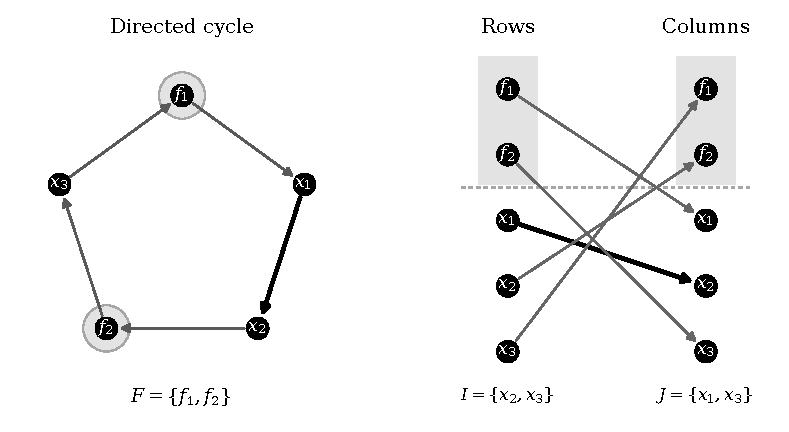
\includegraphics[width=0.94\linewidth]{figures/nonprincipal_matching.pdf}
\caption{一个永久式项中的有向五圈及其行列匹配。灰色顶点组成异常集 \(F=\{f_1,f_2\}\)。跨块边占用核心行 \(I=\{x_2,x_3\}\) 和核心列 \(J=\{x_1,x_3\}\)，留下粗边所示的非主子矩阵项 \(A[x_1,x_2]\)。图中只画出这个永久式项的边。}
\label{fig:nonprincipal_matching}
\end{figure}

下面假设 \(V(T)<16n^2\log n\)。定义异常集

\[F=\left\{i:\frac{d_i^+}{n-1}\notin[1/20,19/20]\right\},
\qquad f=|F|,\qquad M=T-F,\qquad N=n-f.\]

每个异常顶点向 \(V(T)\) 贡献至少某个固定正倍数的 \(n^2\)，故 \(f=O(\log n)\)。非异常顶点的原度差绝对值至多为 \(0.9(n-1)\)；删去 \(F\) 改变它至多 \(f\)。因此，对所有充分大的 \(n\) 一致有

\[\max_i|(S_M\mathbf1)_i/(N-1)|<0.95,\qquad
\tau_M=O(\log n).\]

对度差平方和，使用 \(\|S_M\mathbf1\|_2\le\|S\mathbf1\|_2+f\sqrt N\)，再除以 \(N-1\)。进一步删除短核心子集后，同一论证仍然适用。在这些删除中始终保留原异常集 \(F\)，因此常数可以统一选取。

先按圈覆盖在 \(F\) 与核心 \(M\) 之间的连接方式估计 \(\operatorname{per}A_T\)。异常顶点在某个方向上的邻居很少。圈覆盖需要使用两个方向的边，除非将该顶点匹配到 \(F\) 内部；后一种选择会产生 \(1/N\) 量级的代价。使用引理 4.4 的核心成对权重 \(\ell,r\)，它们的总偏移满足

\[\sum_{i\in M}|\ell_i-1|+\sum_{i\in M}|r_i-1|
\le K\sqrt{N\log n}.\]

对 \(x\in F\)，记 \(q_x=N^{-1}|\{j\in M:x\to j\}|\)。它到 \([0,1/20]\cup[19/20,1]\) 的距离为 \(O(f/n)\)。两侧带权跨边邻居之和分别由 \(N(q_x+\beta)\) 和 \(N(1-q_x+\beta)\) 控制，其中 \(\beta=O(\sqrt{\log n/n})\)。置

\[u_x=2(q_x+\beta),\qquad v_x=2(1-q_x+\beta).\]

可对全部 \(x\) 统一选取

\[u_xv_x\le c_n=19/100+o(1),\qquad
u_x,v_x\le L_n=2+o(1).\]

按排列在 \(F\) 内部使用的边分解永久式。若内部有 \(s\) 条边，其行集 \(R\) 和列集 \(C\) 均有 \(s\) 个点；每个跨边方向恰有 \(t=f-s\) 条边。核心行、列删集 \(I,J\) 均有 \(t\) 个点，但不必相同。精确四块展开为

\[\operatorname{per}A_T
=\sum_{s=0}^{f}
\sum_{\substack{R,C\subseteq F\\|R|=|C|=s}}
\sum_{\substack{I,J\subseteq M\\|I|=|J|=f-s}}
\operatorname{per}A[R,C]\,
\operatorname{per}A[F\setminus R,J]\,
\operatorname{per}A[I,F\setminus C]\,
\operatorname{per}A[M\setminus I,M\setminus J].\]

每个有贡献的排列被唯一分类。先对核心永久式使用引理 4.4 的一致上界，再分离两个跨边求和。删除核心行产生 \(\ell_i\)，删除核心列产生 \(r_j\)。固定 \(R,C\)，向外跨边求和精确等于

\[\begin{aligned}
&\sum_{\substack{J\subseteq M\\|J|=t}}
\operatorname{per}A[F\setminus R,J]\prod_{j\in J}r_j\\
&=\sum_{\phi:F\setminus R\hookrightarrow M}
\prod_{x\in F\setminus R}A_{x,\phi(x)}r_{\phi(x)}
\le\prod_{x\in F\setminus R}\sum_{j\in M}A_{xj}r_j.
\end{aligned}\]

独立地，向内跨边求和为

\[\begin{aligned}
&\sum_{\substack{I\subseteq M\\|I|=t}}
\operatorname{per}A[I,F\setminus C]\prod_{i\in I}\ell_i\\
&=\sum_{\psi:F\setminus C\hookrightarrow M}
\prod_{y\in F\setminus C}A_{\psi(y),y}\ell_{\psi(y)}
\le\prod_{y\in F\setminus C}\sum_{i\in M}A_{iy}\ell_i.
\end{aligned}\]

其中 \(\hookrightarrow\) 表示单射。每个单射由其像集及相应永久式项恰好计数一次，没有额外的 \(t!\) 因子。像集 \(I,J\) 不必相等，也不必不交，因为它们分别属于核心的行、列副本。所有因子非负，故可去掉单射限制。两个上界的乘积为

\[N^{2t}2^{-2t}
\left(\prod_{x\notin R}u_x\right)
\left(\prod_{y\notin C}v_y\right).\]

异常内部永久式至多为 \(s!\)。除以 \(n!/2^n\) 后，阶乘与二的幂合并为

\[2^sN^{2t}\frac{(N-t)!}{(N+f)!}
=\left(\frac2N\right)^s\exp(O(f^2/N)).\]

这里 \(N+f-(N-t)=f+t=2f-s\)，故阶乘比贡献 \(N^{-(2f-s)}\exp(O(f^2/N))\)，再乘 \(N^{2t}\) 后恰留下 \(N^{-s}\)。

令 \(h=|R\cap C|\)。成对乘积满足

\[\left(\prod_{x\notin R}u_x\right)
\left(\prod_{y\notin C}v_y\right)
\le c_n^{f-2s}L_n^{2s}(c_n/L_n^2)^h
\le c_n^{f-2s}L_n^{2s}.\]

第一个不等式由分别统计出现两个、一个及零个因子的顶点数得到；即使 \(f-2s\) 为负，它仍正确。引理 4.4 的误差在 \(t\le f=O(\log n)\) 内统一为 \(o(1)\)，其因子 \(\Gamma\le1\) 可舍去。由 \(\binom fs^2s!\le f^{2s}/s!\)，求和可得

\[\frac{\operatorname{per}A_T}{n!/2^n}
\le(1+o(1))e^{-1}D_N(S_M)c_n^f
\exp(O(f^2/N))
\exp\left(\frac{2L_n^2f^2}{c_n^2N}\right).\]

其中额外指数均为 \(o(1)\)。具体地，删除短核心子集 \(U\) 后，核心阶数为 \(N'=n-f-|U|\sim n\)（即 \(N'/n\to1\)），异常集合仍取原来的 \(F\)。核心的归一化度差最终仍不超过 \(0.95\)，归一化度差平方和为 \(O(\log n)\)，而跨边删集大小为 \(t\le f=O(\log n)\)。因此引理 4.4 中的误差指数为

\[O\!\left(\frac{(\log n)^{3/2}}{\sqrt n}+\frac{(\log n)^2}{n}\right)=o(1),\]

其中常数与 \(U,I,J\) 无关。跨边邻点比例相较于原始全图仅改变 \(O((f+|U|)/n)\)，权重的一范数位移仍为 \(O(\sqrt{n\log n})\)，故前述跨边求和估计也一致成立。此时核心高斯因子改变为原来的 \(\exp(O(|U|/n))\) 倍：对 \(S_M/N\) 使用高斯删行列引理，对数损失为 \(O(|U|/n)\)；将归一化尺度从 \(N\) 改为 \(N-|U|\) 也产生同阶误差。

在路径卷积中，大小为 \(k\) 且与 \(F\) 相交的子集占比至多为 \(fk/n\)。通用永久式界因而使其全部归一化短项贡献至多为

\[K\frac f{\sqrt n}\sum_k kw_k=o(1).\]

对包含于核心的子集，恢复下降阶乘后，对正主子式求和。任意核心阶数 \(N\le n\) 均满足由秩一行列式恒等式给出的界

\[\det\left(I_N+\frac2n(I_N+A_M)\right)
\le2e\det(I_N+S_M/N).\]

证明时先提出 \((1+1/n)^N\le e\)。剩余全一秩一因子至多为 \(1+N/(n+1)<2\)，因为 \(I+S_M/(n+1)\) 的逆矩阵的实二次型至多为向量范数的平方。最后，反对称频率行列式乘积在尺度从 \(1/(n+1)\) 增至 \(1/N\) 时单调增大。

短子集的下降阶乘恢复带来 \(\exp(O(k_n^2/n))=1+o(1)\)。由于最终 \(c_n<1/4\)，上述统一估计给出

\[\frac{H(T)}{\mu_n}
\le(1/4)^f\rho_N(S_M)+o(1)
\le C_*/4+o(1)<1,\qquad f\ge1.\]

由于 \(P(n)\ge\mu_n\)，充分大阶数时，含异常顶点的图不能达到最大路径数。还可将上界放宽为 \((10/3)4^{-f}(1+\varepsilon_n)\)：这里计入的是删集与 \(F\) 不相交的短卷积项；其余短项和长项合计记为 \(\delta_n\)。于是

\stepcounter{equation}

\begin{equation}
\frac{H(T)}{\mu_n}\le\frac{10}{3}4^{-f}(1+\varepsilon_n)+\delta_n,
\qquad \varepsilon_n,\delta_n\longrightarrow0.
\tag{7.1}
\label{eq-exceptional-bound}
\end{equation}

两个误差均在上述低方差图类上一致趋于零。取 \(n\) 充分大，使 \(1+\varepsilon_n\le21/20\)，并使与 \(F\) 相交的短项及长项各不超过 \(1/25\)。当 \(f\ge1\) 时，\hyperref[eq-exceptional-bound]{式 (7.1)}给出

\[\frac{10}{3}\cdot\frac14\cdot\frac{21}{20}+\frac1{25}+\frac1{25}
=\frac{191}{200}<1.\]

两种选择均不影响最终上界常数。

异常点满足

\[|d_i^+-(n-1)/2|>\frac9{20}(n-1),\quad
f\frac{81}{400}(n-1)^2\le V(T)<16n^2\log n,\]

故 \(f<(6400/81)(n/(n-1))^2\log n\)。对核心，

\[\max_i|s_i^M|\le0.9(n-1)+f,
\quad \frac{0.9(n-1)+f}{n-f-1}\longrightarrow0.9,\]

\[\tau_M\le\frac{2\|s\|_2^2+2f^2N}{(N-1)^2}
=O(\log n)+O((\log n)^2/n)=O(\log n).\]

因为 \(|\ell_i-1|\le|a_i|/(1-b)\)、\(|r_i-1|\le|a_i|/(1-b)\)，

\[\sum_i(|\ell_i-1|+|r_i-1|)
\le\frac2{1-b}\sum_i|a_i|
\le\frac2{1-b}\sqrt{N\tau_M}=O(\sqrt{N\log n}).\]

这使任意邻居子集的加权计数与普通计数相差至多上述总偏移。具体地，

\[\sum_jA_{xj}r_j\le Nq_x+K\sqrt{N\log n},\quad
\sum_iA_{ix}\ell_i\le N(1-q_x)+K\sqrt{N\log n}.\]

当 \(q\in[0,1/20]\cup[19/20,1]\) 时，\(4q(1-q)\le4(1/20)(19/20)=19/100\)；邻居比例的 \(O(f/n)\) 扰动与 \(\beta=o(1)\) 扰动共同给出 \(u_xv_x\le19/100+o(1)\)。

四块展开中 \(t=f-s\)；依次取异常内部 \(s\) 条边、异常到核心 \(t\) 条边、核心到异常 \(t\) 条边、核心内部 \(N-t\) 条边，总数

\[s+t+t+(N-t)=N+f=n.\]

永久式展开没有符号，分类后每个排列只出现一次。全部二次幂及阶乘因子为

\[\frac{[(N-t)!/2^{N-t}]\,[N^{2t}/2^{2t}]}{(N+f)!/2^{N+f}}
=2^{f-t}N^{2t}\frac{(N-t)!}{(N+f)!}
=2^sN^{2t}\frac{(N-t)!}{(N+f)!}.\]

由于

\[\frac{(N-t)!}{(N+f)!}=\prod_{h=-t+1}^{f}\frac1{N+h}
=N^{-(f+t)}\exp\left(-\sum_{h=-t+1}^{f}\log(1+h/N)\right),\]

且 \(\sum|h|/N=O(f^2/N)\)，上式变为

\[2^sN^{2t-(f+t)}e^{O(f^2/N)}=(2/N)^se^{O(f^2/N)}.\]

若 \(h=|R\cap C|\)，同时出现 \(u,v\) 两因子的顶点数为 \(f-2s+h\)，只出现一个因子的顶点数为 \(2s-2h\)；于是

\[c_n^{f-2s+h}L_n^{2s-2h}
=c_n^{f-2s}L_n^{2s}(c_n/L_n^2)^h
\le c_n^{f-2s}L_n^{2s}.\]

全部内部边选择的求和为

\[\begin{aligned}
\sum_{s=0}^f\binom fs^2s!(2/N)^sc_n^{f-2s}L_n^{2s}
&\le c_n^f\sum_{s=0}^f\frac1{s!}
\left(\frac{2L_n^2f^2}{c_n^2N}\right)^s\\
&\le c_n^f\exp\left(\frac{2L_n^2f^2}{c_n^2N}\right).
\end{aligned}\]

以下 \(\#E\) 与 \(|E|\) 均表示有限集合 \(E\) 的元素数。\(k=0\) 时删集不与异常集相交，所占比例为零；对 \(1\le k\le n\)，该比例满足

\[\frac{\#\{U:|U|=k,U\cap F\ne\varnothing\}}{\binom nk}
\le\sum_{x\in F}\frac{\binom{n-1}{k-1}}{\binom nk}=fk/n.\]

乘通用卷积权重 \(K\sqrt n\,w_k\) 后总和为 \(Kf\sum_kkw_k/\sqrt n=o(1)\)。

令 \(Q=S_M/(n+1)\)，\(v=\mathbf1_N\)，则

\[\begin{aligned}
\det\left(I_N+\frac2n(I_N+A_M)\right)
&=(1+1/n)^N\det(I_N+Q)
\left[1+\frac1{n+1}v^{\mathsf T}(I_N+Q)^{-1}v\right].
\end{aligned}\]

利用 \((I+Q)^{-1}=(I-Q)(I-Q^2)^{-1}\) 及反对称二次型为零，

\[v^{\mathsf T}(I+Q)^{-1}v=v^{\mathsf T}(I+Q^{\mathsf T}Q)^{-1}v\le\|v\|_2^2=N.\]

又 \((1+1/n)^N\le e^{N/n}\le e\)，并且

\[\det(I+S_M/(n+1))=\prod_j\left(1+\frac{\lambda_j^2}{(n+1)^2}\right)
\le\prod_j\left(1+\frac{\lambda_j^2}{N^2}\right).\]

三项分别由 \(e\)、\(\det(I+S_M/N)\) 和 \(2\) 控制。再乘永久式中的 \(e^{-1}/2\)，得到 \(\rho_N(S_M)\)。上述异常集估计中的常数满足

\[\frac{10}{3}\frac14\frac{21}{20}=\frac78=\frac{175}{200},\qquad
\frac1{25}+\frac1{25}=\frac{16}{200},\qquad
\frac{175+16}{200}=\frac{191}{200}.\]

设删去异常点和短集后，每个异常点的核心邻居比例距 \([0,1/20]\cup[19/20,1]\) 至多为 \(\epsilon_n\)，其中 \(\epsilon_n=O((f+k_n)/n)\)。对 \(q\in[0,1]\)，函数 \(q(1-q)\) 的导数绝对值至多一。因此

\[q_x(1-q_x)\le\frac{19}{400}+\epsilon_n.\]

用同一个非负权重偏移 \(\beta_n=O(\sqrt{\log n/n})\)，

\[\begin{aligned}
u_xv_x
&=4(q_x+\beta_n)(1-q_x+\beta_n)\\
&=4q_x(1-q_x)+4\beta_n+4\beta_n^2\\
&\le\frac{19}{100}+4\epsilon_n+4\beta_n+4\beta_n^2=:c_n.
\end{aligned}\]

而 \(u_x,v_x\le2+2\beta_n=:L_n\)。因 \(\epsilon_n,\beta_n\to0\)，可先选统一阈值使

\[4\epsilon_n+4\beta_n+4\beta_n^2<\frac6{100},\qquad c_n<\frac14.\]

上述额外指数的每一项也都趋于零：

\[\frac{f^2}{N}=O((\log n)^2/n)\to0,
\quad
\frac{2L_n^2f^2}{c_n^2N}=O((\log n)^2/n)\to0.\]

引理 4.4 的误差项在 \(\tau\le A\log n,t\le B\log n\) 时分别至多为常数乘

\[\frac{\log n+(\log n)^2}{n},\quad
\frac{(\log n)^{3/2}}{\sqrt n},\quad
\sqrt{\frac{\log n}{n}},\quad
\frac{\log n+1}{n},\quad
\frac{(\log n)^{3/2}}{\sqrt n},\quad
\frac{(\log n)^2}{n}.\]

上述常数均与竞赛图及删集无关，故所得 \(o(1)\) 误差也是一致的。

\Needspace{5\baselineskip}
\subsection{7.4 剩余图类中的度差修正因子}\label{ux5269ux4f59ux56feux7c7bux4e2dux7684ux5ea6ux5deeux4feeux6b63ux56e0ux5b50}

剩余竞赛图满足

\[\max_i|a_i|\le0.9,\qquad
a=s/(n-1),\qquad \tau=\sum_i a_i^2\le K\log n.\]

以下固定一个绝对常数 \(K_0\)，使 \(\tau\le K_0\log n\)。其成对乘积满足

\[\Gamma=\prod_i(1-a_i^2)\le e^{-\tau}.\]

现在对整个竞赛图应用引理 4.4。度差乘积是所有短项共有的因子；将它保持在总和之外，可以吸收那些单独看来比 \(1/n\) 更大的误差。

对大小为 \(k\le k_n\) 的主删集 \(U\)，引理 4.4 给出

\[\operatorname{per}A[U^c]\le
e^{-1}D_n(S)\Gamma
\left(\prod_{i\in U}g_i\right)
\frac{(n-k)!}{2^{n-k}}\exp(R_\tau+R_{\tau,k}),\]

\[g_i=(1-a_i^2)^{-1}\le G:=100/19,\]

\[R_\tau\le K[\mathcal M_\tau+\sqrt{\tau/n}+1/n],\qquad
R_{\tau,k}\le K[k\sqrt{\tau/n}+(k+k^2)/n].\]

在累计误差时，必须保留公共因子 \(\Gamma\)。定义非负系数

\[c_k=(2/n)^k\sum_{|U|=k}\det(I+A[U])\prod_{i\in U}g_i.\]

它们满足 \(c_0=1\)、\(c_k\le G^kw_k\)。下降阶乘的恢复产生

\[\log\frac{n^k}{(n)_k}=O(k^2/n),\qquad k\le k_n.\]

令 \(\delta_n=\sqrt{\tau/n}+1/n\)，\(r_k=R_{\tau,k}+\log(n^k/(n)_k)\)。将误差上界选为非负值后，对 \(\tau\le K_0\log n\) 一致有 \(0\le r_k\le K\delta_n(k+k^2)\)，且 \(\max_{k\le k_n}r_k=o(1)\)。因此

\[\sum_{k\le k_n}c_ke^{r_k}
\le\sum_{k=0}^{n}c_k+
K\delta_n\sum_{k\ge0}G^kw_k(k+k^2)
\le\left(\sum_{k=0}^{n}c_k\right)e^{K\delta_n}.\]

最后一步使用 \(\sum_kc_k\ge1\) 以及相应固定矩的收敛性。归一化短路径总和因而至多为

\[\frac{e^{-1}D_n(S)\Gamma}{2}
e^{R_\tau+K\delta_n}
\det\left(I+\frac2n\operatorname{diag}(g)(I+A)\right).\]

误差总和由 \(G^kw_k\) 的有限矩控制，而非由最大删集大小 \(k_n\) 控制。这避免了在最终误差中引入额外的对数因子。

下面去除权重，同时保持度差修正因子。令 \(W=I+(2/n)(I+A)\)、\(\Delta=(2/n)\operatorname{diag}(g-1)(I+A)\)。\(W\) 的对称部分至少为 \(I\)，故 \(\|W^{-1}\|_{\rm op}\le1\)。由于 \(I+A\) 每行的二范数至多为 \(\sqrt n\)，且 \(\sum_i(g_i-1)\le K\tau\)，将 \(\Delta\) 分解为秩一行矩阵之和，可以控制其迹范数，即奇异值之和。由 \(\|uv^{\mathsf T}\|_*=\|u\|_2\|v\|_2\)，得到

\[\|\Delta\|_*\le K\tau/\sqrt n.\]

由行列式不等式 \(|\det(I+E)|\le\exp(\|E\|_*)\)，可得

\[\det(W+\Delta)\le\det(W)e^{K\tau/\sqrt n}.\]

两个行列式均为正：\(W\) 的对称部分正定；加权行列式的主子式展开系数为正。第 7.3 节的无权秩一界在 \(N=n\) 时为 \(\det(W)\le2e\det(I+S/n)\)。

合并上述各因子，最后仅加入长删集尾项，得到保留度差修正因子的一致上界

\stepcounter{equation}

\begin{equation}
\frac{H(T)}{\mu_n}\le
\rho_n(S)\exp\left\{-\tau+
K\left[\frac{1+\tau+\tau^2}{n}
+\frac{\tau^{3/2}+\tau}{\sqrt n}+\sqrt{\tau/n}\right]\right\}
+o(1/n).
\tag{7.2}
\label{eq-score-penalty}
\end{equation}

当 \(\tau\le K_0\log n\) 时，除常数 \(1/n\) 外的多项式误差项，在充分大阶数总共至多消耗 \(\tau/4\)。剩余平方根项由 Young 不等式控制：

\[K\sqrt{\tau/n}\le\tau/4+K^2/n.\]

\hyperref[eq-score-penalty]{式 (7.2)}中的总指数因此至多为 \(-\tau/2+K/n\)。再使用谱上限，得到

\[H(T)/\mu_n\le C_*e^{K/n}+o(1/n)=C_*+O(1/n).\]

由 \(g_i-1=a_i^2/(1-a_i^2)\)，

\[\sum_i(g_i-1)\le\frac{\tau}{1-0.9^2}=\frac{100}{19}\tau,
\qquad
c_k\le(2/n)^k\binom nk h_kG^k\le G^kw_k.\]

对于 \(k\le k_n=o(\sqrt n)\)，

\[0\le\log\frac{n^k}{(n)_k}
=\sum_{h=0}^{k-1}-\log(1-h/n)
\le\frac{k(k-1)}{2n(1-k_n/n)}\le Kk^2/n.\]

当 \(0\le r_k\le1\) 时，\(e^{r_k}-1=\int_0^{r_k}e^u\,du\le er_k\)，故

\[\sum_{k\le k_n}c_k(e^{r_k}-1)
\le K\delta_n\sum_{k\ge0}G^kw_k(k+k^2)=K'\delta_n.\]

记 \(C=\sum_{k=0}^nc_k\ge1\)，则 \(C+K'\delta_n\le C(1+K'\delta_n)\le Ce^{K'\delta_n}\)。加权主子式展开逐项给出

\[\sum_{k=0}^nc_k
=\sum_U(2/n)^{|U|}\det(I+A[U])\prod_{i\in U}g_i
=\det(I+(2/n)\operatorname{diag}(g)(I+A)).\]

记 \(I+A\) 的第 \(i\) 行为 \(r_i^{\mathsf T}\)，\(e_i\) 为第 \(i\) 个标准基向量。则

\[\Delta=\frac2n\sum_i(g_i-1)e_ir_i^{\mathsf T},\quad
\|\Delta\|_*\le\frac2n\sum_i(g_i-1)\|e_i\|_2\|r_i\|_2
\le\frac2{\sqrt n}\sum_i(g_i-1)\le K\tau/\sqrt n.\]

若 \(E\) 的奇异值为 \(\sigma_j(E)\)，则

\[|\det(I+E)|\le\prod_j(1+\sigma_j(E))
\le\exp\left(\sum_j\sigma_j(E)\right)=e^{\|E\|_*}.\]

使用 \(W+\Delta=W(I+W^{-1}\Delta)\) 及 \(\|W^{-1}\|_{\rm op}\le1\) 得到所述比较。

最后令

\[E_n(\tau)=K\left[\frac{\tau+\tau^2}{n}
+\frac{\tau^{3/2}+\tau}{\sqrt n}\right].\]

当 \(0\le\tau\le K_0\log n\) 时，

\[E_n(\tau)\le\tau K\left[\frac{1+K_0\log n}{n}
+\frac{\sqrt{K_0\log n}+1}{\sqrt n}\right]\le\tau/4\]

对所有充分大 \(n\) 一致成立。配方给出

\[0\le\left(\frac{\sqrt\tau}{2}-\frac K{\sqrt n}\right)^2
=\frac\tau4-K\sqrt{\tau/n}+\frac{K^2}n,\]

所以总指数至多为 \(-\tau+\tau/4+\tau/4+(K+K^2)/n\)。又

\[0\le e^{K'/n}-1=\int_0^{K'/n}e^u\,du\le K'e^{K'}/n,\]

得到 \(C_*+O(n^{-1})\)，其中常数完全不依赖 \(\tau\) 和竞赛图。

\Needspace{5\baselineskip}
\subsection{7.5 完成上界}\label{ux5b8cux6210ux4e0aux754c}

三类图覆盖全部竞赛图。高方差图的归一化路径数为 \(o(1/n)\)；低方差但含异常点的图严格低于一；所有剩余图满足刚才的 \(C_*+O(1/n)\) 上界。因此

\[{P(n)\le\bigl(C_*+O(1/n)\bigr)\mu_n.}\]

三种情形中的起始阶数均不依赖具体竞赛图，因此取一个共同阈值便得到命题 1.1 的上界。

\Needspace{11\baselineskip}
\section{8. 小度差公式与路径下界}\label{ux5c0fux5ea6ux5deeux516cux5f0fux4e0eux8defux5f84ux4e0bux754c}

\textbf{定理 8.1（小度差路径近似）。}

存在绝对常数 \(C\)，具有如下性质：对每个满足 \(d(n)/\sqrt n\to0\) 的非负函数 \(d=d(n)\)，存在阈值 \(n_0(d)\)，使每个阶数为 \(n\ge n_0(d)\) 且 \(\|S\mathbf1\|_\infty\le d(n)\) 的竞赛图都满足

\[\left|\frac{H(T)}{\mu_n}-\rho_n(S)\right|\le C\frac{(d(n)+1)^2}{n}.\]

\Needspace{8\baselineskip}
\subsection{8.1 小度差近似的证明}\label{ux5c0fux5ea6ux5deeux8fd1ux4f3cux7684ux8bc1ux660e}

\textbf{证明。}

以下记 \(d=d(n)\)。对每个主删集 \(|U|=k\le k_n\)，应用引理 4.5。因 \(d+k_n+1=o(\sqrt n)\)，其适用性对全部这些子集一致。恢复下降阶乘 \((n)_k\) 后，由正路径卷积得到

\[\frac{H(T)}{\mu_n}
=\frac{e^{-1}D_n(S)}2
\sum_{k\le k_n}\left(\frac2n\right)^k
\sum_{|U|=k}\det(I+A[U])
+O\left(\frac{(d+1)^2}{n}\right).\]

此误差率没有额外对数因子，因为误差至多为固定常数乘上

\[\frac1n\sum_{k\ge0}w_k(d+k+1)^2
=O\left(\frac{(d+1)^2}{n}\right).\]

下降阶乘恢复误差贡献 \(O(n^{-1}\sum k^2w_k)\)；大删集对应的项由第 5.1 节控制为 \(o(n^{-1})\)。将上式短生成和扩展到全部 \(k\) 的代价为 \(n^{-2+o(1)}\)，因为系数被 \(w_k\) 控制。于是

\[\frac{H(T)}{\mu_n}
=\frac{e^{-1}D_n(S)}2
\det\left(I+\frac2n(I+A)\right)
+O\left(\frac{(d+1)^2}{n}\right).\]

令 \(u=\mathbf1/\sqrt n\)，\(Q=S/(n+1)\)。秩一行列式引理给出

\[\det\left(I+\frac2n(I+A)\right)
=(1+1/n)^n\det(I+Q)
\left(1+\frac n{n+1}u^{\mathsf T}(I+Q)^{-1}u\right).\]

反对称性给出

\[u^{\mathsf T}(I+Q)^{-1}u=u^{\mathsf T}(I-Q^2)^{-1}u,\]

该量与一的差的绝对值不超过

\[\|Qu\|_2^2\le\frac{d^2}{(n+1)^2}.\]

又有 \((1+1/n)^n=e(1+O(n^{-1}))\)；将 \(S/(n+1)\) 换为 \(S/n\) 的对数行列式误差为 \(O(n^{-1})\)，这是由归一化频率平方的有界总和得到的。因此

\[\det\left(I+\frac2n(I+A)\right)
=2e\det(I+S/n)\left(1+O(n^{-1}+d^2/n^2)\right).\]

代回即得定理。各估计使用同一个绝对常数；只有小度差条件开始成立的阶数依赖函数 \(d\)。

对每个 \(k\)，由 \(d+k+1\le(d+1)(k+1)\)，

\[\frac1n\sum_kw_k(d+k+1)^2
\le\frac{(d+1)^2}{n}\sum_kw_k(k+1)^2.\]

因此无需用 \(k_n\) 替代 \(k\)，也不会产生 \(\log n\) 损失。对 \(Q^{\mathsf T}=-Q\)，

\[(I+Q)^{-1}=(I-Q)(I-Q^2)^{-1},\qquad
Q(I-Q^2)^{-1}\text{ 为反对称矩阵},\]

\[\begin{aligned}
1-u^{\mathsf T}(I+Q)^{-1}u
&=u^{\mathsf T}[I-(I+Q^{\mathsf T}Q)^{-1}]u\\
&=(Qu)^{\mathsf T}(I+QQ^{\mathsf T})^{-1}(Qu)
\le\|Qu\|_2^2.
\end{aligned}\]

由于 \(Qu=s/[(n+1)\sqrt n]\)，

\[\|Qu\|_2^2=\frac{\sum_i s_i^2}{n(n+1)^2}\le\frac{d^2}{(n+1)^2}.\]

改变归一化尺度产生的行列式误差满足

\[\begin{aligned}
0&\le\log\det(I+S/n)-\log\det(I+S/(n+1))\\
&=\sum_j\int_{\lambda_j^2/(n+1)^2}^{\lambda_j^2/n^2}\frac{du}{1+u}\\
&\le\sum_j\lambda_j^2\left(\frac1{n^2}-\frac1{(n+1)^2}\right)\\
&=\frac{n(n-1)}2\frac{2n+1}{n^2(n+1)^2}=O(n^{-1}).
\end{aligned}\]

且

\[0\le1-n\log(1+1/n)
=n\int_0^{1/n}\frac{u}{1+u}\,du\le\frac1{2n}.\]

秩一因子与二的差为

\[\left|1+\frac n{n+1}u^{\mathsf T}(I+Q)^{-1}u-2\right|
\le\frac1{n+1}+\frac{d^2}{(n+1)^2}.\]

依次相乘并用 \(D_n(S)\det(I+S/n)\le C_*\)，即得到定理 8.1 的绝对误差。 \(\square\)

\Needspace{20\baselineskip}
\subsection{8.2 圆环竞赛图}\label{ux5706ux73afux7adeux8d5bux56fe}

\begin{figure}[htbp]
\centering
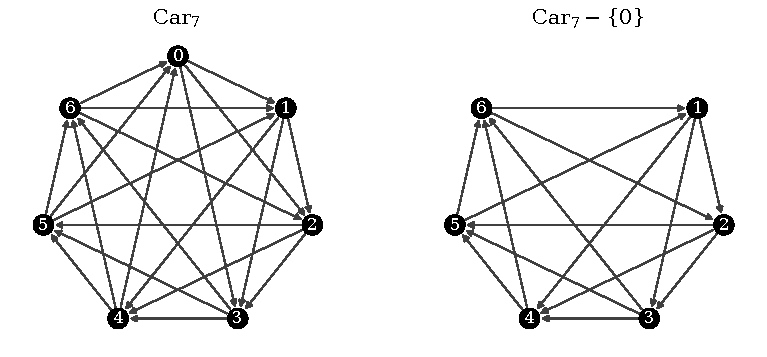
\includegraphics[width=0.94\linewidth]{figures/carousel_deletion.pdf}
\caption{圆环图 \(\mathrm{Car}_7\) 及删除顶点 \(0\) 后的偶阶图。左图每个顶点的出度均为 \(3\)；右图各顶点的出度为 \(2\) 或 \(3\)。两图均画出全部边。}
\label{fig:carousel_deletion}
\end{figure}

\Needspace{7\baselineskip}
\textbf{推论 8.2（圆环图下界）。}

对下面定义的奇阶圆环图及偶阶一点删除构造，

\[H(\mathrm{Car}_n)/\mu_n=L+O(n^{-1}).\]

\Needspace{4\baselineskip}
\textbf{证明。}

对奇数 \(n\)，在模 \(n\) 的剩余类上定义圆环竞赛图 \(\mathrm{Car}_n\)：当 \(1\le j\le(n-1)/2\) 时，令 \(i\to i+j\)。该图正则，故 \(d=0\)。对偶数 \(n\)，令 \(\mathrm{Car}_n\) 为 \(\mathrm{Car}_{n+1}\) 删去一个顶点所得的图，此时 \(d=1\)。

奇阶圆环符号矩阵与 \(T_n^0\) 带符号置换相似。一个显式构造是：用对角符号 \((-1)^i\)，\(0\le i<n\)，共轭 \(T_n^0\)，再按 \(0,2,\ldots,n-1,1,3,\ldots,n-2\) 重排指标；两个指标同奇偶时，切换后的边沿指标递增方向；异奇偶时方向相反。按上述循环顺序读取指标，即得到圆环方向。将逆向的带符号共轭和重排限制到偶阶的一点删除后，变换所得的矩阵为剩余有序指标上的 \(T_n^0\)。因此，删除任意一个顶点后，同一带符号谱计算仍然适用，奇偶两类均满足

\[\rho_n(S_{\mathrm{Car}_n})
=r_n:=\frac{(n+1)^n+(n-1)^n}{(n+i)^n+(n-i)^n}.\]

分子、分母均除以 \(n^n\)，并对四个固定值 \(z=1,-1,i,-i\) 使用 \((1+z/n)^n\) 的 Taylor 展开，得到

\[r_n=\frac{\cosh1}{\cos1}+O(n^{-1})=L+O(n^{-1}).\]

故奇偶两类都有 \(H(\mathrm{Car}_n)/\mu_n=L+O(n^{-1})\)，于是

\[P(n)\ge(L-O(n^{-1}))\mu_n.\]

从带符号相似过渡到路径数，使用的是定理 8.1，分别对应 \(d=0\) 和 \(d=1\)。设下界与上界的常数和阈值分别为 \(K_l,N_l\) 与 \(K_u,N_u\)。取 \(K=K_l+K_u\)、\(n_0=\max(N_l,N_u,2)\)，即得命题 1.1。

写 \(n=2m+1\)，原指标 \(i=0,\ldots,2m\)。令 \(D_{ii}=(-1)^i\)，则对 \(i<j\)，

\[(DT_n^0D)_{ij}=(-1)^{i+j}.\]

取重排 \(p_k=2k\pmod n\)（取 \(0,\ldots,n-1\) 的代表元），它依次为 \(0,2,\ldots,2m,1,3,\ldots,2m-1\)。若 \(i,j\) 同奇偶，正向差为偶数 \(2h\)，则

\[2^{-1}(j-i)\pmod n=h\in\{1,\ldots,m\}.\]

若异奇偶且 \(i<j\)，写 \(j-i=2h+1\)，则

\[2^{-1}(j-i)\pmod n=h+m+1\in\{m+1,\ldots,2m\}.\]

所以在新指标下，差 \(1,\ldots,m\) 的边顺向，差 \(m+1,\ldots,2m\) 的边逆向，正好是圆环图。删一点时取对应主子矩阵；限制后的 \(D\) 仍为符号对角矩阵，而传递矩阵在保留有序指标上的主子矩阵仍为 \(T_n^0\)。这证明奇偶构造都具有上述谱，不声称带符号变换保持路径数。

由 \(D_n(S)=\det(I+iS/n)^{-1}\) 及主子式多项式，

\[\begin{aligned}
\rho_n(S)&=\frac{\det(I+S/n)}{\det(I+iS/n)}\\
&=\frac{(1+1/n)^n+(1-1/n)^n}
{(1+i/n)^n+(1-i/n)^n}=r_n.
\end{aligned}\]

对 \(z\in\{1,-1,i,-i\}\)、\(n\ge2\)，在主值对数的 \(|w|<1\) 级数中，

\[\begin{aligned}
n\log(1+z/n)&=z-\frac{z^2}{2n}+R_{n,z},\\
|R_{n,z}|&\le\sum_{h=3}^{\infty}\frac1{h n^{h-1}}
\le\frac1{3n^2(1-1/n)}\le\frac2{3n^2}.
\end{aligned}\]

指数化得 \((1+z/n)^n=e^z(1-z^2/(2n)+O(n^{-2}))\)。分别相加：

\[\begin{aligned}
(1+1/n)^n+(1-1/n)^n&=2\cosh1\,[1-1/(2n)+O(n^{-2})],\\
(1+i/n)^n+(1-i/n)^n&=2\cos1\,[1+1/(2n)+O(n^{-2})].
\end{aligned}\]

因为 \(\cos1>0\)，分母对充分大 \(n\) 有固定正下界。利用

\[\frac1{1+u}=1-u+\frac{u^2}{1+u},\]

得到更精细的谱比值

\[r_n=L[1-1/n+O(n^{-2})].\]

定理 8.1 对路径数本身只给 \(O(n^{-1})\) 误差，故这里的 \(-L/n\) 只能称为谱比值的修正项，不能直接当作路径数的修正项。最后

\[H(\mathrm{Car}_n)/\mu_n=r_n+O(n^{-1})=L+O(n^{-1}),\]

从而存在固定 \(K_l\) 使 \(P(n)\ge(L-K_l/n)\mu_n\)。 \(\square\)

\Needspace{5\baselineskip}
\section{A. 标准工具的展开证明}\label{a.-ux6807ux51c6ux5de5ux5177ux7684ux5c55ux5f00ux8bc1ux660e}

本附录给出正文所用标准估计的证明。

\Needspace{5\baselineskip}
\subsection{A.1 行列式工具}\label{a.1-ux884cux5217ux5f0fux5de5ux5177}

\textbf{主子式展开。} 对 \(I+tM\) 的第 \(j\) 列，选单位列 \(e_j\) 或矩阵列 \(tM_{\cdot j}\)。行列式的多线性给出 \(2^n\) 个选择。若选矩阵列的指标为 \(U\)，沿其余单位列展开，剩下 \(M[U]\)，符号为正。因此

\[\det(I+tM)=\sum_{U\subseteq[n]}t^{|U|}\det M[U].\]

\textbf{秩一引理。} 对向量 \(a,b\)，矩阵 \(ab^{\mathsf T}\) 的任意两列线性相关，所以上式在 \(M=ab^{\mathsf T}\) 时只有零阶、一阶项：

\[\det(I+ab^{\mathsf T})=1+\sum_i a_ib_i=1+b^{\mathsf T}a.\]

若 \(M\) 可逆，则

\[\det(M+ab^{\mathsf T})=\det M\det(I+M^{-1}ab^{\mathsf T})
=\det M(1+b^{\mathsf T}M^{-1}a).\]

\textbf{Hadamard 不等式。} 对矩阵的行向量 \(r_1,\ldots,r_n\) 做 Gram--Schmidt 正交化，得到正交向量 \(q_1,\ldots,q_n\)。减去前面行的线性组合不改变行列式，所以

\[|\det M|^2=\det(MM^*)=\prod_i\|q_i\|_2^2
\le\prod_i\|r_i\|_2^2.\]

行相关时两侧仍成立，因为左侧为零。开平方得 \(|\det M|\le\prod_i\|r_i\|_2\)。

后面还使用行列式微分。先对一个小矩阵扰动 \(K\) 使用主子式展开：

\[\det(I+K)=1+\operatorname{tr}K+
\sum_{\substack{U\subseteq[p]\\|U|\ge2}}\det K[U]
=1+\operatorname{tr}K+O(\|K\|_F^2),\qquad K\to0.\]

最后一个余项可以直接逐项估计。记 \(\delta=\|K\|_F\le1\)，则每个元素满足 \(|K_{ij}|\le\delta\)。若 \(|U|=r\ge2\)，由行列式的排列定义，

\[|\det K[U]|
\le\sum_{\pi\in \mathfrak S_r}\prod_{i=1}^r|K[U]_{i,\pi(i)}|
\le r!\delta^r\le r!\delta^2.\]

因此固定阶数 \(p\) 时，令 \(C_p=\sum_{r=2}^p\binom pr r!\)（\(p=1\) 时为空和零），就有

\[\left|\det(I+K)-1-\operatorname{tr}K\right|
\le\sum_{r=2}^p\binom pr r!\delta^2=C_p\|K\|_F^2.\]

这里 \(C_p\) 允许依赖阶数。若矩阵函数 \(M\) 在 \(t\) 处可微，且 \(M(t)\) 可逆，则

\[M(t+h)=M(t)+hM'(t)+R(h),\qquad
\|R(h)\|_F=o(|h|).\]

以下只需 \(R(h)=o(h)\)。令

\[K(h)=hM(t)^{-1}M'(t)+M(t)^{-1}R(h).\]

由 \(M(t)^{-1}\) 是固定矩阵，逐项得到

\[\|M(t)^{-1}R(h)\|_F
\le\|M(t)^{-1}\|_{\rm op}\|R(h)\|_F=o(|h|),
\qquad \|K(h)\|_F=O(|h|).\]

再提出 \(M(t)\) 并展开行列式：

\[\begin{aligned}
\det M(t+h)
&=\det M(t)\det(I+K(h))\\
&=\det M(t)\left[1+\operatorname{tr}K(h)+O(\|K(h)\|_F^2)\right]\\
&=\det M(t)\left[
1+h\operatorname{tr}(M(t)^{-1}M'(t))+o(|h|)\right].
\end{aligned}\]

第三行中的余项满足

\[\begin{aligned}
\left|\operatorname{tr}(M(t)^{-1}R(h))\right|
&\le\sqrt p\,\|M(t)^{-1}R(h)\|_F=o(|h|),\\
C_p\|K(h)\|_F^2&=O(h^2)=o(|h|).
\end{aligned}\]

第一个不等式是对 \(p\) 个对角元使用 Cauchy--Schwarz；第二行使用 \(h^2/|h|=|h|\to0\)。

减去 \(\det M(t)\)、除以 \(h\ne0\)，再令 \(h\to0\)，得到

\[\frac{d}{dt}\det M(t)
=\det M(t)\operatorname{tr}[M(t)^{-1}M'(t)].\]

若实矩阵路径在所讨论区间上满足 \(\det M(t)>0\)，才可直接取实对数。此时链式法则给出

\[\frac{d}{dt}\log\det M(t)
=\frac{(\det M(t))'}{\det M(t)}
=\operatorname{tr}[M(t)^{-1}M'(t)].\]

正文的 Gram 比较使用 \(M(t)=I-H(t)>0\)，确实满足这个条件。形式级数部分则使用常数项为一的行列式及其形式对数，不假定任意复数都有统一的对数分支。

一个一阶反例说明可微与二阶余项的区别：令 \(M(t)\) 是一阶矩阵 \([1+|t|^{3/2}]\)。在 \(t=0\) 处，

\[M'(0)=\lim_{h\to0}\frac{|h|^{3/2}}h=0,
\qquad
\frac{|M(h)-M(0)-hM'(0)|}{h^2}=|h|^{-1/2}\longrightarrow\infty.\]

因此，可微并不足以保证二阶余项；正文所用的线性矩阵路径则满足上述微分公式的条件。

\Needspace{5\baselineskip}
\subsection{A.2 矩阵范数工具}\label{a.2-ux77e9ux9635ux8303ux6570ux5de5ux5177}

向量二范数为 \(\|x\|_2=(\sum_i|x_i|^2)^{1/2}\)。当 \(y=0\) 时 \(|x^*y|\le\|x\|_2\|y\|_2\) 直接成立。当 \(y\ne0\) 时取复标量 \(c=(y^*x)/\|y\|_2^2\)，逐项展开

\[0\le\|x-cy\|_2^2
=\|x\|_2^2-cx^*y-\overline c\,y^*x+|c|^2\|y\|_2^2
=\|x\|_2^2-\frac{|y^*x|^2}{\|y\|_2^2}.\]

乘 \(\|y\|_2^2\)、开非负平方根，得到复数情形的 Cauchy--Schwarz：\(|x^*y|\le\|x\|_2\|y\|_2\)。

矩阵算子范数测量最大伸长倍数：

\[\|M\|_{\rm op}=\max_{\|x\|_2=1}\|Mx\|_2.\]

Frobenius 范数将矩阵看作一个长向量：

\[\|M\|_F^2=\sum_{ij}|M_{ij}|^2=\operatorname{tr}(M^*M).\]

迹 \(\operatorname{tr}M\) 就是对角元之和。交换两个相容矩阵的顺序不改变乘积的迹，因为

\[\operatorname{tr}(AB)=\sum_i\sum_jA_{ij}B_{ji}
=\sum_j\sum_iB_{ji}A_{ij}=\operatorname{tr}(BA).\]

这是后面在行侧和列侧 Gram 矩阵之间交换表达式时使用的基本有限求和规则。

因为 \(M^*M\) 是 Hermitian 半正定矩阵，它可酉对角化，特征值非负。设这些特征值为 \(s_i^2\)，\(s_i\ge0\) 称奇异值，则

\[\|M\|_{\rm op}=\max_i s_i,\qquad \|M\|_F^2=\sum_i s_i^2.\]

若 \(M^*Mv_i=s_i^2v_i\) 且 \(s_i>0\)，令 \(u_i=Mv_i/s_i\)，则

\[u_i^*u_j=\frac{v_i^*M^*Mv_j}{s_is_j}=\mathbf1\{i=j\}.\]

补齐正交基后得到 \(M=U\operatorname{diag}(s_i)V^*\)，即奇异值分解。由此定义迹范数 \(\|M\|_*=\sum_i s_i\)，并有

\[\|M\|_{\rm op}\le\|M\|_F\le\|M\|_*,\qquad
\sum_i s_i\le\sqrt n\left(\sum_i s_i^2\right)^{1/2}.\]

当 \(a,b\) 均非零时，秩一矩阵 \(ab^*\) 的唯一非零奇异值为 \(\|a\|\|b\|\)，因为

\[(ab^*)^*(ab^*)=\|a\|^2bb^*.\]

若 \(a=0\) 或 \(b=0\)，矩阵为零，所有奇异值为零；因此所有情形均有 \(\|ab^*\|_*=\|a\|\|b\|\)。对任意矩阵 \(A,B\)，按中间指标展开

\[AB=\sum_kA_{\cdot k}B_{k\cdot},\qquad
\|AB\|_*\le\sum_k\|A_{\cdot k}\|_2\|B_{k\cdot}\|_2
\le\|A\|_F\|B\|_F.\]

迹范数的三角不等式可由对偶公式证明：

\[\|M\|_*=\max_{\|Q\|_{\rm op}\le1}|\operatorname{tr}(Q^*M)|.\]

将 \(M=U\operatorname{diag}(s_i)V^*\) 代入，右侧至多为 \(\sum_i s_i\)，取 \(Q=UV^*\) 取到等号。三角不等式、\(\|AM\|_*\le\|A\|_{\rm op}\|M\|_*\) 和 \(|\operatorname{tr}(AM)|\le\|A\|_{\rm op}\|M\|_*\) 都由同一公式得到。

论文的诱导一范数、无穷范数分别为

\[\|M\|_{1\to1}=\max_j\sum_i|M_{ij}|,\qquad
\|M\|_{\infty\to\infty}=\max_i\sum_j|M_{ij}|.\]

它们与 Euclidean 算子范数的联系可直接证明：

\[\begin{aligned}
\|Mx\|_2^2
&=\sum_i\left|\sum_jM_{ij}x_j\right|^2\\
&\le\sum_i\left(\sum_j|M_{ij}|\right)
\left(\sum_j|M_{ij}||x_j|^2\right)\\
&\le\|M\|_{\infty\to\infty}\|M\|_{1\to1}\|x\|_2^2.
\end{aligned}\]

所以 \(\|M\|_{\rm op}\le\sqrt{\|M\|_{1\to1}\|M\|_{\infty\to\infty}}\)。

令 \(u=\mathbf1/\sqrt n\)，\(P=uu^{\mathsf T}=J/n\)，\(\Pi=I-P\)。则

\[P^2=P,\quad Px=\frac{\sum_ix_i}{n}\mathbf1,\quad
\Pi x=x-\frac{\sum_ix_i}{n}\mathbf1.\]

\(P\) 取出平均值方向，\(\Pi\) 去掉平均值。二者都是正交投影，故范数至多一。双侧中心化 \(B\mathbf1=B^{\mathsf T}\mathbf1=0\) 等价于 \(PB=BP=0\)。

\Needspace{5\baselineskip}
\subsection{A.3 余项与 Stirling 量级}\label{a.3-ux4f59ux9879ux4e0e-stirling-ux91cfux7ea7}

\(f_n=O(g_n)\) 表示存在固定 \(K,n_0\)，对 \(n\ge n_0\) 有 \(|f_n|\le K|g_n|\)；\(f_n=o(g_n)\) 表示 \(f_n/g_n\to0\)。若另有图参数 \(T\)，``统一''要求同一个 \(K,n_0\) 适用于全部允许的 \(T\)。

例如，\(\log n/n=o(1)\) 而非 \(O(1/n)\)。因此，在对删集求和时需要利用权重的可求和性，才能保留 \(O(1/n)\) 的误差。

微积分给出精确余项：

\[\log(1+x)-x=-\int_0^x\frac{u}{1+u}\,du,\qquad
|\log(1+x)-x|\le\frac{x^2}{2(1-|x|)}\quad(|x|<1),\]

\[e^x-1=x\int_0^1e^{tx}\,dt,\qquad |e^x-1|\le|x|e^{|x|}.\]

因此当 \(|x_n|\le K/n\) 时，\(e^{x_n}=1+O(1/n)\)。复数指数也有 \(e^z-1=z\int_0^1e^{tz}\,dt\)，同一个绝对值界仍成立。

论文只需 Stirling 的量级形式

\[\log(n!)=(n+1/2)\log n-n+c+O(1/n),\]

常数 \(c\) 的具体值不影响以下应用。为证明其存在，令 \(f(x)=\log x\)，并在每个整数区间 \([k,k+1]\) 上定义梯形积分误差

\[E_k=\frac{f(k)+f(k+1)}2-\int_k^{k+1}f(x)\,dx.\]

令 \(w(x)=(x-k)(k+1-x)\)。有 \(w(k)=w(k+1)=0\)、\(w^{\prime}(k)=1\)、\(w^{\prime}(k+1)=-1\)、\(w^{\prime\prime}=-2\)。两次分部积分给出

\[\begin{aligned}
\int_k^{k+1}wf''
&=[wf']_k^{k+1}-\int_k^{k+1}w'f'\\
&=-[w'f]_k^{k+1}+\int_k^{k+1}w''f\\
&=f(k)+f(k+1)-2\int_k^{k+1}f.
\end{aligned}\]

所以得到

\[E_k=\frac12\int_k^{k+1}(x-k)(k+1-x)f''(x)\,dx,
\quad |E_k|\le\frac1{12k^2}.\]

所以 \(\sum_{k\ge1}E_k\) 绝对收敛，定义固定实数 \(c=1+\sum_{k=1}^\infty E_k\)。对 \(n\ge2\)，

\[\left|\sum_{k=n}^\infty E_k\right|
\le\frac1{12}\sum_{k=n}^\infty k^{-2}
\le\frac1{12}\int_{n-1}^\infty x^{-2}\,dx
=\frac1{12(n-1)}\le\frac1{6n}.\]

故尾和至多为 \(K/n\)。将 \(k=1,\ldots,n-1\) 相加，

\[\sum_{k=1}^{n-1}\frac{\log k+\log(k+1)}2
=\log(n!)-\frac12\log n,\]

\[\int_1^n\log x\,dx=n\log n-n+1.\]

因此

\[\log(n!)=(n+1/2)\log n-n+1+\sum_{k=1}^{n-1}E_k
=(n+1/2)\log n-n+c+O(1/n).\]

指数化即 \(n!=e^c\sqrt n(n/e)^n[1+O(1/n)]\)。这足以追踪正文的 \(\sqrt n\) 因子和固定常数。

\Needspace{5\baselineskip}
\subsection{A.4 凸性工具}\label{a.4-ux51f8ux6027ux5de5ux5177}

函数 \(f\) 在区间上凸，意思是 \(f((1-t)x+ty)\le(1-t)f(x)+tf(y)\)（\(0\le t\le1\)）。若二阶导数存在且 \(f''\ge0\)，则 \(f'\) 递增，切线位于图像下方：

\[f(y)-f(x)-f'(x)(y-x)
=\int_x^y[f'(u)-f'(x)]\,du\ge0.\]

对权重 \(p_i\ge0\)、\(\sum_ip_i=1\)，设 \(\bar x=\sum_ip_ix_i\)，将切线界乘权重求和：

\[\sum_ip_if(x_i)\ge\sum_ip_i[f(\bar x)+f'(\bar x)(x_i-\bar x)]=f(\bar x).\]

这即为 Jensen 不等式；凹函数的不等号方向相反。对整数 \(n\ge1\) 和正实数 \(x_1,\ldots,x_n>0\)，\(\log x\) 二阶导数为 \(-1/x^2<0\)，所以

\[\frac1n\sum_i\log x_i\le\log\left(\frac1n\sum_ix_i\right),\qquad
\prod_ix_i\le\left(\frac{\sum_ix_i}{n}\right)^n.\]

由此得到 AM--GM 不等式。该不等式也适用于 \(x_i\ge0\)：若某个 \(x_i=0\)，左边为零，右边非负，不再对该元素取对数。

Young 不等式在本文只是配方：\(0\le(u-v)^2\) 给出 \(2uv\le u^2+v^2\)。令 \(u=\sqrt\tau/2\)、\(v=K/\sqrt n\)，得到

\[K\sqrt{\tau/n}\le\tau/4+K^2/n.\]

这使 \(\sqrt{\tau/n}\) 这种看似比 \(1/n\) 大的误差，可以被已有负项 \(-\tau\) 吸收。若丢掉 \(-\tau\)，就无法从这个式子得到统一 \(O(1/n)\)。

离散凹性也只需要斜率：如果整数点 \(h(k)\) 满足 \(h(k+1)-h(k)\le h(k)-h(k-1)\)，连接相邻点所得折线的斜率递减，因此折线为凹函数，可对非整数均值用 Jensen。论文中的半整数修正 \(1/(32m)\) 正来自折线插值的二次项。

\Needspace{5\baselineskip}
\subsection{A.5 Brégman 界}\label{a.5-bruxe9gman-ux754c}

这是论文高方差归约所需的标准永久式不等式。设零一矩阵 \(A\) 的第 \(i\) 行有 \(r_i\) 个一。若某行全零，永久式为零。否则要证明

\[\operatorname{per}A\le\prod_i(r_i!)^{1/r_i}.\]

令 \(\Omega\) 为所有允许的匹配排列，\(N=|\Omega|=\operatorname{per}A\)。若 \(N=0\) 结论成立；以下 \(N>0\)，从 \(\Omega\) 均匀选一个排列 \(\sigma\)。

需要一个有限概率工具。变量 \(X\) 的熵定义为 \(\mathsf H(X)=-\sum_xp_x\log p_x\)（\(0\log0=0\)）。如果至多有 \(d\) 个可能值，利用 \(\log\) 的凹性：

\[\mathsf H(X)=\sum_{p_x>0}p_x\log(1/p_x)
\le\log\left(\sum_{p_x>0}p_x/p_x\right)\le\log d.\]

均匀分布取等号，所以 \(\mathsf H(\sigma)=\log N\)。条件概率仅在 \(p(x)>0\) 时定义为 \(p(y\mid x)=p(x,y)/p(x)\)。条件熵定义为

\[\mathsf H(Y\mid X)=\sum_{x:p(x)>0}p(x)
\left[-\sum_{y:p(x,y)>0}p(y\mid x)\log p(y\mid x)\right].\]

以下对数拆分的求和限于 \(p(x,y)>0\)；此时 \(p(x)>0\) 且 \(p(y\mid x)>0\)。由 \(p(x,y)=p(x)p(y\mid x)\)，

\[\begin{aligned}
\mathsf H(X,Y)&=-\sum_{(x,y):p(x,y)>0}p(x,y)[\log p(x)+\log p(y\mid x)]\\
&=\mathsf H(X)+\mathsf H(Y\mid X).
\end{aligned}\]

重复展开得到链式法则。现在独立于 \(\sigma\)、从全部行排列中均匀选择揭示顺序 \(\rho\)，按这个顺序揭示 \(\sigma(i)\)。揭示第 \(i\) 行时，它只能从尚未被先前行占用的允许列中选取。设这些列的数量为 \(N_i(\sigma,\rho)\)。条件熵界给出

\[\log N\le\sum_i\mathbb E_{\sigma,\rho}\log N_i(\sigma,\rho).\]

固定 \(\sigma\) 和行 \(i\)，令 \(R_i=\{j:A_{ij}=1\}\)，\(|R_i|=r_i\)。每列 \(j\in R_i\) 在匹配中由唯一一行 \(\sigma^{-1}(j)\) 使用。这 \(r_i\) 行互异，并包含 \(i\)。随机揭示顺序中，行 \(i\) 在这 \(r_i\) 行中的位置均匀分布。

若它是倒数第 \(k\) 个被揭示的行，那么恰有 \(k\) 个 \(R_i\) 中的列尚未被占用。因此

\[N_i\mid\sigma\text{ 在 }\{1,2,\ldots,r_i\}\text{ 上均匀},\qquad
\mathbb E_\rho\log N_i=\frac1{r_i}\sum_{k=1}^{r_i}\log k=\frac{\log(r_i!)}{r_i}.\]

这与固定匹配 \(\sigma\) 无关。代回并指数化：

\[\log\operatorname{per}A\le\sum_i\frac{\log(r_i!)}{r_i},\qquad
\operatorname{per}A\le\prod_i(r_i!)^{1/r_i}.\]

在第 7.2 节中，对 \(f(k)=\log(k!)/k\) 使用离散凹性，将这一上界加强为带方差修正因子的估计。

\Needspace{5\baselineskip}
\subsection{A.6 Gram 与行列式扰动}\label{a.6-gram-ux4e0eux884cux5217ux5f0fux6270ux52a8}

对实对称或 Hermitian 矩阵，\(H\ge0\) 意味着所有向量满足 \(x^*Hx\ge0\)；\(H\le K\) 意味着 \(K-H\ge0\)。若 \(0\le H\le q^2I\) 且 \(0\le q<1\)，则 \(I-H>0\)，其逆特征值至多为 \(1/(1-q^2)\)。

这里要区分两个``非负''。矩阵缩放中说 \(X\ge0\)，意思是每个元素 \(X_{ij}\ge0\)；Gram 比较中说对称矩阵 \(H\ge0\)，意思是上述二次型非负，即半正定。这两者不等价。在下面两例中，分别把展示的矩阵记为 \(H\)：

\[\begin{pmatrix}0&1\\1&0\end{pmatrix}
\text{ 的元素非负，但对 }x=(1,-1)^{\mathsf T}\text{ 有 }x^{\mathsf T}Hx=-2<0;\]

\[\begin{pmatrix}1&-1\\-1&1\end{pmatrix}
\text{ 有负元素，但 }x^{\mathsf T}Hx=(x_1-x_2)^2\ge0.\]

后面的证明会在文字中说明使用哪一个意义。

对满足 \(\|Z\|_{\rm op}<1\) 的矩阵定义 \(\mathcal G(Z)=\det(I-Z^*Z)^{-1/2}\)，取正平方根。此时 \(I-Z^*Z\) 正定，实对数也有定义。它只取决于奇异值，所以删去全零行列或交换 \(Z^*Z\) 与 \(ZZ^*\) 不改变值。若当前矩阵有 \(n\) 行，令 \(I\subseteq[n]\) 为被删行集，\(R=[n]\setminus I\) 为保留行集，\(t=|I|\)。保留行坐标的投影 \(P_R\) 给出

\[Z^*Z-Z^*P_RZ=Z^*(I-P_R)Z\ge0.\]

对数行列式微分和行列式工具段的积分公式将变化控制为被删行的平方范数总量。在固定谱隙、\(n\) 阶稠密核且 \(|Z_{ij}|\le C/n\) 的应用中，\(\sum_{i\in I,j}|Z_{ij}|^2\le tn(C/n)^2=C^2t/n\)，因此损失是 \(O(t/n)\)，而若只用 Frobenius 位移的平方根，往往只得到较弱的 \(O(\sqrt{t/n})\)。正文因此采用前一种删除估计。

最后证明行列式扰动界 \(|\det(I+E)|\le e^{\|E\|_*}\)。写 \(E=UDV^*\)，其中 \(D=\operatorname{diag}(s_i)\)。经酉相似变换，

\[\det(I+E)=\det[V^*(I+E)V]=\det(I+QD),\qquad Q=V^*U.\]

由主子式展开，

\[\det(I+QD)=\sum_{I\subseteq[n]}\det Q[I]\prod_{i\in I}s_i.\]

每个 \(Q[I]\) 是酉矩阵的压缩，算子范数至多一，各列范数至多一；Hadamard 给 \(|\det Q[I]|\le1\)。因此

\[|\det(I+E)|\le\sum_I\prod_{i\in I}s_i
=\prod_i(1+s_i)\le e^{\sum_i s_i}=e^{\|E\|_*}.\]

另一个常用事实：如果方阵 \(M\) 满足 \((M+M^*)/2\ge I\)（实矩阵时即对称部分至少为 \(I\)），则 \(\|M^{-1}\|_{\rm op}\le1\)。因为

\[\|Mx\|\|x\|\ge|x^*Mx|\ge\operatorname{Re}(x^*Mx)\ge\|x\|^2,\]

所以 \(\|Mx\|\ge\|x\|\)；矩阵无零空间，方阵因而可逆，置 \(y=Mx\) 得 \(\|M^{-1}y\|\le\|y\|\)。

\Needspace{5\baselineskip}
\section{作者说明}\label{ux4f5cux8005ux8bf4ux660e}

配套的旧版路径主界形式化由叶祥宇完成，其上界首项常数为 \(C_*>L\)，精确陈述和覆盖范围见\href{https://github.com/LStar404/tournament-hamiltonian-paths/blob/a01680d39647bc4fa2f88d56b4e01a4b8dc98d48/formalization/VERIFICATION.md}{旧仓库核验记录}。它不构成配套合稿锐常数定量渐近定理的端到端形式化，也不表示本技术补充每一处改写均已逐项机器核对。文字整理及部分证明检查使用了 AI 辅助。

本工程另为配套合稿定理 1.1 的锐常数定量渐近及覆盖表所列编号结果提供对应的 Lean 端点，不改变上述旧工程的结论或归属。这不表示本文每句话、全部替代证明，或完整的 SVD、矩形矩阵核范数背景均已形式化。具体对应与核验版本见 \texttt{formal/COVERAGE.zh.md} 及相应核验记录；历史记录和来源哈希保持其原有含义。

\Needspace{5\baselineskip}
\begingroup\small\linespread{1}\selectfont
\section{参考文献}\label{ux53c2ux8003ux6587ux732e}

{[}1{]} John Irving and Mohamed Omar. Revisiting the Rédei-Berge Symmetric Functions via Matrix Algebra. The Electronic Journal of Combinatorics 32(4) (2025), Paper P4.43, 23 pp. \href{https://doi.org/10.37236/13841}{DOI: 10.37236/13841}.

{[}2{]} Noga Alon. The Maximum Number of Hamiltonian Paths in Tournaments. Combinatorica 10(4) (1990), 319--324. \href{https://doi.org/10.1007/BF02128667}{DOI: 10.1007/BF02128667}.

{[}3{]} Yanjun Han and Jonathan Niles-Weed. Approximate independence of permutation mixtures. The Annals of Statistics, to appear（\href{https://yanjunhan2021.github.io/publication.html}{作者发表目录}）。\href{https://arxiv.org/html/2408.09341v2}{arXiv:2408.09341v2}（2024年9月9日）；正文所引引理编号对应这一版本。

{[}4{]} Bo Deng, Xueliang Li, Bryan Shader and Wasin So. On the Maximum Skew Spectral Radius and Minimum Skew Energy of Tournaments. Linear and Multilinear Algebra 66(7) (2018), 1434--1441. \href{https://doi.org/10.1080/03081087.2017.1357676}{DOI: 10.1080/03081087.2017.1357676}.

{[}5{]} Peter McCullagh. An asymptotic approximation for the permanent of a doubly stochastic matrix. Journal of Statistical Computation and Simulation 84(2) (2014), 404--414. \href{https://doi.org/10.1080/00949655.2012.712122}{DOI: 10.1080/00949655.2012.712122}. \href{https://arxiv.org/abs/1205.5723}{arXiv:1205.5723}.

{[}6{]} N. C. Wormald. Tournaments with many Hamilton cycles. arXiv:2610.16245v1 (2026). \href{https://arxiv.org/html/2610.16245v1}{Fixed version}.

{[}7{]} Ehud Friedgut and Jeff Kahn. On the Number of Hamiltonian Cycles in a Tournament. Combinatorics, Probability and Computing 14(5--6) (2005), 769--781. \href{https://doi.org/10.1017/S0963548305006863}{DOI: 10.1017/S0963548305006863}.

{[}8{]} Eric Li. The Godsil--McKay Asymptotic for Latin Rectangles in the Sublinear Range of Erdős Problem 725. \href{https://arxiv.org/html/2608.01671v1}{arXiv:2608.01671v1} (2026).

{[}9{]} Ilan Adler, Noga Alon and Sheldon M. Ross. On the Maximum Number of Hamiltonian Paths in Tournaments. Random Structures \& Algorithms 18(3) (2001), 291--296. \href{https://doi.org/10.1002/rsa.1010}{DOI: 10.1002/rsa.1010}.

{[}10{]} Tibor Szele. Kombinatorikai vizsgálatok az irányított teljes gráffal kapcsolatban. Matematikai és Fizikai Lapok 50 (1943), 223--256. \href{https://real-j.mtak.hu/7300/}{Original volume archive}.

{[}11{]} Yijia Fang and Hao Huang. Maximizing directed cycles in tournaments. arXiv:2608.06238v1 (2026). \href{https://arxiv.org/html/2608.06238v1\#S3}{Corollary 3.4}.

{[}12{]} Alexander Divoux and Shouda Wang. The maximum number of Hamiltonian cycles in tournaments. arXiv:2610.23755v1 (2026). \href{https://arxiv.org/html/2610.23755v1}{Full text}.
\endgroup
\end{document}

